\documentclass[11pt, a4paper, twoside, openright]{book}
\synctex=1

% \includeonly{Conclusiones}

% \usepackage{layout}

\usepackage[utf8x]{inputenc}
\usepackage[spanish, es-tabla]{babel}
\usepackage{babelbib}
%\usepackage{a4wide}

% Para formatear bien urls largas
\usepackage{url}

% Para tener subfigures
\usepackage{caption}
\usepackage{subcaption}

% Para inserción de imágenes
\usepackage{graphicx}
\graphicspath{{./img/}}

% Para los headers copados
\usepackage{fancyhdr}
\usepackage{lastpage}

% Tablas copadas
\usepackage{tabularx}
\usepackage{tabulary}
\usepackage{tabu}
\usepackage{booktabs}

% Ajuste de texto profesional
\usepackage{microtype}

% Para números con unidades
\usepackage{siunitx}
\sisetup{output-decimal-marker = {,}}
% Ejemplo: \SI{13,56}{\mega\hertz} \si{\centi\meter}

% Cosas matemáticas
\usepackage{amsmath}
\usepackage{amssymb}

% Formato de los captions
\usepackage[labelfont=bf,textfont=sf,font=small]{caption}

% Agrega \sfrac{}{}
\usepackage{xfrac}

% Notas al costado
\usepackage{todonotes}

% Para hacer celdas de varias filas
\usepackage{multirow}

% Para definir columnas con \begin{multicols}{2}...
%\usepackage{multicol}

% Para hacer plots copados
\usepackage{pgfplots}
\pgfplotsset{compat=1.5}

% Para dibujar circuitos
\usepackage{tikz}
\usetikzlibrary{arrows}
\usepackage[american currents, american voltages]{circuitikz}

% Para incluir código
\usepackage{listings}
\lstset{% the size of the fonts that are used for the code
	basicstyle=\ttfamily,
	breaklines=true,
	breakatwhitespace=true
} 

% Para incluir paginas en pdf
\usepackage{pdfpages}

% Para linkerar referencias
%\usepackage{hyperref}

% Comandos agregados

\newcommand{\signature}[7]{
	\vfill

	\begin{flushright}
		#1, \today
	\end{flushright}
	\vspace{3cm}

	\noindent
	\centering
	\begin{tabularx}{0.9\textwidth}{cXc}
		\multicolumn{3}{c}{\rule{5cm}{1pt}}\\
		\multicolumn{3}{c}{#2}\\
		\multicolumn{3}{c}{#3}\\
		\vspace{3cm}\\
		\rule{5cm}{1pt} & \hspace{2.5cm} & \rule{5cm}{1pt} \\
		#4 & ~ & #5 \\
		#6 & ~ & #7
	\end{tabularx}
	\vspace{1cm}
}


\title{
	{\normalsize
		Universidad de Buenos Aires\\
		Facultad de Ingeniería -- Departamento de Electrónica\\
		Tesis de Ingeniería Electrónica\\
		\vspace{0.7cm}
	}
	Diseño de un Circuito Integrado CMOS para Identificación por 
	Radiofrecuencia basado en el Estándar ISO-14443
}
\author{
	Fabricio P. Alcalde Bessia\\
	Padrón \#86296\\
	\texttt{f@lcald.com.ar}
	\and
	Dr. Ing. José Lipovetzky\\
	Prof. Adjunto\\
	\texttt{joselipo@gmail.com}
	\and
	Ing. Octavio Alpago\\
	JTP. Interino\\
	\texttt{oalpago@yahoo.com.ar}
}
\date{\today}

%\pagestyle{fancy}
%\lhead{}
%\chead{}
%\rhead{}
%\lfoot{}
%\cfoot{
%	{\footnotesize
%	\emph{Diseño de un Circuito Integrado CMOS para Identificación por 
%		Radiofrecuencia basado en el Estándar ISO-14443}\\
%	Plan de Tesis -- Página \thepage\ de \pageref{LastPage}
%	}
%}
%\rfoot{}
%\renewcommand{\headrulewidth}{0pt}
%\renewcommand{\footrulewidth}{0.4pt}

\begin{document}
\frontmatter

% Imprime un par de paginas con las medidas del documentos
% \layout

% \maketitle{}
\includepdf{caratula/caratula.pdf}
% \begin{titlepage}

\begin{center}
	% \vspace*{-1in}
	\begin{figure}[htb]
		\begin{center}
			\includegraphics[width=0.4\linewidth]{UBA}
		\end{center}
	\end{figure}

	\begin{Large}
		\textsc{FACULTAD DE INGENIERÍA}\\
	\end{Large}
	
	\vspace*{0.15in}
	
	\begin{large}
		\textsc{Departamento de Electrónica} \\
	\end{large}
	
	\vspace*{0.3in}
	
	\rule{\textwidth}{0.1em}\\
	
	\vspace*{0.15in}
	
	\begin{large}
		\textsc{Tesis de Ingeniería Electrónica}\\
	\end{large}
	
	\vspace*{0.2in}
	
	\begin{huge}
		\textbf{Diseño de un Circuito Integrado CMOS para Identificación por Radiofrecuencia basado en el Estándar ISO-14443} \\
	\end{huge}
	
	\vspace*{0.15in}
	
	\rule{\textwidth}{0.1em}\\
	
	\vspace*{0.15in}
	
	\begin{large}
		Tesista\\
		Fabricio P. Alcalde Bessia\\
		Padrón \textnumero{}86296\\
		\url{f@lcald.com.ar}\\
	\end{large}
	
	\vspace*{0.5in}
	
	\begin{large}
		\begin{tabu} to 0.8\linewidth {X[c]X[c]}
			Director & Co-Director \\
			Dr. Ing. José Lipovetzky & Ing. Octavio Alpago \\
			\url{jlipove@fi.uba.ar} & \url{oalpago@fi.uba.ar} \\
		\end{tabu}
	\end{large}
	
	\vfill{}
	
	\begin{large}
		\textsc{Agosto, 2014}
	\end{large}
\end{center}

\end{titlepage}


%\thispagestyle{empty}


\cleardoublepage 

\null\vspace{\stretch{1}}

\begin{flushright}
	\bfseries
	Agradecimientos\\[2em]
	
	\normalfont
	
	\emph{Agradezco a José por haberme dado la oportunidad de realizar 
	este trabajo, que surgió de un interés personal.} \\[1em]
	
	\emph{También agradezco Diego M. por haber puesto en marcha 
	el servidor con las herramientas que cómodamente pude usar desde mi 
	casa y por haberme ayudado desde su experiencia con el trabajo.}\\[1em]
	
	\emph{Debo agradecer también a Allegro Microsystems, en especial a 
	Patricio P. Preiti y Julio Raiponeri, por haberme dejado utilizar 
	los elementos del laboratorio. También a MOSIS, Mentor Graphics y 
	Synopsys, por sus respectivos programas estudiantiles que hicieron 
	posible la realización de este trabajo.}\\[1em]
	
	\emph{Finalmente agradezco a mis compañeros y amigos que me ayudaron 
	e hicieron más amenos todos estos años de estudio y sobretodo 
	agradezco a mi familia por haber hecho de soporte todo este tiempo.}\\
	
\end{flushright}

\vspace{\stretch{2}}\null


\newenvironment{abstract}{
	\cleardoublepage \null \vfill 
	\begin{center}
		\bfseries 
		\abstractname 
	\end {center}
}%
{\vfill \null}


\begin{abstract}

En el presente trabajo se comenzará realizando una breve introducción 
a los sistemas de identificación por radiofrecuencia. Luego se 
analizará detalladamente el estándar ISO/IEC 14443, enfocando el 
estudio a la interfaz de comunicación tipo A. A continuación se 
presentará el diseño de un circuito integrado que cumplirá el rol de 
\emph{transponder} y que será implementado en un proceso CMOS 
estándar de \SI{0.5}{\micro\meter}.

Para el diseño del circuito integrado se comenzará por analizar en 
profundidad el vínculo existente entre lector y transponder, lo que 
permitirá entender el proceso de traspaso de energía e información y 
se verán las distintas implementaciones posibles. Luego se 
desarrollará un modelo basado en la extracción de parámetros de la 
estructura física de las antenas, que permitirá verificar los 
resultados analíticos y realizar simulaciones mediante SPICE de 
los circuitos, estando éstos conectados a un modelo realista de la 
antena.

El circuito integrado contará con diseño analógico y digital, este 
último sintetizado a partir de código RTL. Se tratará entonces de un 
dispositivo de señal mixta por lo que se deberán compatibilizar ambos 
dominios. Se mostrará el diseño digital junto con su verificación 
funcional a nivel de compuerta y el diseño analógico con las 
simulaciones realizadas.

Finalmente se cerrará el trabajo con los detalles de la 
implementación del dispositivo en el proceso de fabricación CMOS y la 
verificación de su funcionamiento.

\end{abstract}



\tableofcontents
%\listoffigures
%\listoftables

\mainmatter

% Somera introducción a RFID. Por que es importante, como funciona, que 
% tipos existen, que define el estándar, etc.. 
\chapter{Introducción a RFID}

\section{Identificación por radiofrecuencia}

En los años recientes los sistemas de identificación por radiofrecuencia 
(RFID por sus siglas en inglés) se han vuelto muy populares en áreas como 
logística, control de acceso, industria manufacturera e incluso transporte. 
Esto es debido a que brindan información segura, actualizada y permiten 
llevar un control eficiente del estado de los productos a un muy bajo costo 
de mantenimiento.

Este tipo de sistemas forma parte de los que se conocen como sistemas de 
\emph{identificación automática} (Auto-ID), donde tal vez el de uso más 
extendido sea el código de barras. El RFID nace como una evolución natural 
dedicada a identificar o realizar el seguimiento de personas o productos, y 
que supera al código de barras en cuanto a cantidad de datos almacenables, 
no requiere línea de visión directa y permite la lectura simultánea de 
múltiples artículos. Se trata de un sistema que está directamente 
relacionado con las clásicas \emph{tarjetas inteligentes}, que eran 
dispositivos de almacenamiento electrónico de datos, con posibilidad de 
algún procesamiento que, por conveniencia, tenían el tamaño de una tarjeta 
de crédito. Sin embargo, en los sistemas de RFID la alimentación del 
dispositivo portador de información y la transmisión de datos no se realiza 
utilizando contacto galvánico sino que se realiza utilizando campos 
magnéticos o electromagnéticos y por lo tanto se evitan los problemas de 
desgaste y el consecuente mantenimiento asociado. Se trata entonces de un 
sistema de identificación inalámbrica rápido y robusto.

Un sistema de identificación por radiofrecuencia está formado por un \emph
{interrogador} o \emph{lector} y uno o varios \emph{transponders}, que 
generalmente toman la forma de tarjetas personales y/o etiquetas 
autoadhesivas (RFID \emph{tags}). Cada transponder cumple el rol de portador 
de información tal como un número de identificación, datos de un producto o 
saldo restante si se trata de un pasaje electrónico. Debido a su reducido 
tamaño y peso son dispositivos ideales para ser transportados por personas y 
animales, o para ser adheridos a envases. Normalmente están formados por un 
dispositivo de acoplamiento, que permite realizar el vínculo con el lector a 
través de campos magnéticos o electromagnéticos, y un circuito integrado que 
se encarga de almacenar y procesar la información e implementa un protocolo 
de comunicación para transmitir esa información sin pérdida de datos. Es al 
diseño del circuito integrado que estará dedicado gran parte del presente 
trabajo de tesis.

\begin{figure}
	\centering
	\includegraphics{SistemaRFID}
	\caption{Esquema típico de un sistema de identificación por radio 
	frecuencia. Lector y transponder son los componentes principales.}
	\label{fig:SistemaRFID}
\end{figure}

La comunicación con el transponder se realiza a través de campos magnéticos 
o electromagnéticos que, dependiendo de la tecnología utilizada, se 
encuentran en las bandas de LF (Low Frequency), HF (High Frequency) o UHF (Ultra High Frequency). El lector cuenta con una antena 
con la que mantiene el campo dentro de su área de influencia. Cuando un 
transponder ingresa dentro del campo generado por el lector, por un lado se 
transmite energía desde el lector hacia el transponder, que en el caso de un 
tag pasivo será utilizada para alimentar los circuitos internos; y por otro 
se produce un vínculo entre el lector y el transponder que puede ser 
utilizado para transmitir información. En general la información se envía 
realizando algún tipo de modulación sobre el campo. Al ser el lector la 
fuente del campo electromagnético, es muy común interrogar al transponder 
modulando la amplitud y/o fase, mientras que para transmitir información en 
sentido inverso, desde el transponder hacia el lector, se utiliza modulación 
de carga o variaciones en el coeficiente de reflexión.

\section{Clasificación de los sistemas de RFID}

Existen numerosos sistemas de identificación por radio frecuencia, casi 
tantos como fabricantes, por lo que se debe realizar algún tipo de 
clasificación que permita entender el alcance del presente trabajo. Además, 
tener una clasificación permite reducir esa gran variedad a algunas pocas 
categorías con las que se pueden reconocer las características principales 
de cada sistema. Por ejemplo, algunas características que pueden 
interesarnos son: la \emph{distancia de operación} que está relacionada con 
parámetros como frecuencia y potencia; la longitud de \emph{penetración} de 
las ondas, para saber si el dispositivo puede ser interrogado dentro de la 
piel o debajo del agua y que también está relacionada con la frecuencia; 
velocidad de transmisión de datos, etc\...

La frecuencia de operación se encuentra en un amplio rango del espectro 
electromagnético ya que existen sistemas que operan desde onda larga a \SI
{135}{\kilo\hertz} hasta microondas a \SI{5.8}{\giga\hertz}. El acoplamiento 
físico se realiza utilizando campos \emph{eléctricos}, \emph{magnéticos} o 
\emph{electromagnéticos} y el alcance típico de los sistemas varía de 
algunos milímetros a decenas de metros.

Los transponders pueden ser activos o pasivos, según la forma en 
la que obtienen la energía. Se dice que un transponder es \emph{activo} 
cuando cuenta con energía propia (se alimenta a través de pilas o baterías), 
lo que generalmente se utiliza para lograr un alcance mayor. Por otra parte 
se les dice \emph{pasivos} a aquellos que no cuentan con energía propia y 
por lo tanto dependen de la energía proporcionada por el lector para 
funcionar. Estos últimos son los más difundidos en el mercado ya que al no 
contar con baterías su costo se reduce drásticamente respecto de los activos.

Los sistemas de RFID de muy corto alcance, menos de \SI{1}{\cm}, se conocen 
como <<\emph{sistemas de acoplamiento cercano}>> (\emph{close-coupling 
systems}). La lectura del transponder se realiza insertándolo en el lector o 
bien posicionándolo sobre una superficie dispuesta para tal fin. Los 
sistemas de acoplamiento cercano utilizan campos eléctricos o magnéticos y 
teóricamente pueden funcionar desde cero hasta \SI{30}{\mega\hertz}, ya que 
no dependen del fenómeno de radiación. El gran acople existente en este tipo 
de sistemas facilita la transmisión de energía y por lo tanto pueden 
utilizarse grandes cargas e incluso microprocesadores con consumos de potencia no 
optimizados. Estos sistemas se utilizan principalmente en aplicaciones donde 
se requiere una estricta seguridad y que a su vez no es necesario un largo 
alcance, como por ejemplo cerraduras electrónicas o sistemas electrónicos de 
pago.

Los sistemas con un alcance de hasta \SI{1}{\meter} se conocen como <<\emph
{sistemas de acoplamiento remoto}>> (\emph{remote coupling systems}). Casi 
todos estos sistemas están basados en \emph{acoplamiento inductivo}, es 
decir, utilizan campos magnéticos para establecer el enlace entre el lector 
y el transponder. El acoplamiento inductivo se utiliza hoy en día en por lo 
menos el 90\% del mercado de RFID y es por ese motivo que se le prestará 
especial importancia a lo largo del informe. Trabajan a frecuencias de \SI
{135}{\kilo\hertz}, \SI{13.56}{\mega\hertz} y en algunas aplicaciones 
especiales a \SI{27.125}{\mega\hertz}.

Los sistemas de RFID con un alcance mayor a \SI{1}{\meter} se conocen como <<
\emph{sistemas de largo alcance}>> (\emph{long-range systems}). Todos los 
sistemas de largo alcance utilizan ondas electromagnéticas en las bandas de 
UHF y microondas, con frecuencias desde \SI{868}{\mega\hertz} hasta \SI{5.8}{
\giga\hertz}. Los transponders trabajan de un modo parecido a un radar 
produciendo la reflexión de las ondas emitidas por el lector para 
comunicarse. Utilizando tags pasivos es común lograr un alcance de 
aproximadamente \SI{3}{\meter}, mientras que con tags activos es posible 
alcanzar los \SI{15}{\meter} o más. Sin embargo, la energía proveniente de 
la batería en los tags activos no se utiliza para realizar la transmisión de 
datos, sino que es utilizada solo para alimentar los circuitos internos de 
procesamiento y retención de datos. La única energía utilizada para 
transmitir información es la proveniente del mismo lector a través del campo 
electromagnético.

\section{Estandarización de los sistemas de RFID}

La estandarización es un tema crítico en los sistemas de identificación, ya 
que permite la interoperabilidad entre distintas empresas y sectores. Un 
sistema estándar puede ser utilizado por toda la cadena de suministro de un 
producto y de esta forma se pueden identificar los ítems que la transitan de 
manera unívoca.

A través de los años se han definido numerosos documentos, como por ejemplo: 
ISO 11784/5 para la identificación de animales, ISO/IEC 14443 para tarjetas 
de identificación por proximidad (Proximity cards), ISO/IEC 15961/2 para la 
administración de productos, ISO/IEC 15693 para tarjetas de identificación 
por cercanía (Vicinity cards), ISO/IEC 18000 para el seguimiento de 
productos, etc. Dentro de las normas mencionadas, la ISO/IEC 14443 a tomado 
especial relevancia debido a que numerosos medios de pago electrónico se 
basan en ella para acceder al medio y luego trabajan con protocolos 
propietarios de nivel superior, como es el caso de las tarjetas MiFare de 
NXP. 

El estándar ISO/IEC 14443 está dividido en cuatro partes en las que se 
definen las características físicas de las tarjetas en cuanto a tamaño y 
forma; frecuencia de operación, símbolos y características de señal (la capa 
física del protocolo); luego se definen tamaños y características de las 
tramas, un método para evitar colisiones y que permite seleccionar uno de 
entre varios transponders dentro del alcance del lector; y por último define 
un protocolo de alto nivel, de carácter opcional, para transmitir 
información e intercambiar mensajes de control y de estado.

En el estándar ISO/IEC 14443 se trabaja con campos magnéticos variables en 
la banda libre para uso industrial, médico y científico (ISM) a una 
frecuencia de 13,56MHz (HF), y el transponder utiliza un inductor de tamaño 
no mayor al de una tarjeta ID--1 \cite{ISO7810} 
para establecer el enlace con el lector. Se 
trata de un acoplamiento inductivo débil ya que el campo magnético se 
encuentra disperso en el espacio, al contrario de lo que ocurre en un 
transformador.

A continuación se realizará una breve reseña del contenido de cada parte de 
la norma. Las partes 2 y 3 contienen la información acerca de las señales, 
símbolos y codificaciones utilizadas en el sistema y por lo tanto se les 
prestará especial atención. La parte 4 se dejará de lado ya que, además de 
ser opcional, define un protocolo de alto nivel con paquetes de datos que no 
será implementado.

% \todo{Relacionar el estándar con el modelo OSI (RFID Handbook, pág 257) y 
% explicar por que se le prestar más atención a la parte 2}

\subsection{ISO/IEC 14443 -- Parte 1: Características físicas}

En la primera parte del documento se realizan dos definiciones importantes 
que serán utilizadas luego a lo largo de toda la norma.

\begin{itemize}
	\item{Se define al transponder, el dispositivo portador de la 
	información, como PICC: <<\emph{Proximity Integrated Circuit Card}>>}
	
	\item{Se define al lector, que es el dispositivo que produce el campo 
	magnético y se comunica con el transponder a través de acoplamiento 
	inductivo, como PCD: <<\emph{Proximity Coupling Device}>>}
\end{itemize}

También se definen las características físicas del transponder en cuanto a 
tamaño y forma. Se limita el tamaño de la antena a \SI[product-units = 
brackets]{86 x 54 x 3}{\milli\meter} ya que la interfaz de radiofrecuencia y 
los bancos de prueba, que están definidos en la norma ISO/IEC 10373--6 \cite
{ISO10373Part6}, son para una antena del tamaño de una tarjeta tipo ID--1. 
El estándar ISO/IEC 7810 define el tamaño de este tipo de tarjetas.

Además se incluye información acerca de la radiación ultravioleta, rayos~X, 
campos eléctricos y magnéticos, y temperaturas máximas que deben soportar 
las tarjetas.

\subsection{ISO/IEC 14443 -- Parte 2: Interfaz de radiofrecuencia para señal 
y energía}
\label{sec:ISO14443_2}

En esta segunda parte se describe el método utilizado para transferir la 
energía desde el PCD (lector) hacia la PICC (tarjeta). El PCD debe generar 
un campo magnético alterno a una frecuencia de \SI{13.56}{\mega\hertz} \(\pm
\) \SI{7}{\kilo\hertz} y las PICC deben acoplar inductivamente ese campo 
para recibir energía, y modularlo para transmitir información. La frecuencia 
de trabajo del sistema se define como \(f_c = \SI{13.56}{\mega\hertz}\). 
Prácticamente todos los parámetros se definen luego en función de \(f_c\), 
por lo que se convierte en un valor extremadamente importante para el diseño.

Luego se definen los valores máximos y mínimos de campo magnético que el PCD 
debe ser capaz producir dentro de su volumen de operación, y con los que las 
PICC deben funcionar correctamente. Los valores pueden verse en la tabla \ref
{tab:NivelesDeCampo}.

\begin{table}
	\centering
	\begin{tabu} to 0.6\textwidth {X[c]X[c]}
		\toprule
		\multicolumn{2}{c}{Intensidad de campo magnético \si[per-mode=symbol]
		{[\ampere\per\meter]_{rms}}} \\
		\midrule
		\rowfont[c]{} \(H_{\text{mín}}\) & \(H_{\text{máx}}\) \\
		\rowfont[c]{} \(1.5\) & \(7.5\) \\
		\bottomrule
	\end{tabu}
	\caption{Límites para la intensidad del campo magnético dentro de los 
	cuales deben operar las PICC, y que no deben ser superados por el PCD.}
	\label{tab:NivelesDeCampo}
\end{table}

La comunicación con el transponder se realiza siguiendo una lógica \emph
{maestro--esclavo}, donde el PCD tiene el rol de dispositivo maestro y es el 
encargado de encuestar periódicamente a los transponders; mientras que las 
PICC hacen de dispositivos esclavos, esperando en silencio a recibir un 
comando para transmitir sólo su respuesta.

La transmisión de información desde el PCD hacia la PICC se realiza a través 
de la modulación de amplitud del campo magnético, mientras que la 
transmisión en sentido inverso, desde la PICC hacia el PCD, se realiza 
conectando y desconectando una carga que toma energía del campo magnético 
(Modulación de carga). La conexión y desconexión se realizan al ritmo de una 
subportadora que se encuentra modulada por la información transmitida.

Se definen dos interfaces de comunicación: Tipo A y Tipo B. Cada interfaz 
define su propio protocolo, que cuenta con una serie de símbolos y comandos. 
El PCD debe ser compatible con ambas interfaces y debe alternar entre ellas 
mientras se encuentra en reposo, antes de detectar la presencia de una 
tarjeta. Las PICC implementan solo una de las interfaces, ya sea tipo A o 
tipo B. Una vez establecida la comunicación se utiliza la interfaz 
correspondiente a ese transponder hasta su finalización. En la figura \ref
{fig:TransmisionTipoA_B} se muestran ejemplos de comunicación con cada una 
de las interfaces. 

\begin{figure}
	\centering
	\includegraphics[width=\textwidth]{TransmisionTipoA_B}
	\caption{Ejemplos de transmisión desde el PCD hacia la PICC y viceversa, 
	para las interfaces tipo A y B a una tasa de \(\sfrac{f_c}{128}\) bits 
	por segundo (\(\sim\)\SI[per-mode=symbol]{106}{\kilo\bit\per\second}).}
	\label{fig:TransmisionTipoA_B}
\end{figure}

La tasa de transmisión de bits <<\emph{bit rate}>> se definió inicialmente 
como \(\sfrac{f_c}{128}\) \si[per-mode=symbol]{\bit\per\second}, lo que 
equivale a aproximadamente \SI[per-mode=symbol]{106}{\kilo\bit\per\second}. 
Sin embargo a medida que pasaron los años y se fue mejorando la tecnología 
también se fueron agregando al estándar velocidades cada vez más altas con 
carácter opcional y que se negocian entre los dispositivos al momento de 
establecer el enlace. Así, además de \(\sfrac{f_c}{128}\) \si
[per-mode=symbol]{\bit\per\second} se tiene \(\sfrac{f_c}{64}\), \(
\sfrac{f_c}{32}\) y \(\sfrac{f_c}{16}\) \si[per-mode=symbol]{\bit\per\second
}. La tasa de transmisión original es obligatoria para cumplir con el 
estándar y se utiliza durante las etapas de inicialización y anticolisión. 

El circuito integrado a diseñar será 
compatible con la interfaz tipo A a una tasa de \(\sfrac{f_c}{128}\) \si
[per-mode=symbol]{\bit\per\second} debido a que históricamente gran parte 
del mercado de RFID se decidió por esa interfaz y velocidad. Entonces, para 
no extender demasiado la descripción del estándar y evitar la confusión 
entre interfaces, a continuación se mencionarán solo las secciones de la 
norma relacionadas con la interfaz tipo A a la tasa de transmisión original 
de la norma.

\bigskip
El envío de información desde el PCD hacia la PICC según la 
interfaz tipo A a \(\sfrac{f_c}{128}\) \si[per-mode=symbol]{\bit\per\second} 
se realiza modulando la amplitud del campo magnético con un índice de 
modulación del 100\% (\emph{Amplitude--shift Keying 100\%}), lo que produce 
que la señal de RF se extinga durante cierto tiempo. A esa pausa que se 
produce en el campo magnético se la llama <<PauseA>>. La norma define los 
tiempos de crecimiento y decrecimiento de la señal de RF, la amplitud máxima 
en la zona de 100\% de modulación y el sobre pico máximo que puede existir 
al retornar la señal a su nivel de operación \cite[pág.~7]{ISO14443Part2}. 
La duración de la pausa se define dando valores máximos y mínimos dentro de 
los cuales deben operar los dispositivos para cumplir la norma. El valor 
típico de duración puede tomarse como \(\sfrac{32}{f_c}\) segundos (\(
\sim\SI{2.36}{\micro\second}\)).

Para la codificación de la información transmitida desde el PCD hacia la 
PICC se definen tres tipos de secuencias \cite[pág.~14]{ISO14443Part2}:

\begin{itemize}
	\item{
		Secuencia X: Se envía una \emph{PauseA} luego de un tiempo (\(t_x\)) 
		igual a la mitad de la duración de un bit.
	}
	
	\item{
		Secuencia Y: No se modula la señal durante el tiempo total del bit 
		(\(t_b\))
	}
	
	\item{
		Secuencia Z: Se envía una \emph{PauseA} al comienzo del tiempo del bit.
	}
\end{itemize}

Operando a \(\sfrac{f_c}{128}\) \si[per-mode=symbol]{\bit\per\second} el 
tiempo de duración del bit \(t_b\) queda definido como \(\sfrac{128}{f_c}\) 
segundos (\(\sim\SI{9.44}{\micro\second}\)), mientras que la mitad de 
duración \(t_x\) es \(\sfrac{64}{f_c}\). En la figura \ref
{fig:SecuenciasPCD_PICC} puede verse una ilustración de las secuencias X, Y 
y Z.

\begin{figure}
	\centering
	\begin{subfigure}{0.45\textwidth}
		\centering
		\includegraphics{SecuenciaX}
		\caption{Secuencia X.}
		\label{fig:SecuenciaX}
    \end{subfigure}%
    ~
    \begin{subfigure}{0.45\textwidth}
	    \centering
		\includegraphics{SecuenciaY}
		\caption{Secuencia Y.}
		\label{fig:SecuenciaY}
    \end{subfigure}%
    \\
    \vspace{3mm}
    \begin{subfigure}{\textwidth}
		\centering
		\includegraphics{SecuenciaZ}
		\caption{Secuencia Z.}
		\label{fig:SecuenciaZ}
    \end{subfigure}%
    
	\caption{Ilustración de las secuencias definidas por el estándar para la 
	transmisión de información desde el PCD hacia la PICC. El estado <<1>> 
	corresponde a la señal estable (sin modular) y el estado <<0>> a la 
	señal modulada. \(t_x = \sfrac{64}{f_c}\), \(t_{\mathrm{PauseA}} = 
	\sfrac{32}{f_c}\) y \(t_b = \sfrac{128}{f_c}\).}
	
	\label{fig:SecuenciasPCD_PICC}
\end{figure}

Con las secuencias anteriores el estándar define los símbolos utilizados en 
la comunicación, que pueden verse en la tabla \ref
{tab:CodificacionPCD_PICC}. Cada símbolo se encuentra definido según el 
orden temporal de las secuencias X, Y y Z. Por ejemplo, cuando el PCD envía 
un cero lógico debe saber si la secuencia anterior fue Y, en cuyo caso 
enviará Z, o, si fue X, deberá enviar Y. Por lo tanto el lector debe contar 
con cierta memoria a la hora de codificar los símbolos. Lo mismo ocurre en 
la PICC cuando debe decodificar la trama recibida.

\begin{table}
	\centering
	\begin{tabu}{ccl}
		\toprule
		Símbolo & Secuencia previa & Representación \\
		\midrule
		<<1>>                  &               & Secuencia X    \\
		\addlinespace
		\multirow{3}{*}{<<0>>} & Secuencia X   & Secuencia Y    \\
		~                      & Secuencia Y   & Secuencia Z    \\
		~                      & Secuencia Z   & Secuencia Z    \\
		\addlinespace
		<<Inicio>>             &               & Secuencia Z    \\
		\addlinespace
		<<Fin>>                &    & <<0>> lógico seguido de una secuencia Y \\
		\addlinespace
		<<Silencio>>           &    & Al menos dos secuencias Y consecutivas \\
		\bottomrule
	\end{tabu}
	
	\caption{Definición de los símbolos utilizados en la comunicación desde 
	el lector hacia el transponder.}
	
	\label{tab:CodificacionPCD_PICC}
\end{table}

\bigskip
Como se mencionó antes, las PICC se comunican con el PCD a 
través del acople inductivo, cargando la señal portadora de frecuencia \(f_c 
= \SI{13.56}{\mega\hertz}\) con una subportdora de frecuencia \(f_s = 
\sfrac{f_c}{16}\), lo que equivale a aproximadamente \SI{848}{\kilo\hertz}, 
que a su vez es modulada por los datos a transmitir. El estándar especifica 
que la subportadora debe generarse conmutando una carga dentro del 
transponder.

La norma fija un valor mínimo de \(\sfrac{22}{\sqrt{\text{H}}}\) \si{[
\milli\volt p]} para la amplitud producida por la modulación de carga de la 
PICC, donde H es el valor eficaz de la intensidad del campo magnético en \si
[per-mode=symbol]{[\ampere\per\meter]}. También especifica un valor similar 
de amplitud que el PCD debe ser capaz de detectar. Sin embargo, como se 
trata de valores que dependen de aspectos constructivos del sistema, como 
pueden ser el tamaño de las antenas, sus inductancias, la posición del 
transponder respecto del lector, etc\... también define el banco de medición 
y el método que debe utilizarse para determinar esas amplitudes 
experimentalmente. Las especificaciones del banco de medición se realizan en 
el documento ISO/IEC 10373--6. Allí se explica como deben fabricarse las 
antenas y se detalla el arreglo que debe construirse para medir la amplitud 
de la modulación de carga. Todos estos aspectos se verán más adelante en el 
en el análisis de la interfaz de comunicaciones.

\begin{figure}
	\centering
	\begin{tikzpicture}
	\begin{axis}[
			%height=7cm,
			width=0.7\textwidth,
			xmin=1.5,
			xmax=7.5,
			ymin=0,
			xlabel={Intensidad de campo magnético H \(\si[per-mode=symbol]{[\ampere\per\meter]}_{rms}\)},
			ylabel={Amplitud de la modulación de carga \si{[\milli\volt p]}},
			grid=major,
			minor x tick num=1
		]
		\addplot[domain=1.5:7.5]{22/sqrt(x)};
		\addlegendentry{PICC: \(\sfrac{22}{\sqrt{\text{H}}}\)}
		\addplot[domain=1.5:7.5,loosely dashed]{18/sqrt(x)};
		\addlegendentry{PCD: \(\sfrac{18}{\sqrt{\text{H}}}\)}
		\end{axis}
	\end{tikzpicture}
	
	\caption{Amplitud mínima que debe ser producida por el transponder, y 
	que el lector debe ser capaz de reconocer, ambas medidas según ISO/IEC 
	10373--6.}
	
	\label{fig:AmplitudesPICC_PCD}
\end{figure}

La información es transmitida desde la PICC hacia el lector modulando el 
campo con una subportadora de frecuencia \(f_s\). Cuando el transponder no 
transmite información se dice que el campo magnético se encuentra en su 
estado estable o <<descargado>>. La norma especifica que cada bit debe 
comenzar con el estado <<cargado>> del campo, estableciendo así una fase 
definida para la subportadora. A continuación se detallan tres secuencias 
utilizadas para la comunicación \(\text{PICC} \rightarrow \text{PCD}\):

\begin{itemize}
	\item{
		Secuencia D: La señal de RF (portadora) se modula con la 
		subportadora durante la primera mitad del tiempo de duración de un 
		bit.
	}
	
	\item{
		Secuencia E: La portadora se modula con la subportadora durante la 
		segunda mitad del tiempo de duración de un bit.
	}
	
	\item{
		Secuencia F: La portadora no se modula durante el tiempo de duración 
		de un bit.
	}
\end{itemize}

Hablando siempre de la velocidad de transmisión de \(\sfrac{f_c}{128}\) \si
[per-mode=symbol]{\bit\per\second}, el tiempo de duración de un bit es 128 
períodos de la portadora y por lo tanto el tiempo de duración de medio bit 
es \(\sfrac{64}{f_c}\) (\(\sim \SI{4.7}{\micro\second}\)). En la tabla \ref
{tab:CodificacionPICC_PCD} se definen los símbolos transmitidos por los 
transponders a partir de las secuencias D, E y F.

\begin{table}
	\centering
	\begin{tabu}{cc}
		\toprule
		Símbolo & Representación \\
		\midrule
		<<1>>                  & Secuencia D    \\
		\addlinespace
		<<0>>                  & Secuencia E    \\
		\addlinespace
		<<Inicio>>             & Secuencia D    \\
		\addlinespace
		<<Fin>>                & Secuencia F    \\
		\addlinespace
		<<Silencio>>           & Sin subportadora \\
		\bottomrule
	\end{tabu}
	
	\caption{Definición de los símbolos utilizados en la comunicación desde 
	el transponder hacia el lector.}
	
	\label{tab:CodificacionPICC_PCD}
\end{table}


\subsection{ISO/IEC 14443 -- Parte 3: Inicialización y anticolisión}
\label{sec:ISO14443_3}

Cuando una tarjeta ingresa dentro del campo de un PCD se debe establecer una 
comunicación entre ambos que permita el traspaso de información, teniendo en 
cuenta que pueden existir otros transponders en el área y que incluso alguno 
de ellos puede estar transmitiendo datos. Esta parte del estándar describe 
las tramas del protocolo basándose en los símbolos definidos en la parte 2, 
y el procedimiento anticolisión utilizado para seleccionar una PICC en 
particular de las que se encuentran en alcance. Como las interfaces tipo A y 
B requieren tramas y procedimientos anticolisión diferentes, el documento 
fue dividido en dos grandes secciones que describen los métodos utilizados 
por cada esquema de modulación. Como se mencionó antes, se enfocará la 
descripción de la norma en la interfaz tipo A que es sobre la que se 
desarrolló este trabajo.

La comunicación entre el PCD y la PICC consta del envío de un comando por 
parte del lector y la transmisión de la respuesta por parte del transponder. 
La comunicación siempre se da de a pares PCD \(\rightarrow\) PICC, PICC \(
\rightarrow\) PCD utilizando la siguiente secuencia:

\begin{itemize}
	\item Trama PCD:
	\begin{itemize}
		\item Comienza con el símbolo de <<Inicio>> de comunicación.
		\item Envía la información.
		\item Finaliza con el símbolo de <<Fin>> de comunicación.
	\end{itemize}
	\item Se espera un tiempo FDT (\emph{Frame Delay Time}) de PCD a PICC.
	\item Trama PICC:
	\begin{itemize}
		\item Comienza con el símbolo de <<Inicio>> de comunicación.
		\item Envía la información.
		\item Finaliza con el símbolo de <<Fin>> de comunicación.
	\end{itemize}
	\item Se espera un tiempo FDT de PICC a PCD.
\end{itemize}

El <<tiempo de demora entre tramas>> (FDT) está definido como el tiempo que 
deben esperar PCD y PICC desde la finalización de un mensaje hasta el 
comienzo de la respuesta. El <<FDT de PCD a PICC>> es el tiempo transcurrido 
desde que el PCD envía la última pausa en su transmisión hasta que la PICC 
envía el primer flanco de modulación del bit de <<Inicio>> de comunicación, 
como se esquematiza en la figura \ref{fig:EsquemaFDT_PCD_PICC}. Este tiempo 
juega un papel fundamental en el procedimiento anticolisión ya que 
sincroniza las respuestas de todas las PICC y esto permite al PCD detectar 
las colisiones que pudieran ocurrir. Por otro lado, también se define el 
<<FDT de PICC a PCD>> como un tiempo de \emph{al menos} \(\sfrac{1172}{f_c}\)
entre el último flanco de modulación transmitido por la PICC y la primer 
pausa enviada por el PCD.

\begin{figure}
	\centering
	\includegraphics{EsquemaFDT_PCD_PICC}
	
	\caption{El tiempo de demora entre tramas (FDT: \emph{Frame Delay Time}) 
	de PCD a PICC depende del último bit de información transmitido.}
	
	\label{fig:EsquemaFDT_PCD_PICC}
\end{figure}

El <<FDT de PCD a PICC>> depende del último bit transmitido por el PCD, ya 
que de tratarse de un <<0>> lógico el símbolo de fin de comunicación estará 
representado por las secuencias Z e Y, mientras que si la transmisión del 
PCD finaliza con un <<1>> lógico el símbolo de <<Fin>> serán dos secuencias 
Y, según la codificación de la tabla \ref{tab:CodificacionPCD_PICC}. Esto 
cambia el instante en que se produce la última pausa, que es desde donde 
comienza a correr el tiempo de demora. El estándar define este tiempo como 
el correspondiente a \(N \cdot 128 + 84\) períodos de la señal portadora, 
cuando el último bit transmitido por el PCD es un <<1>>, y \(N \cdot 128 + 20
\) cuando el último bit es un <<0>>. \(N\) debe ser igual a 9 cuando se 
responde a los comandos de inicialización (REQA, WUPA, SELECT) dando como 
resultado 1236 o 1172 períodos respectivamente. Para cualquier otro comando 
\(N\) deberá ser mayor o igual a 9.

\bigskip
La tercera parte del estándar define tres tipos de tramas que son utilizadas 
en contextos particulares. Todas ellas comienzan con el símbolo <<Inicio>> 
de comunicación, finalizan con el símbolo <<Fin>> de comunicación y siempre 
los datos son enviados comenzando por el bit menos significativo. En la 
figura \ref{fig:TramasISO14443_3} se observa la estructura de este tipo de 
tramas. 

\begin{figure}
	\centering
	\begin{subfigure}{\textwidth}
		\centering
		\includegraphics{TramaCortaISO14443_3}
		\caption{Trama corta: 7 bits que representan un comando y los 
			símbolos de <<Inicio>> y <<Fin>> de comunicación.}
		\label{fig:TramaCortaISO14443_3}
    \end{subfigure}%
    \vspace{5mm}
    \begin{subfigure}{\textwidth}
	    \centering
		\includegraphics[width=\textwidth]{TramaEstandarISO14443_3}
		\caption{Trama estándar: N bytes, cada uno formando un dupla con el 
			bit de paridad de forma tal que la cantidad de <<1>> de la dupla sea 
			impar.}
		\label{fig:TramaEstandarISO14443_3}
    \end{subfigure}%
    \vspace{5mm}
    \begin{subfigure}{\textwidth}
		\centering
		\includegraphics[width=\textwidth]{TramaAnticolISO14443_3}
		\caption{Trama anticolisión: Se divide la trama estándar en dos 
			partes. La división puede darse en cualquier lugar salvo en los dos 
			primeros bytes. El bit de paridad correspondiente al byte dividido 
			no se tiene en cuenta.}
		\label{fig:TramaAnticolISO14443_3}
    \end{subfigure}%
	\caption{Tramas definidas por el estándar.}
	\label{fig:TramasISO14443_3}
\end{figure}


La primer trama es llamada <<trama corta>> (\emph{short frame}) y es 
utilizada por el lector para iniciar la comunicación a través de comandos 
simples. Está compuesta por 7 bits que representan el comando que envía el 
PCD a la PICC.

Por otro lado se define la <<trama estándar>> (\emph{standard frame}) que se 
utiliza para el intercambio de información. Es un trama de longitud variable 
con N bytes (\(N \times 8\) bits) de datos, transmitidos en serie luego del 
símbolo de <<Inicio>>. A cada byte se le agrega un bit de paridad P de forma 
tal que la cantidad de unos lógicos por dupla (byte;P) sea impar. 

La tercera trama es llamada <<trama anticolisión orientada a bits>> (\emph
{Bit Oriented Anticollision Frame}). Se trata de una trama estándar de 7 
bytes de largo dividida en dos partes. La primer parte es enviada por el PCD 
a la PICC y contiene el comando de selección de tarjeta, la cantidad de bits 
válidos que serán transmitidos y parte del número de identificación (ID) de 
una de las PICC. El resto del número de identificación se completa con la 
respuesta de la PICC, que envía la segunda parte de la trama anticolisión 
sólo si el número de identificación parcial transmitido por el PCD coincide 
con el comienzo del ID de la tarjeta. En el caso en que el número de 
identificación parcial transmitido por el PCD coincida con parte del ID de 
más de una tarjeta, todas ellas responderán en forma sincronizada con la 
parte restante de su propio ID, produciéndose en ese caso colisiones en los 
bits que sean diferentes.

Se dice que hubo una colisión cuando dos transponders transmiten en forma 
sincronizada bits diferentes. Cuando esto ocurre se modula con la 
subportadora el tiempo completo de duración de un bit, ya que si, por 
ejemplo, una tarjeta transmite un <<1>> y la otra un <<0>>, la primera 
modula con subportadora durante una mitad del bit y la segunda modula la 
otra mitad del bit, dando como resultado una modulación completa. El lector 
debe ser capaz de detectar este tipo de colisiones.

\bigskip
Finalmente la tercera parte de la norma define una serie de estados que 
deben atravesar las PICC desde que reciben la alimentación hasta que una de 
ellas es seleccionada para establecer una comunicación. Al ingresar dentro 
del campo del PCD una tarjeta debe comenzar en el estado IDLE. En ese 
momento el lector puede realizar el intercambio de datos con otra PICC 
dentro del alcance sin ser interrumpido por la tarjeta que acaba de 
ingresar, ya que las PICC en el estado IDLE solo responderán a los comandos 
REQA (\emph{Request A}) o WUPA (\emph{Wake UP A}) \cite[sec.~6.4.1]
{ISO14443Part3}. Estos comandos son enviados por el PCD en forma de tramas 
cortas, lo que asegura que los datos destinados a otra PICC dentro de la 
zona de interrogación no sean falsamente interpretados como comandos REQA o 
WUPA.

Si una tarjeta en estado IDLE recibe un comando REQA válido deberá contestar 
con una trama estándar ATQA (\emph{Answer To Request A}) de dos bytes de 
longitud. Luego de enviar la respuesta la tarjeta pasa al estado READY. El 
lector reconoce entonces que existe al menos un transponder dentro del campo 
de interrogación y por lo tanto comienza el algoritmo anticolisión 
transmitiendo el comando SELECT \cite[sec.~6.4.2]{ISO14443Part3}.

El procedimiento anticolisión utilizado funciona como un algoritmo de 
búsqueda binaria. La primer parte de la trama anticolisión es utilizada para 
informar el criterio de búsqueda de un ID con un determinado número de bits 
válidos NVB (\emph{Number of Valid Bits}), mientras que la segunda parte 
contiene las respuestas de todas las PICC que cumplen con el criterio 
informado. Si se produce al menos una colisión en las respuestas, el PCD 
incrementa el número de bits validos decidiendo por una u otra de las PICC 
que produjeron la colisión. El algoritmo finaliza cuando no existen 
colisiones y el lector obtiene el ID completo de una de las tarjetas.

El largo de un número de identificación simple es de 4 bytes \cite
[sec.~6.5.4]{ISO14443Part3}. Para elegir una de las PICC el lector envía el 
comando SELECT seguido de \((4 \times 8)\) bits válidos. El transponder cuyo 
ID fue enviado debe confirmar el comando de selección respondiendo SAK (\emph
{Select AcKnowledge}) y pasar al estado ACTIVE. En este estado se realiza el 
intercambio de paquetes de datos, que se definen en la parte 4 de la norma y 
están fuera del alcance del presente trabajo.

Cuando el lector finaliza la comunicación con una PICC envía el comando HALT 
y pone al transponder en un estado de reposo similar a IDLE. En este estado 
el transponder solo responderá al comando WUPA, que se utiliza para volver 
poner el tag en el estado READY y volver a comenzar. En caso de existir un 
error en la comunicación el transponder debe pasar automáticamente al estado 
HALT.

\begin{figure}
	\centering
	\includegraphics{MaquinaEstadosISO14443}
	\caption{Diagrama de estados del transponder de acuerdo al estándar 
		ISO/IEC 14443.}
	\label{fig:MaquinaEstadosISO14443}
\end{figure}

\section{Resumen del capítulo}

En este capítulo se presentó una breve introducción al tema de RFID, 
donde se explicó la teoría básica de funcionamiento, la transmisión 
de energía, de datos y reloj entre lector y transponder. Luego se hizo 
un repaso por los tipos de sistemas de RFID existentes y su 
clasificación y finalmente se llegó al estándar ISO/IEC 14443, que 
es la norma en que se basa el dispositivo a diseñar. A continuación 
se hará una pequeña reseña del capítulo que el lector debería tener 
presente a medida que avanza con la lectura:

\begin{itemize}
	\item Se llama PCD (\emph{Proximity Coupling Device}) al lector, 
	es decir, el dispositivo que produce el campo magnético, y 
	PICC (\emph{Proximity Integrated Circuit Card}) al transponder, el 
	dispositivo que contiene la información.
	
	\item En la norma se trabaja con acoplamiento inductivo a una 
	frecuencia \(f_{c}=\SI{13.56}{\mega\hertz}\). A esta señal se la 
	llama \emph{señal portadora}.
	
	\item El transponder debe funcionar dentro del rango de intensidad 
	de campo dado por la tabla \ref{tab:NivelesDeCampo}.
	
	\item La comunicación es del tipo pregunta-respuesta. El lector 
	mantiene el campo dentro de su volumen de operación y encuesta a los 
	transponders que ingresan dentro del volumen.
	
	\item El PCD transmite hacia la PICC modulando la portadora en ASK 
	100\% según las secuencias de la tabla 
	\ref{fig:SecuenciasPCD_PICC}.
	
	\item La PICC transmite hacia el PCD a través de modulación de 
	carga. La portadora es modulada con una subportadora de frecuencia 
	\(f_{s}=\sfrac{f_{c}}{16}\) según las secuencias de la tabla 
	\ref{tab:CodificacionPICC_PCD}. Existe una amplitud mínima de 
	modulación que debe superarse.
	
	\item El FDT (\emph{Frame Delay Time}) es el tiempo de demora 
	entre el fin de la transmisión del lector y el inicio de la 
	respuesta del transponder.
	
	\item Existen tres tipos de tramas: corta, estándar y 
	anti-colisión.
\end{itemize}


% Principios físicos. Leyes físicas, acoplamiento inductivo, modelo de las 
% antenas, dependencia de k, L1, L2, como se mide en el estándar... 
% % Principios físicos. Leyes físicas, acoplamiento inductivo, modelo de las antenas, dependencia de k, L1, L2, como se mide en el estándar...
\chapter{Principio de funcionamiento}

Este capítulo describe los principios fundamentales de operación del sistema de RFID definido por el estándar ISO14443. Se abordarán primero los fenómenos físicos que posibilitan el enlace entre tranponder y lector para luego pasar a detallar como influyen en el diseño y caracterización de la interfaz de comunicación. Se desarrollará un modelo que contemple las características físicas más importantes del enlace y que será utilizado en los capítulos posteriores como base para el diseño y simulación de los circuitos electrónicos.

\section{Principios físicos de operación}

El sistema de RFID definido por el estándar utiliza el acoplamiento magnético existente entre dos inductores para transmitir tanto energía como información. Se trata de un fenómeno descripto por primera vez en el año 1831 por el físico \emph{Michael Faraday} en el que se observa como una corriente variable en el tiempo que atraviesa una bobina de alambre induce otra corriente en una espira cercana. El experimento puede esquematizarse con el arreglo de la figura \ref{fig:ExperimentoFaraday}, donde se observan dos espiras enfrentadas que comparten un eje común.

\begin{figure}
	\centering
	\includegraphics{ExperimentoFaraday}
	\caption{La corriente \(\mathrm{I}_\mathrm{A}\) induce una \emph{fuerza electromotriz} en el conductor B. Al cerrarse el circuito circula una corriente \(\mathrm{I}_\mathrm{B}\) que produce un campo magnético que interactúa con el generado por \(\mathrm{I}_\mathrm{A}\).}
	\label{fig:ExperimentoFaraday}
\end{figure}

La corriente que circula por el conductor A genera un campo magnético variable cuya expresión puede hallarse aplicando la \emph{ley de Biot-Savart}:

\begin{equation}
	\label{eq:EcBiot-Savart}
	\bar{B}(\bar{r}, t)=\frac{\mu_0}{4 \pi} \int_\mathrm{A} \frac{i_\mathrm{A}(t) \bar{\mathrm{d}l} \times \bar{r}}{|\bar{r}|^3}
\end{equation}

Donde \(\bar{\mathrm{d}l}\) es el vector diferencial de camino a lo largo de la espira A, \(\bar{r}\) es el vector que va desde la espira a cualquier punto del espacio y \(i(t)\) es la corriente que circula por la espira.

El campo magnético variable creado por la espira A induce una \emph{fuerza electromotriz} (\(fem\)) en el conductor B, cuya magnitud estará dada por la ley de \emph{Faraday-Lens}:

\begin{equation}
	\label{eq:EcFaradayLens}
	fem = - \frac{\mathrm{d}\Phi}{\mathrm{d}t} = - \frac{\mathrm{d}}{\mathrm{d}t} \int_\mathrm{B} \bar{B} \cdot \hat{n} \, \mathrm{d}S
\end{equation}

Al cerrarse el circuito en B, la fuerza electromotriz inducida hará circular una corriente \(\mathrm{I}_\mathrm{B}\) que a su vez creará un campo magnético opuesto al que le dio origen, interactuando de esta forma con la espira A. El flujo total de campo que atraviesa la superficie B está dado entonces por la suma de los campos producidos por \(i_A\) e \(i_B\).

En la ecuación \ref{eq:EcBiot-Savart} se observa que los campos magnéticos producidos dependen sólo de aspectos constructivos, como la forma y el tamaño de las espiras, y de la corriente que circula por ellas. Lo mismo sucede al calcular el flujo del campo a través de una superficie. Gracias a esto se define el parámetro L \emph{auto-inductancia}, o \emph{inductancia} a secas, de un conductor como el coeficiente que vincula el flujo del campo a través de la superficie encerrada por el conductor con la corriente que circula a través de él:
\[ L = \frac{\Phi}{i} \]

En el caso de la figura \ref{fig:ExperimentoFaraday}, donde el acoplamiento magnético se da entre dos conductores separados, también se define la \emph{inductancia mutua} M como el coeficiente que vincula el flujo de campo en la superficie encerrada por una de las espiras con la corriente que circula por la otra.
\[ M_{AB} = \frac{\Phi_A}{i_B} \]

Este coeficiente es simétrico, es decir \(M_{AB} = M_{BA} = M\).

Volviendo al cálculo de la \(fem\) en la espira B, puede aplicarse superposición para sumar los flujos debidos a \(i_A\) e \(i_B\). 
\[ fem = - \frac{\mathrm{d}}{\mathrm{d}t} \left( \Phi_{A} + \Phi_{B} \right)
\]

Utilizando las definiciones de auto-inductancia e inductancia mutua puede escribirse:

\[ fem = - \frac{\mathrm{d}}{\mathrm{d}t} \left( M \cdot i_A + L \cdot i_B \right) = -M \cdot \frac{\mathrm{d}i_A}{\mathrm{d}t} - L \cdot \frac{\mathrm{d}i_B}{\mathrm{d}t}
\]

Del experimento surge entonces que existe un acoplamiento magnético entre ambos conductores y que las variaciones de corriente en el conductor A se verán reflejadas en B y viceversa.


\todo{VER LO QUE ESCRIBI PARA TX Y RX.}Según la ecuación \ref{eq:EcFaradayLens}




% Diagrama en bloques del CI, explicación de cada una de las partes, 
% explicación de por que no es un chip completo y cuál fue la idea esta 
% implementación, funcionamiento teórico, detalles de la implementación 
% relacionados al proceso CMOS (Puente de diodos)
% Diagrama en bloques del CI, explicación de cada una de las partes, 
% explicación de por que no es un chip completo y cuál fue la idea esta 
% implementación, funcionamiento teórico, detalles de la implementación 
% relacionados al proceso CMOS (Puente de diodos)
\chapter{Diseño del transponder de RFID}

En este capítulo se verán los objetivos del diseño del dispositivo, 
cuales son sus alcances y se mencionarán los puntos clave a la hora de 
obtener un dispositivo funcional. Luego se verá un panorama general 
del funcionamiento a través de un diagrama en bloques y se finalizará 
el capítulo dando detalles acerca de la implementación, como por 
ejemplo el proceso de fabricación y sus características principales.


\section{Objetivos del diseño}

En este trabajo el diseño del circuito integrado está orientado a obtener un 
prototipo de un \emph{tag} de RFID tratando de dejar de lado los detalles 
que no hacen a la implementación del protocolo y teniendo en mente la 
posibilidad de ampliar su funcionalidad a través de un microcontrolador o 
FPGA externo. Por este motivo se decidió implementar solo la parte física 
del protocolo, es decir, la recepción, transmisión y reconocimiento de la 
información, así como también la obtención de la energía; dejando la 
implementación de la lógica del protocolo ---el algoritmo anti-colisión, el 
armado de paquetes, etc.--- para trabajos posteriores. El bloque diseñado
puede ser en futuros diseños usado como bloque de propiedad intelectual (IP)
formando parte de un \emph{tag} completo.

Por el lado de la transmisión y recepción de información se le dio mayor 
importancia al reconocimiento de los bits y las tramas y a la codificación y 
envío de los datos, ya que éstas son las unidades básicas descriptas en las 
partes dos y tres de la norma, y a partir de ellas puede construirse toda la 
lógica del protocolo anti-colisión y los paquetes de nivel superior de la 
cuarta parte del estándar.

Por el lado de la energía el objetivo principal del diseño es lograr 
alimentar los circuitos digitales con la señal de RF captada por la antena y 
en lo posible no utilizar elementos externos (como por ej. capacitores para 
el filtrado y mantenimiento de la tensión de alimentación). El mayor desafío 
en este sentido es mantener a los circuitos digitales alimentados mientras 
se recibe información del lector, ya que en esos momentos se producen las 
pausas en la señal de RF y por lo tanto no se recibe energía.

Durante el diseño no se tendrán en cuenta las posibles variaciones de 
temperatura, ya que lo que se trata de obtener es un prototipo para realizar 
pruebas de laboratorio y no para desempeñarse en un ambiente productivo. 
Tampoco se tendrán en cuenta los parámetros estadísticos del proceso 
---además de no contar con ellos--- pero sí se realizarán simulaciones con 
los modelos de los extremos estadísticos (\emph{corner parameters}).

\section{Descripción general del funcionamiento}

En la figura \ref{fig:DiagramaEnBloquesCI} se observa el diagrama en bloques 
del circuito integrado. La señal de RF es recibida por la antena, que forma 
el bloque llamado <<Interfaz Inductiva>>, e ingresa directamente al chip, 
sirviendo de señal de entrada para varios bloques. 

El bloque <<Regulador/Limitador de tensión>> es el encargado de mantener la 
tensión en la entrada del chip, donde se encuentra conectada la antena, por 
debajo de la tensión máxima del proceso CMOS y de esta forma evitar que se 
deterioren los gates de los transistores conectados a esa entrada. Como se 
verá más adelante, la amplitud de la tensión en la antena depende de varios 
factores, entre ellos el coeficiente de acoplamiento, el consumo del chip y 
la intensidad de campo magnético. Como se mostró en la tabla \ref
{tab:NivelesDeCampo}, la intensidad de campo magnético está acotada por el 
estándar al rango de \SI[per-mode=symbol]{1.5}{\ampere\per\meter} a \SI
[per-mode=symbol]{7.5}{\ampere\per\meter}. El circuito integrado debe 
funcionar sin inconvenientes dentro de este amplio rango de intensidades, lo 
que hace necesario el agregado del bloque regulador de tensión. Como se verá 
en detalle más adelante, este bloque controla la tensión inducida variando 
la carga vista por la antena.

El bloque <<Rectificador + Filtro>> es el encargado de alimentar los 
circuitos digitales y demás bloques analógicos, y lo hace rectificando la 
onda senoidal recibida en la antena y luego filtrándola a través de un 
capacitor de gran capacidad. Este capacitor debe ser tal que conserve la 
carga durante el tiempo de duración de las pausas en la señal de RF, y de 
esta forma evitar que el estado de los circuitos digitales se vea alterado 
durante ese intervalo.

El <<Detector de Pausas>> se encarga de traducir las pausas en la señal de 
RF a los niveles lógicos del bloque digital, para que este último pueda usar 
como entrada de datos. No es más que un detector de envolvente seguido de 
una serie de inversores que se cambian de estado para indicar que se está en 
una pausa.

\begin{figure}
	\centering
	\includegraphics[width=0.8\linewidth]{diagrama_en_bloques}
	\caption{Diagrama en bloques del circuito integrado y sus interfaces.}
	\label{fig:DiagramaEnBloquesCI}
\end{figure}

El bloque <<Generador de Reloj>> recibe la señal de RF y a partir de ella 
produce una señal cuadrada de la misma frecuencia. Luego la señal cuadrada 
será utilizada por los circuitos digitales como reloj. Es muy importante que 
no se produzcan \emph{glitches}, sobre todo al comenzar y finalizar las 
pausas de RF, ya que esto podría desincronizar los registros del bloque 
digital. También es importante desde el punto de vista del consumo que los 
flancos sean de corta duración para reducir la potencia dinámica consumida.

El <<Modulador>> realiza el proceso de modulación de carga para transmitir 
información hacia el lector. Se trata de un modulador capacitivo, ya que 
conecta un par de capacitores directamente a la entrada de la antena, lo que 
incrementa la carga vista por la misma y posibilita el envío de datos. Este 
bloque no realiza la codificación de la información, ni la modulación con 
subportadora, ya que estos procesos fueron resueltos digitalmente.

En el bloque digital se implementa la codificación y decodificación de los 
bits y el reconocimiento y armado de las tramas. La información es recibida 
a través de la modulación de amplitud de la señal de RF y el <<Detector de 
Pausas>> es el encargado de traducir esta modulación a una señal digital de 
unos y ceros lógicos. El bloque digital toma muestras de esta señal y de 
esta forma decodifica los bits recibidos. Ahora bien, como se vio en la 
descripción de la tercera parte del estándar (sección \ref{sec:ISO14443_3}), 
cada trama recibida está compuesta por un bit de <<Inicio>>, dependiendo del 
tipo de trama puede existir uno de paridad, y finalmente un bit de <<Fin>> 
de comunicación. Estas marcas son detectadas por el bloque digital, 
interpretadas y separadas de la información útil, que es presentada por el 
bloque <<Interfaz Digital>> al exterior del circuito integrado. Cabe 
destacar que el sistema digital interpreta cualquier tipo de trama, de 
cualquier largo, siempre y cuando respete la estructura del estándar. 
Además, desde el momento en que se recibe el bit de <<Fin>> de comunicación, 
se dispara un contador que controla el \emph{Frame Delay Time} (FDT) e 
inhibe la transmisión de datos hasta que se cumpla el tiempo dictaminado por 
la norma.

Para la transmisión desde la PICC hacia el PCD el bloque digital cuenta con 
una entrada de datos a través de la <<Interfaz Digital>> que permite 
realizar una carga tipo \emph{shit register} ---es decir, los bits se cargan 
en forma secuencial, de a uno por vez--- y una señal de comando que indica 
el inicio de la transmisión. A través de esta interfaz es posible enviar de 
uno a ocho bits de datos. El bloque digital se encarga de respetar el FDT e 
iniciar la transmisión una vez concluido éste, y por otro lado agrega los 
bits de inicio, paridad y fin de comunicación. Además realiza la modulación 
de los bits con la subportadora descripta en la sección \ref{sec:ISO14443_2}.

Para que el circuito digital comience a trabajar en un estado conocido, el 
bloque <<Power-on Reset>> se encarga de enviar la señal de reset cuando la 
tensión de alimentación alcanza un nivel mínimo que permite el 
funcionamiento del dispositivo. Para ello monitorea la tensión a la salida 
del bloque de rectificación y filtrado y, a través de una comparación de 
parámetros de transistores, mantiene la señal de reset en alto hasta que se 
cumple la condición de funcionamiento.

Por último, el bloque <<Interfaz Digital>> físicamente no es más que una 
serie de buffers digitales con el propósito de manejar adecuadamente las 
mayores capacidades del exterior del circuito integrado. Lo interesante de 
esta interfaz es que las señales involucradas en la recepción y transmisión 
de datos fueron pensadas de forma tal que pudieran conectarse entre sí. 
Cuando se hace esto, al recibir una trama de un byte éste se carga 
directamente en el registro de transmisión y es devuelto al lector en cuanto 
se cumple el FDT. De esta forma puede utilizarse el circuito integrado de 
forma autónoma como un tag RFID que realiza un eco de un byte.

\section{Implementación}

El circuito integrado fue fabricado a través de MOSIS \cite{MosisWeb} en 
el proceso de C5N de la empresa \emph{ON Semiconductor}. Se trata de 
un proceso de fabricación CMOS estándar de \SI{0.5}{\micro\meter} de 
longitud de canal. El proceso cuenta con tres capas de metal con la 
posibilidad de superponer contactos y dos capas de polisilicio con las 
que pueden fabricarse capacitores PiP (\emph{poly2 sobre poly}) de 
\SI[per-mode=symbol]{950}{\atto\farad\per\micro\meter\squared} y 
además cuenta con una máscara especial para incrementar la 
resistencia de la segunda capa de polisilicio, con la que pueden 
fabricarse resistores de alto valor. La tensión nominal de trabajo de 
es \SI{5}{\volt} y el área disponible para el diseño fue de 
\(\SI{1500}{\micro\meter}\times\SI{750}{\micro\meter}\).

El diseño analógico del transponder se realizó primero utilizando el 
programa para simulación de circuitos \emph{LTSpice} \cite{LTSpice}, 
de \emph{Linear Technology}, utilizando para ello los modelos de SPICE 
de los dispositivos brindados por MOSIS. Estos modelos son de tipo 
BSIM3, en su versión 3.1, y son creados a partir de  
mediciones realizadas sobre los dispositivos una vez que estos han 
sido fabricados. Algunos datos interesantes del proceso pueden verse 
en las tablas \ref{tab:DatosProcesoTransistores}, 
\ref{tab:DatosProcesoResistencias} y 
\ref{tab:DatosProcesoCapacidades}. Los datos allí volcados 
corresponden a las mediciones realizadas sobre \emph{wafers} fabricados 
en la corrida V33R, la anterior a la que finalmente se usó para 
fabricar el chip. Por lo tanto puede suponerse que los valores allí 
mostrados serán los típicos obtenidos en el circuito integrado, pero 
también deben esperarse variaciones de hasta un 20\% en los parámetros 
más sensibles.

\begin{table}
	\centering
	\begin{tabu}{lcrrc}
		\toprule
		Parámetro & W/L & Canal N & Canal P & Unidad \\
		\midrule
		\textbf{Mínimo}     & \SI{3.0}{}/\SI{0.6} &           &            & \si{\micro\meter} \\
		\(V_{th}\) &                     & \SI{0.80} & \SI{-0.94} & \si{\volt} \\
		\midrule
		\textbf{Corto}     & \SI{20.0}{}/\SI{0.6} &           &            & \si{\micro\meter} \\
		\(V_{th}\) &                     & \SI{0.69} & \SI{-0.92} & \si{\volt} \\
		\midrule
		\textbf{Largo}     & \SI{50.0}{}/\SI{50.0} &           &            & \si{\micro\meter} \\
		\(V_{th}\) &                     & \SI{0.71} & \SI{-0.97} & \si{\volt} \\
		\midrule
		\(k'\,\left(\sfrac{\mu_{0} C_{ox}}{2}\right)\) & & \SI{57.4}{} & \SI{-18.7}{} & \si[per-mode=symbol]{\micro\ampere\per\volt\squared} \\
		\bottomrule
	\end{tabu}
	\caption{Parámetros de los transistores típicos en la corrida V33R. El 
	circuito integrado fue fabricado en la corrida siguiente.}
	\label{tab:DatosProcesoTransistores}
\end{table}

\begin{table}
	\centering
	\begin{tabu}{lcccccccccc}
		\toprule
		Resistencia & N+ & P+ & poly & poly2 (HR) & poly2 & Unidad\\
		\midrule
		Capa & \SI{81.7} & \SI{105.1} & \SI{23.0} & \SI{1030} & \SI{41.2} & \(\sfrac{\si{\ohm}}{\square}\) \\
		Contacto & \SI{58.7} & \SI{144.5} & \SI{15.0} &  ~    & \SI{24.8} & \si{\ohm} \\
		\bottomrule
		\addlinespace
		\toprule
		Resistencia & ~ & M1 & M2 & M3 & Nwell & Unidad \\
		\midrule
		Capa & ~ & \SI{0.09} & \SI{0.09} & \SI{0.05} & \SI{824} & \(\sfrac{\si{\ohm}}{\square}\) \\
		Contacto & ~ & ~ & \SI{0.86} & \SI{0.9} & ~ & \si{\ohm} \\
		\bottomrule
	\end{tabu}
	\caption{Resistencias típicas de las capas y los contactos en la 
	corrida V33R.}
	\label{tab:DatosProcesoResistencias}
\end{table}

\begin{table}
	\centering
	\resizebox{\textwidth}{!}{
		\small
		\begin{tabu}{lccccccccc}
			\toprule
			Capacidad & N+ & P+ & poly & poly2 & M1 & M2 & M3 & Nwell & Unidad \\
			\midrule
			Área (substrate)  &    425& 734&   87 &   ~  &   28 & 12 &  7  &  38 & \si[per-mode=symbol]{\atto\farad\per\micro\meter\squared} \\
			Área (N+active)   &   ~   &  ~ & \textbf{2474} & ~  & \textbf{36} & 16 & 11  &  ~  & \si[per-mode=symbol]{\atto\farad\per\micro\meter\squared} \\
			Área (P+active)   &   ~   &  ~ & 2393 &   ~  &   ~  & ~  &  ~  &  ~  & \si[per-mode=symbol]{\atto\farad\per\micro\meter\squared} \\
			Área (poly)       &   ~   &  ~ &  ~   &  \textbf{885} &   65 & 15 &  9  &  ~  & \si[per-mode=symbol]{\atto\farad\per\micro\meter\squared} \\
			Área (poly2)      &   ~   &  ~ &  ~   &   ~  &   57 & ~  &  ~  &  ~  & \si[per-mode=symbol]{\atto\farad\per\micro\meter\squared} \\
			Área (metal1)     &   ~   &  ~ &  ~   &   ~  &   ~  & 29 & 12  &  ~  & \si[per-mode=symbol]{\atto\farad\per\micro\meter\squared} \\
			Área (metal2)     &   ~   &  ~ &  ~   &   ~  &   ~  & ~  & 29  &  ~  & \si[per-mode=symbol]{\atto\farad\per\micro\meter\squared} \\
			Borde (substrate) &    336& 234&  ~   &   ~  &   53 & 34 & 23  &  ~  & \si[per-mode=symbol]{\atto\farad\per\micro\meter} \\
			Borde (poly)      &   ~   & ~  &  ~   &   ~  &   67 & 38 & 28  &  ~  & \si[per-mode=symbol]{\atto\farad\per\micro\meter} \\
			Borde (metal1)    &   ~   & ~  &  ~   &   ~  &   ~  & 47 & 32  &  ~  & \si[per-mode=symbol]{\atto\farad\per\micro\meter} \\
			Borde (metal2)    &   ~   & ~  &  ~   &   ~  &   ~  & ~  & 46  &  ~  & \si[per-mode=symbol]{\atto\farad\per\micro\meter} \\
			\bottomrule
		\end{tabu}
	}
	\caption{Capacidades típicas entre capas y/o junturas en la corrida 
	V33R. Los valores usados en el diseño fueron resaltados.}
	\label{tab:DatosProcesoCapacidades}
\end{table}

El diseño digital fue codificado utilizando el lenguaje descriptor de 
hardware \emph{Verilog} \cite{Verilog} y en principio se utilizaron 
herramientas libres, como \emph{Icarus Verilog} \cite{IVerilog} y 
\emph{GTKwave} \cite{GTKWave} para realizar la verificación 
funcional de cada uno de los bloques y luego de todo el conjunto. Una 
vez verificado su funcionamiento el diseño fue procesado con las 
herramientas de \emph{Synopsys Inc.}, \emph{DC Compiler} 
\cite{SynopsysDC} y \emph{IC Compiler} \cite{SynopsysICCompiler}. Con 
el primero se realizó la síntesis del RTL para obtener una 
\emph{netlist} de compuertas digitales. Para ello se utilizó también la 
biblioteca de celdas estándar de la \emph{Oklahoma State University} 
(OSU) \cite{OSUstandardCells}, que cuenta con un conjunto de 
compuertas digitales caracterizadas para el proceso C5N. El 
posicionado y conexionado (\emph{place\&route}) de las celdas fue 
realizado con la segunda herramienta, \emph{IC Compiler}, con la que 
se obtuvo el trazado físico (\emph{layout}) final de la parte digital 
del transponder. El \emph{layout} fue exportado en formato GDSII para 
luego ser agregado al diseño final.

Finalmente, los circuitos analógicos y el bloque digital fueron 
trasladados a la herramienta de \emph{Mentor Graphics} 
\cite{MentorCustomIC} con la que se realizaron las simulaciones y el 
\emph{layout} final de todo el chip. Junto con la herramienta se 
utilizó el kit de diseño del proceso C5N cedido por MOSIS, donde 
se define el set de máscaras a utilizar para el trazado del 
\emph{layout} y que contiene las reglas del proceso con los tamaños y 
distancias mínimas entre máscaras. Además contiene una serie de 
dispositivos predefinidos como transistores, resistores y capacitores. 
El esquemático está vinculado con el \emph{layout} de forma tal que 
cada uno de esos dispositivos se coloca en el \emph{layout} según los 
tamaños definidos en el esquemático. A esta forma de trabajo se la 
llama \emph{Schematic Driven Layout} (SDL) y fue la que se utilizó 
para el trazado de los dispositivos y el conexionado de los diferentes 
bloques.


% Funcionamiento de la interfaz inductiva.
% Funcionamiento de la interfaz inductiva.

\chapter{Acoplamiento Inductivo}
\label{cap:AcoplamientoInductivo}

Para poder avanzar sobre el diseño del circuito integrado primero se debe 
tener una clara idea del comportamiento de la interfaz inductiva. Se debe 
conocer el mecanismo de transferencia de energía entre lector y transponder 
de forma tal de poder asegurar una adecuada alimentación de los circuitos y 
además comprender como se realiza la transmisión de información a través del 
proceso de modulación de carga. En este capítulo se tratarán estos 
temas de forma general y se finalizará con la creación de un modelo de 
SPICE de la interfaz inductiva que luego permitirá realizar simulaciones
de los diseño completo en condiciones reales de trabajo.


\section{Transmisión de la energía}
\label{sec:TransmisionDeLaEnergia}

La interfaz consta de dos inductores, el del lector y el del transponder, 
separados una distancia de algunos centímetros. La transferencia de energía 
se da de forma similar a un transformador, salvo que en este caso el 
coeficiente de acoplamiento es bajo, ya que al no existir un núcleo 
ferromagnético las líneas de campo se encuentran dispersas por el espacio.

En la figura \ref{fig:ModeloAcoplamientoInductivo} se observa un modelo 
simplificado del sistema que sirve para analizar de qué parámetros depende 
la alimentación del transponder. Allí el lector se encuentra modelado como 
una fuente de corriente ideal que alimenta un inductor de inductancia \(
L_{PCD}\). El inductor está acoplado a la antena del transponder, de 
inductancia \(L_{PICC}\), y por lo tanto existe una inductancia mutua \(M\) 
entre ellos. Esta inductancia mutua puede definirse en función de las 
inductancias de las antenas y el coeficiente de acoplamiento \((k)\) como: 
\[M=k \cdot \sqrt{L_{PCD} \cdot L_{PICC}}\]

Se debe notar que todos estos parámetros dependen sólo de la forma y 
disposición de las antenas, lo que se deberá tener en cuenta a la hora de 
hacer los cálculos.

Luego, con el objetivo de mejorar el alcance, se suele utilizar un capacitor 
en paralelo con la antena del transponder, lo que forma un circuito 
resonante LC de elevada \emph{selectividad} (Q). Sin embargo el circuito 
resonante no es imprescindible para el funcionamiento del dispositivo y su 
utilización depende del alcance deseado. Si la tensión inducida en la antena 
a la distancia de trabajo es suficiente entonces el capacitor \(C_{PICC}\) 
puede no utilizarse.

Por último, el circuito integrado en el transponder fue modelado como una 
carga resistiva \(R_{PICC}\), que como primera aproximación es válida ya 
que, cuando el dispositivo tiene que limitar la tensión a través del 
regulador, éste se comporta como una carga resistiva.

\begin{figure}
	\centering
	\shorthandoff{<>}
	\begin{circuitikz}[european voltages] \draw
		(0,0) -- (-2,0) to [sI, l=$I_s$] (-2,2)
		(0,0) to [L, l^=$L_{PCD}$] (0,2) -- (-2,2)
		(2,0) to [L, l_=$L_{PICC}$] (2,2) -- (4.5,2)
		(4.5,0) to [C, l_=$C_{PICC}$] (4.5,2) -- (8,2)
		(8,0) to [R, l_=$R_{PICC}$] (8,2)
		(2,0) -- (5,0) -- (8,0)
		(7.8,0) to [open, v^>=$V_{PICC}$] (7.8,2);
		\draw[dashed, <->, thick] (.1,1.7) .. controls (0.66,2) and (1.32,2) .. (1.9,1.7);
		\draw (1,2.2) node[] {$M$};
	\end{circuitikz}
	\shorthandon{<>}
	\caption{Modelo simplificado del acoplamiento inductivo existente entre lector y transponder.}
	\label{fig:ModeloAcoplamientoInductivo}
\end{figure}

En principio interesa conocer de qué depende la tensión inducida en el 
transponder. Haciendo los cálculos para el circuito funcionando en régimen 
senoidal permanente a una frecuencia \(f = \sfrac{\omega}{2 \pi}\) se 
obtiene:

\begin{equation}
	\label{eq:VpiccGenerico}
	\bar{V}_{PICC} = \frac{j \omega \cdot M \cdot \bar{I}_s \cdot R_{PICC}}{R_{PICC} \left(1-\omega^2 \cdot L_{PICC} \cdot C_{PICC} \right) + j \omega \cdot L_{PICC}}
\end{equation}

El módulo de la tensión inducida puede calcularse para los siguientes casos:

\begin{enumerate}
	\item El circuito tanque LC del transponder puede estar sintonizado a la 
	frecuencia de la portadora transmitida por el lector, cumpliéndose que \(
	\omega^2=\frac{1}{L_{PICC} \cdot C_{PICC}}\), y por lo tanto:
	\begin{equation}
		\label{eq:VpiccRLC}
		V_{PICC} = k \cdot \sqrt{\frac{L_{PCD}}{L_{PICC}}} \cdot R_{PICC} \cdot I_s
	\end{equation}
	
	\item Puede no utilizarse el capacitor en paralelo con \(L_{PICC}\), 
	entonces \(C_{PICC}=0\) y el módulo de la tensión inducida queda:
	\begin{equation}
		\label{eq:VpiccRL}
		V_{PICC} = \omega \cdot k \cdot \frac{\sqrt{L_{PCD} \cdot L_{PICC}}}{\sqrt{R_{PICC}^2 + \left( \omega \cdot L_{PICC} \right)^2}} \cdot R_{PICC} \cdot I_s
	\end{equation}
\end{enumerate}

En el primer caso, la tensión inducida en el transponder es proporcional al 
factor de acoplamiento \((k)\), la corriente que produce el campo magnético 
\((I_s)\), la relación entre las inductancias del lector y del transponder, 
y la carga \((R_{PICC})\); mientras que en el segundo caso el campo también 
depende linealmente del coeficiente de acoplamiento, pero la relación con la 
resistencia de carga \(R_{PICC}\) y las inductancias es más compleja. 

En ambos casos, la corriente \(I_s\) tiene una amplitud constante y la 
frecuencia de trabajo también es constante (\(\omega=\mathrm{cte}\)). 
Además, las inductancias dependen solo de la forma de las antenas y no 
cambian durante la operación del transponder, por lo que también son 
constantes.

Ahora bien, el factor de acoplamiento puede variar dentro de un amplio 
rango, ya que el transponder es acercado y alejado del lector durante el uso 
normal, mientras que la tensión inducida en la antena debe mantenerse por 
encima de la tensión mínima de funcionamiento de los circuitos y por debajo 
de la tensión máxima permitida por el proceso CMOS. Si bien puede acotarse 
el factor de acoplamiento a un rango de funcionamiento deseado, lo que se 
traduce en distancias mínima y máxima de lectura, es conveniente regular la 
tensión inducida en la antena y así evitar superar los límites de tensión. 
Esto se hace variando la resistencia equivalente del transponder \(R_{PICC}\)
de forma tal que cancele la variación de tensión debida a \(k\).

Como se dijo antes, los valores de \(k\), \(L_{PCD}\) y \(L_{PICC}\) 
dependen de variables geométricas como la distancia entre antenas, la forma, 
cantidad de vueltas, etc. La estimación de estos parámetros puede hacerse a 
través de programas de cálculo numérico que resuelven las ecuaciones 
diferenciales asociadas a determinada estructura y para ello se utilizó el 
software \emph{FastHenry} \cite{FastHenry}, que realiza el cálculo de 
resistencia e inductancia de conductores en tres dimensiones a distintas 
frecuencias.

En cuanto a la disposición de las antenas, el arreglo definido en el 
estándar ISO/IEC 10373--6 \cite{ISO10373Part6} fue utilizado como 
referencia. Para la antena del lector (PCD) se utilizó una espira de 
\SI{15}{\centi\meter} de diámetro, según se indica en la norma; y a 
una distancia de \SI{3.75}{\centi\meter} se ubicó la antena del circuito 
integrado, cuyo diseño fue tomado de 
experiencias previas \cite{PosterCASE} y sirvió como 
punto de partida para el análisis de la tensión inducida.

La estructura de antenas fue procesada con el programa \emph{FastHenry} y se 
obtuvo la inductancia de la antena del lector \((L_{PCD})\), el coeficiente 
de acoplamiento \((k)\) y la inductancia de la antena del transponder \(
(L_{PICC})\). Sin embargo, con el propósito de encontrar el valor más 
adecuado para \(L_{PICC}\)  se trazaron los gráficos de la figura \ref
{fig:TensionInducida} en donde se observa la tensión inducida \(V_{PICC}\) 
en función de la carga \(R_{PICC}\) suponiendo que \(L_{PICC}\) varía entre 
\SI{1}{\micro\henry} y \SI{20}{\micro\henry} y manteniendo todos los demás 
parámetros constantes, incluido el coeficiente de acoplamiento. Si bien este 
último se modifica al cambiar la cantidad de vueltas del inductor, de lo 
cuál depende \(L_{PICC}\), en la extracción de parámetros se observó que \(k
\) se mantiene aproximadamente constante si la distancia entre antenas no 
varía. %\todo{Esto se podría mostrar con un gráfico de k en función de L2}

\begin{figure}
	\centering
	\shorthandoff{<>}
	\begin{tikzpicture}
	\matrix {
		\begin{axis}[
				small,
				xmin=0,
				xmax=2000,
				ymin=0,
				ymax=12,
				ylabel={\(V_{PICC} \left[V\right]\)},
				grid=major,
				minor x tick num=1,
				legend style={font=\footnotesize}
			]
			\foreach \l in {1e-6, 5e-6, 10e-6, 15e-6, 20e-6} {
				\addplot[
					domain=1:2000]
					{8.52e7*0.062*sqrt((470e-9)*\l)*x/sqrt(x^2+(8.52e7*\l)^2))*0.456};
			};
			\draw[->, thick] (axis cs:1750,1) .. controls (axis cs:1750,3) and (axis cs:1650,5) .. (axis cs:1500,6) node[anchor=east] {$L_{PICC}\uparrow$};
			\draw (axis cs:300,10) node[fill=white, draw,double,rounded corners] {$H_{\text{mín}}$};
		\end{axis}
		&
		\begin{axis}[
				small,
				xmin=0,
				xmax=2000,
				ymin=0,
				ymax=12,
				grid=major,
				minor x tick num=1,
				legend style={font=\footnotesize}
			]
			\foreach \l in {1e-6, 5e-6, 10e-6, 15e-6, 20e-6} {
				\addplot[
					domain=1:2000]
					{8.52e7*0.062*sqrt((470e-9)*\l)*x/sqrt(x^2+(8.52e7*\l)^2))*1.14};
			};
			\draw[->, thick] (axis cs:1750,1) node [anchor=south east] {$L_{PICC}\uparrow$} .. controls (axis cs:1750,5) and (axis cs:1700,7) .. (axis cs:1500,10);
			\draw (axis cs:300,10) node[fill=white, draw,double,rounded corners] {$H_{\text{máx}}$};
		\end{axis}
		\\
		%
		\begin{axis}[
				small,
				xmin=0,
				xmax=2000,
				ymin=0,
				ymax=12,
				xlabel={\(R_{PICC} \left[ \Omega \right]\)},
				ylabel={\(V_{PICC} \left[V\right]\)},
				grid=major,
				minor x tick num=1,
				legend style={font=\footnotesize}
			]
			\foreach \l in {1e-6, 5e-6, 10e-6, 15e-6, 20e-6} {
				\addplot[
					densely dotted,
					domain=1:2000]
					{0.062*sqrt((470e-9)*\l)*x*0.456/\l};
			};
			\draw[<-, thick] (axis cs:1100,3) node [anchor=north west] {$L_{PICC}\uparrow$} .. controls (axis cs:900,7) and (axis cs:500,8) .. (axis cs:200,9);
			\draw (axis cs:1700,10) node[fill=white, draw,double,rounded corners] {$H_{\text{mín}}$};
		\end{axis}
		&
		\begin{axis}[
				small,
				xmin=0,
				xmax=2000,
				ymin=0,
				ymax=12,
				xlabel={\(R_{PICC} \left[ \Omega \right]\)},
				grid=major,
				minor x tick num=1,
				legend style={font=\footnotesize}
			]
			\foreach \l in {1e-6, 5e-6, 10e-6, 15e-6, 20e-6} {
				\addplot[
					densely dotted,
					domain=1:2000]
					{0.062*sqrt((470e-9)*\l)*x*1.14/\l};
			};
			\draw[<-, thick] (axis cs:750,7) node [anchor=north west] {$L_{PICC}\uparrow$} .. controls (axis cs:600,8) and (axis cs:400,8.3) .. (axis cs:200,8.4);
			\draw (axis cs:1700,10) node[fill=white, draw,double,rounded corners] {$H_{\text{máx}}$};
		\end{axis}
		\\
	};
	\end{tikzpicture}
	\shorthandon{<>}
	\caption{\(V_{PICC}\) en función de \(R_{PICC}\) con \(L_{PICC}\) 
	entre \SI{1}{\micro\henry} y \SI{20}{\micro\henry}. Los gráficos 
	superiores muestran la tensión inducida cuando no se utiliza el 
	capacitor \(C_{PICC}\), mientras que en los inferiores el circuito 
	tanque LC se mantiene sintonizado a la frecuencia de la portadora. 
	\(L_{PCD}=\SI{0.47}{\micro\henry}\); 
	\(I_{s}^{min}=\SI{0.456}{\ampere}\); 
	\(I_{s}^{max}=\SI{1.14}{\ampere}\); 
	\(k=0,062\)}
	\label{fig:TensionInducida}
\end{figure}

Además, para construir los gráficos se calculó  
la corriente \(I_s\) necesaria para obtener las intensidades mínima y máxima 
de campo magnético, dadas en la tabla \ref{tab:NivelesDeCampo}, sobre la 
antena del transponder. Para el cálculo se modeló a la antena del PCD 
como una espira de \SI{15}{\centi\meter} de diámetro y utilizando la 
ley de \emph{Biot--Savart} se obtuvo la expresión del campo a lo largo 
de su eje. Luego, igualando esta expresión a los niveles de campo 
mínimo y máximo se obtuvieron las corrientes necesarias para producirlos.

En la figura \ref{fig:TensionInducida} se observa que en el caso en que no 
se utiliza el capacitor \(C_{PICC}\), la tensión inducida en la antena del 
transponder tiende a \(\omega M I_s\) cuando la resistencia \(R_{PICC}\) 
tiende a infinito; mientras que con el circuito tanque LC la tensión tiende 
idealmente a infinito si se lo deja sin carga. Además, suponiendo que el 
circuito integrado equivale a una carga nominal de \SI{2}{\kilo\ohm}, a la 
distancia de \SI{3.75}{cm} \(V_{PICC}\) es más que suficiente para alimentar 
el dispositivo con el campo mínimo y se excede en varios volts cuando la 
intensidad del campo es máxima.

Por otro lado, el uso del capacitor \(C_{PICC}\), si bien tiene la ventaja 
de incrementar la selectividad del circuito y por lo tanto aumentar la 
tensión inducida, también tiene el inconveniente de que se restringe el 
ancho de banda para la transmisión de datos. Como se vio en la sección \ref
{sec:ISO14443_2}, la transmisión de datos por modulación de carga se realiza 
utilizando una sub-portadora de \SI{847,5}{\kilo\hertz}, y por lo tanto el 
espectro en frecuencia contiene la señal portadora de \SI{13.56}{\mega\hertz
} y dos bandas laterales separadas a \SI{847,5}{\kilo\hertz} de la 
portadora, como se observa en la figura \ref{fig:EspectroModulacionCarga}. 
Entonces el ancho de banda del canal debe ser de por lo menos \SI{1.7}{
\mega\hertz} para atenuar las bandas laterales \SI{3}{\decibel} como máximo. 
El ancho de banda del circuito RLC está relacionado con el factor de 
selectividad de la siguiente forma:
\[ Q = \frac{f_c}{\Delta f} \leq \frac{\SI{13.56}{\mega\hertz}}{\SI{1.7}{\mega\hertz}} \approx 8
\]

\begin{figure}
	\centering
	\shorthandoff{<>}
	\begin{tikzpicture}
		\begin{axis}[
			ytick=\empty,
			ymin=0,
			xmin=12,
			xmax=15,
			xlabel={\(f\) [\si{\mega\hertz}]}
			]
			\fill[gray] (axis cs:12.7,40) -- (axis cs:12.2,0) -- (axis cs:13.2,0) -- (axis cs:12.7,40);
			\fill[gray] (axis cs:14.4,40) -- (axis cs:13.9,0) -- (axis cs:14.9,0) -- (axis cs:14.4,40);
			\addplot+[ycomb, black] plot coordinates
				{(13.56,100) (12.7,40) (14.4,40)};
			\draw (axis cs:13.56,100) node[fill=white, anchor=west] {$f_c$};
			\draw (axis cs:12.7,40) node[fill=white, anchor=south] {$f_c-f_s$};
			\draw (axis cs:14.4,40) node[fill=white, anchor=south] {$f_c+f_s$};
		\end{axis}
	\end{tikzpicture}
	\shorthandon{<>}
	\caption{Espectro de la señal cuando es modulada con la sub-portadora para enviar datos desde la PICC hacia el PCD.}
	\label{fig:EspectroModulacionCarga}
\end{figure}

Además, se debe cumplir la condición de resonancia del circuito RLC 
paralelo, es decir \(\omega_0 = \sfrac{1}{\sqrt{L_{PICC} C_{PICC}}}\), y con 
esta condición el \(Q\) del circuito queda:
\[ Q = \frac{R_{PICC}}{\omega_0 L_{PICC}} \]

En la figura \ref{fig:QvsL_CvsL} se graficó el factor Q en función de \(
L_{PICC}\) suponiendo una carga de \SI{2}{\kilo\ohm}, y \(C_{PICC}\) en 
función de \(L_{PICC}\) utilizando la condición de resonancia del circuito 
RLC paralelo.

\begin{figure}
	\centering
	\shorthandoff{<>}
	\begin{tikzpicture}[scale=0.8]
		% let both axes use the same layers
		%\pgfplotsset{set layers}
		\begin{axis}[
			scale only axis,
			xmin=1,xmax=20,
			domain=1:20,
			axis y line*=left,% the ’*’ avoids arrow heads
			xlabel={\(L_{PICC}\) [\si{\micro\henry}]},
			ylabel={\(Q = \frac{R_{PICC}}{\omega_0 L_{PICC}}\)}]
			\addplot[black]{2000/((8.52e7)*(x*1e-6))};
		\end{axis}

		\begin{axis}[
			scale only axis,
			xmin=1,xmax=20,
			domain=1:20,
			axis y line*=right,
			axis x line=none,
			ylabel={\(C=\frac{1}{\omega_0^2 L_{PICC}}\) [\si{\pico\farad}]}]
			\addplot[black] {1e12/(7.25e15*(x*1e-6)};
		\end{axis}
	\end{tikzpicture}
	\shorthandon{<>}
	\caption{Factor Q y capacidad de \(C_{PICC}\) en función de \(L_{PICC}\), cumpliendo la condición de resonancia.}
	\label{fig:QvsL_CvsL}
\end{figure}

El análisis realizado hasta el momento da una idea de la inductancia, 
capacidad y carga que pueden ser utilizadas para obtener una tensión 
suficiente como para alimentar el circuito integrado. Sin embargo también es 
muy importante saber de qué forma realizar la modulación de carga para 
cumplir con la amplitud de modulación dada por el estándar. A continuación 
se analizará la estructura de antenas dada por la norma ISO/IEC 10373--6, 
que es utilizada para medir dicha amplitud, y luego utilizando la 
herramienta \emph{FastHenry} se realizará un modelo de la estructura para 
luego realizar simulaciones con SPICE.

\section{Transmisión por modulación de carga}
\label{sec:InterfIndTransDatos}

Para transmitir información el transponder aumenta y disminuye su consumo, 
lo que se traduce en una variación de amplitud en la antena del lector, que 
es detectada por este y traducida a bit de datos. El aumento y disminución 
del consumo se realiza conectando y desconectando una carga dentro del 
transponder que puede ser de tipo resistiva o capacitiva. El estándar 
ISO/IEC 14443 define un valor mínimo para la amplitud de modulación de carga 
(figura \ref{fig:AmplitudesPICC_PCD}) y también determina de que forma se 
debe realizar la medición de ese parámetro. Para ello se debe utilizar el 
arreglo de antenas definido por la norma ISO/IEC 10373--6 \cite
{ISO10373Part6}, que se observa en la figura \ref{fig:ArregloDeAntenas}. El 
mismo consta de una antena transmisora de \SI{15}{\centi\meter} de diámetro, 
que emite la señal portadora de \SI{13.56}{\mega\hertz}, con dos antenas más 
pequeñas, una delante y la otra detrás, que son utilizadas para medir la 
amplitud de la modulación de la PICC. Los tres inductores deben fabricarse 
sobre placas de circuito impreso tipo FR--4 de \SI{170}{\milli\meter} de 
lado y las antenas \(L_A\) y \(L_B\) son conectadas de forma tal que la suma 
de las tensiones inducidas debidas a la portadora se anulan. Finalmente, el 
\emph{Device Under Test} (DUT), que aquí es el transponder, se coloca del 
lado opuesto al cobre de uno de los PCBs de medición.

\begin{figure}
	\centering
	\includegraphics{ArregloDeAntenas}
	\caption{Arreglo de antenas definido por el estándar ISO/IEC 10373--6. 
		Dimensiones en milímetros.}
	\label{fig:ArregloDeAntenas}
\end{figure}

En la figura \ref{fig:ModeloDelArregloParaModulacionDeCarga} se observa el 
circuito equivalente del arreglo. Los inductores \(L_A\) y \(L_B\) se 
conectan en serie con un resistor variable con punto medio y desde este nodo 
se mide la amplitud de la modulación mediante un osciloscopio. El 
resistor variable se ajusta de forma tal de llevar a 
cero la tensión \(V_{sens}\) y por lo tanto eliminar posibles desbalances en 
la estructura. En este caso se supuso que la estructura está
perfectamente balanceada y por lo tanto los resistores son iguales.

\begin{figure}
	\centering
	\shorthandoff{<>}
	\resizebox{\textwidth}{!}{
		\begin{circuitikz}[european voltages] \draw
			(1,0) to [short, o-] (0,0) 
			to [L, l_=$L_{PCD}$] (0,2) 
			to [short, i<=$i_{PCD}$, -o] (1,2)
			(-0.2,0) to [open, v^>=$V_{PCD}$] (-0.2,2)
			(0,2) node[below right=2mm] {$\bullet$}
			
			(4,0) node[ground]{} to [L, l=$L_{B}$, o-o] (4,2)
			to [short, i^<=$i_{sens}$] (4,4)
			to [R, l=$R_{sens}$, -*] (0,4) to [R, l=$R_{sens}$] (-4,4)
			to [short, i<^=$i_{sens}$] (-4,2)
			to [L, l=$L_{A}$, o-o] (-4,0) node[ground]{}
			(4.2,0) to[open, v<=$V_{B}$] (4.2,2)
			(-4.2,2) to[open, v<=$V_{A}$] (-4.2,0)
			(0,4) to [short, -o] (0,4.5) node[above]{$V_{sens}$}
			(4,0) node[above left=2mm] {$\bullet$}
			(-4,2) node[below right=2mm] {$\bullet$}
			
			(-6,0) to [L, l=$L_{PICC}$, o-o] (-6,2)
			to [short, i=$i_{PICC}$] (-8,2) 
			to [generic] (-8,0) -- (-6,0)
			(-8.3,2) to [open, v<=$V_{PICC}$] (-8.3,0)
			(-6,2) node[below right=2mm] {$\bullet$};
		\end{circuitikz}
	}	
	\shorthandon{<>}
	\caption{Conexionado del arreglo de antenas de la figura \ref{fig:ArregloDeAntenas}.}
	\label{fig:ModeloDelArregloParaModulacionDeCarga}
\end{figure}

Haciendo los cálculos se llega a que la 
amplitud de la tensión medida por el osciloscopio cumple con la siguiente 
ecuación:

\begin{equation}
	\label{eq:Vsens}
	V_{sens} = 0.45 \cdot \omega \cdot M_{A\text{-}PICC} \cdot i_{PICC}
\end{equation}

\(M_{A\text{-}PICC}\) depende del factor de acoplamiento y por lo tanto de 
la distancia entre el transponder y la antena \(L_A\), que en el caso del 
arreglo de la norma es constante. Entonces basta variar \(i_{PICC}\) para 
lograr una variación en la amplitud de \(V_{sens}\) y es esta variación en 
la amplitud de \(V_{sens}\) lo que el estándar define como amplitud de 
modulación.

La corriente \(i_{PICC}\) puede calcularse de la siguiente forma:

\begin{equation}
	i_{PICC} = \left|\frac{\bar{V}_{PICC}}{\bar{Z}_{PICC}}\right|
\end{equation}

Para mantener la generalidad se supone que se tiene un circuito RLC en el 
transponder y entonces \(\bar{V}_{PICC}\) cumple con la expresión de la 
ecuación \eqref{eq:VpiccGenerico} y \(\bar{Z}_{PICC}\) es la impedancia de 
un circuito RC paralelo. Teniendo esto en cuenta, la expresión de \(i_{PICC}
\) queda:

\begin{equation}
	i_{PICC} = \frac{\sqrt{\left(\omega^2 M_{\text{pcd-picc}} R_{PICC} 
	C_{PICC}\right)^2 + \left(\omega M_{\text{pcd-picc}}\right)^2}}{\sqrt{\left(R_{PICC}-\omega^2 R_{PICC} L_{PICC} C_{PICC}\right)^2 + \left(\omega L_{PICC}\right)^2}} \cdot I_{PCD}
\end{equation}

Como se dijo al principio, existen dos tipos de modulación de carga, 
resistiva y capacitiva, en las que cambia el tipo de componente utilizado 
para la modulación. Además, como se mostró en la sección previa, para 
alimentar el circuito integrado existe la posibilidad de utilizar el 
circuito tanque LC en resonancia o solo el inductor conectado directamente 
al chip. Por lo tanto la modulación de carga puede consistir en 
agregar/quitar un capacitor en paralelo con el del tanque LC, de forma tal 
de variar la capacidad total del circuito tanque; o bien agregar/quitar una 
carga resistiva, en cuyo caso puede utilizarse o no el capacitor \(C_{PICC}\)
. En la figura \ref{fig:PlotsModulacionDeCarga} se trazaron los gráficos 
correspondientes a la ecuación \eqref{eq:Vsens} en los tres casos posibles y 
suponiendo que el tag tiene aplicado el campo mínimo ---es decir, se calculó 
\(I_{PCD}\) para que en la ubicación del transponder la amplitud del campo 
sea mínima---. En estas condiciones la amplitud de la modulación de carga 
debe ser de \SI{18}{\milli\volt} como mínimo según el gráfico de la figura 
\ref{fig:AmplitudesPICC_PCD}.

\begin{figure}
	\centering
	\begin{subfigure}{0.45\textwidth}
		\centering
		\shorthandoff{<>}
		\resizebox{\textwidth}{!}{
			\begin{tikzpicture}
				% let both axes use the same layers
				%\pgfplotsset{set layers}
				\def\w{8.52e7}
				\def\mpcdpicc{120e-9}
				\def\mapicc{343e-9}
				\def\cpicc{17.22e-12}
				\def\lpicc{8e-6}
				\def\ipcd{0.456}
				\begin{axis}[
					small,
					domain=0.1:3,
					grid=major,
					minor x tick num=1,
					ymin=0,
					ymax=0.4,
					xlabel={\(R_{PICC}\) [\si{\kilo\ohm}]},
					ylabel={\(V_{sens}\) [\si{\volt}]},
					legend pos={north west}]
					%\addplot[black]{\ipcd*0.45*\w*\mapicc*sqrt((\w^2*\mpcdpicc*\cpicc*x*1000)^2+(\w*\mpcdpicc)^2)/sqrt((x*1000-\w^2*x*1000*\lpicc*\cpicc)^2+(\w*\lpicc)^2)};
					\addplot[black] table[x index=0,y index=1] {plots/VsensVsRpicc_RLC.dat};
					\addlegendentry{RLC \(\left(\omega^2=\frac{1}{LC}\right)\)}
				
					\def\cpicc{0}
					%\addplot[dashed]{\ipcd*0.45*\w*\mapicc*sqrt((\w^2*\mpcdpicc*\cpicc*x)^2+(\w*\mpcdpicc)^2)/sqrt((x-\w^2*x*\lpicc*\cpicc)^2+(\w*\lpicc)^2)};
					\addplot[dashed] table[x index=0,y index=1] {plots/VsensVsRpicc_RL.dat};
					\addlegendentry{RL}
				\end{axis}
			\end{tikzpicture}
		}
		\shorthandon{<>}
		\caption{Modulación de carga resistiva. \(L_{PICC}=\SI{8}{\micro\henry}; C_{PICC}=\SI{17.2}{\pico\farad};\\ H=H_{\text{mín}}\)}
		\label{fig:VsensModulacionR}
    \end{subfigure}%
    \quad
    \begin{subfigure}{0.45\textwidth}
	    \centering
		\shorthandoff{<>}
		\resizebox{\textwidth}{!}{
			\begin{tikzpicture}
				\def\w{8.52e7}
				\def\mpcdpicc{120e-9}
				\def\mapicc{343e-9}
				\def\rpicc{2000}
				\def\lpicc{8e-6}
				\def\ipcd{0.456}
				\begin{axis}[
					small,
					domain=0:22,
					grid=major,
					minor x tick num=1,
					ymin=0,
					ymax=0.4,
					xlabel={\(C_{PICC}\) [\si{\pico\farad}]},
					ylabel={\(V_{sens}\) [\si{\volt}]},
					legend pos={north west}]
					%\addplot[black]{\ipcd*0.45*\w*\mapicc*sqrt((\w^2*\mpcdpicc*x*1e-12*\rpicc)^2+(\w*\mpcdpicc)^2)/sqrt((\rpicc-\w^2*x*1e-12*\lpicc*\rpicc)^2+(\w*\lpicc)^2)};
					\addplot[black] table[x index=0,y index=1] {plots/VsensVsCpicc_RLC.dat};
					\addlegendentry{RLC}
				\end{axis}
			\end{tikzpicture}
		}
		\shorthandon{<>}
		\caption{Modulación de carga capacitiva. \(L_{PICC}=\SI{8}{\micro\henry}; R_{PICC}=\SI{2}{\kilo\ohm};\\ H=H_{\text{mín}}\)}
		\label{fig:VsensModulacionC}
    \end{subfigure}%
    \caption{Tensión \(V_{sens}\) medida a la salida del arreglo de la 
		figura \ref{fig:ArregloDeAntenas} para los distintos tipos de modulación 
		de carga posibles.}
	\label{fig:PlotsModulacionDeCarga}
\end{figure}

En la figura \ref{fig:VsensModulacionR} se observa \(V_{sens}\) en función 
de la resistencia de carga, cuando se utiliza un circuito RLC sintonizado a 
la frecuencia de resonancia y cuando se utiliza sólo un circuito RL. En el 
primero caso, si la carga nominal del circuito integrado del transponder es 
de \SI{2}{\kilo\ohm}, basta con conectar una pequeña carga en paralelo para 
lograr una amplitud de modulación importante, mientras que en el caso del 
circuito RL, la variación de la resistencia casi no produce variación en la 
amplitud de \(V_{sens}\).

Por otro lado, en la figura \ref{fig:VsensModulacionC} se trazó la gráfica 
de \(V_{sens}\) en función de \(C_{PICC}\). En este caso se utiliza un 
circuito RLC cuya frecuencia de resonancia cambia a medida que cambia la 
capacidad de \(C_{PICC}\), lo que logra una gran amplitud de modulación. Del 
gráfico surgen varias posibilidades con respecto a cómo realizar la 
modulación. La primer posibilidad sería comenzar con \(C_{PICC}=0\) y 
conectar una pequeña capacidad interna al circuito integrado de 
aproximadamente \SI{5}{\pico\farad}, haciendo variar \(V_{sens}\) en poco 
más de \SI{20}{\milli\volt}. Otra posibilidad sería utilizar un valor para \(
C_{PICC}\) intermedio entre \SI{0}{\pico\farad} y el valor que hace resonar 
el circuito LC, donde la curva tiene mayor pendiente. De esta forma con una 
capacidad mínima se logra una gran variación en \(V_{sens}\). Y por último 
existe también la posibilidad de utilizar el valor de \(C_{PICC}\) que hace 
resonar al tanque LC y agregando o quitando capacidad lograr la amplitud de 
modulación deseada. 

\section{Modelo de SPICE del arreglo de antenas}
\label{sec:ModeloSpiceAntenas}

Para corroborar las expresiones obtenidas de la tensión inducida en la 
antena de la PICC y la amplitud de la modulación de carga, se construyó un 
modelo de SPICE del arreglo de antenas de la figura \ref
{fig:ArregloDeAntenas}. Gracias a ello, se contó con la posibilidad de 
realizar simulaciones y comparar los resultados obtenidos por ambos métodos.

En la figura \ref{fig:ModeloSpiceArregloAntenas} se muestra el componente de 
\emph{LTSpice} \cite{LTSpice} que contiene el modelo. Se modelaron los 
cuatro inductores del arreglo, \(L_{PCD}\), \(L_{A}\), \(L_{B}\) y \(L_{PICC}
\), donde cada uno fue definido como una inductancia en serie con una 
resistencia equivalente a la frecuencia de trabajo. Los inductores se 
encuentran vinculados mediante coeficientes de acoplamiento que representan 
la influencia de unos sobre otros.

Los parámetros del modelo ---inductancias, resistencias y coeficientes de 
acoplamiento--- fueron obtenidos utilizando el programa de extracción de 
inductancias \emph{FastHenry} \cite{FastHenry}, lo que permitió obtener una 
fiel representación de la realidad. La descripción de la estructura de 
antenas en el formato de \emph{FastHenry} no es trivial, ya que se debe 
crear una lista de nodos y segmentos asignándole a cada uno sus 
coordenadas en el espacio 
a fin de formar la estructura deseada. Para hacer este trabajo más simple y 
dinámico, se elaboró un script de \emph{Octave} \cite{Octave} que 
genera el archivo de entrada para \emph{FastHenry} 
de forma automática. Las antenas fueron parametrizadas en el script de forma 
tal que cambiando solo algunas variables se pueden modificar las dimensiones 
de los inductores, cantidad de vueltas, distancia entre ellas, etc. Una 
vista en tres dimensiones del conjunto de inductores generado puede verse en 
la figura \ref{fig:ArregloDeAntenasVista3D}.

\begin{figure}
	\centering
	\begin{subfigure}{0.45\textwidth}
		\centering
		\includegraphics[width=0.8\textwidth]{ArregloAntenasComponenteLTSpice}
		\caption{Componente que contiene el modelo de SPICE.}
		\label{fig:ModeloSpiceArregloAntenas}
	\end{subfigure}%
	\begin{subfigure}{0.45\textwidth}
		\centering
		\includegraphics[width=0.6\textwidth]{ArregloDeAntenasVista3D}
		\caption{Vista 3D.}
		\label{fig:ArregloDeAntenasVista3D}
	\end{subfigure}%
	\caption{Componente utilizado en \emph{LTSpice} y vista en tres 
		dimensiones del conjunto de inductores ingresado a \emph{FastHenry}.}
	\label{fig:ModeloSpice}
\end{figure}

La antena generada para el transponder es un inductor en forma de espiral 
del tamaño de una tarjeta ID--1 \cite{ISO7810}. Las dimensiones, separación 
entre pistas, ancho de pista, posición y cantidad de vueltas de esta antena 
pueden cambiarse fácilmente modificando los respectivos parámetros en el 
script de \emph{Octave}. 

La salida del programa \emph{FastHenry} es un archivo de texto que contiene 
matrices con las impedancias de cada elemento, las inductancias y los 
coeficientes de acoplamiento, todo esto calculado a la frecuencia 
seleccionada. La elaboración de la \emph{netlist} de SPICE también fue 
automatizada mediante un script de \emph{Octave}, que toma los valores de 
las matrices de salida de \emph{FastHenry} y finalmente escribe el modelo de 
SPICE en un archivo listo para usar junto con el componente de la figura \ref
{fig:ModeloSpiceArregloAntenas}.

Los pasos para la elaboración de la netlist de SPICE se esquematizaron en la 
figura \ref{fig:PasosElaboracionSpice}. El alto nivel de automatización 
permitió llevar la estructura física de las antenas dentro del software \emph
{LTSpice} y por lo tanto observar rápidamente como se reflejan los cambios 
físicos en la respuesta de los circuitos. Además, permitió comparar 
rápidamente los resultados de las simulaciones con los resultados 
obtenidos en la sección precedente.

\begin{figure}
	\centering
	\includegraphics[width=\textwidth]{PasosElaboracionSpice}
	\caption{Proceso de generación de la \emph{netlist} de SPICE.}
	\label{fig:PasosElaboracionSpice}
\end{figure}


\section{Resultados del análisis}

En los análisis realizados en las secciones de transmisión de energía 
y de transmisión de datos por modulación de carga se mostró que 
existen numerosas posibilidades en cuanto al conexionado del circuito 
de antena. Para la transmisión de energía y a partir del modelo simple 
desarrollado, se observó que se tienen dos posibilidades: conectar la 
antena directamente a la entrada del CI, o utilizar un circuito tanque 
LC que mejora la recepción de energía, pero que también limita el 
ancho de banda para la transmisión de datos. Además se observó que 
la amplitud de la tensión generada en la antena es más que suficiente 
para alimentar el dispositivo y en todo caso se debe limitar esa 
amplitud para no dañarlo. 

Una forma efectiva de limitar la tensión inducida en la antena es 
aumentar la carga conectada a ella, según se desprende de la figura 
\ref{fig:TensionInducida}. El consumo nominal del chip, esto es, el 
consumo cuando el regulador/limitador no actúa, se estima será de 
aproximadamente \SI{1}{\milli\ampere}, lo que equivale a una carga 
resistiva de \SI{3}{\kilo\ohm}, suponiendo \SI{3}{\volt} de tensión 
de alimentación. En la figura puede verse como la amplitud de la 
tensión inducida con el circuito tanque LC a carga nominal es mucho 
mayor a los \SI{5}{\volt} necesarios, lo que haría que el 
regulador/limitador de tensión actúe de forma continua para cualquier 
nivel de campo. Por otro lado, con la antena conectada directamente 
al transponder, la tensión inducida alcanza un máximo dado por el 
coeficiente de acoplamiento y la inductancia de las antenas. 
Suponiendo un coeficiente de acoplamiento aproximadamente constante, se 
puede elegir el valor de \(L_{PICC}\) tal que con el campo mínimo 
\(H_{\text{mín}}\) y a carga nominal, se obtenga una tensión de 
\SI{5}{\volt} en la antena. Haciendo esto, el valor de inductancia que 
hizo que se cumplan esas condiciones fue de \SI{8}{\micro\henry}. Con 
este valor, a campo máximo la tensión inducida en la antena alcanzará 
una amplitud de aproximadamente \SI{12}{\volt} y en esta situación el 
regulador/limitador de tensión actuará aumentando la carga vista por 
la antena.

\bigskip
En la sección de transmisión por modulación de carga se analizó el 
arreglo de antenas definido por el estándar para medir la amplitud de 
la modulación y se mostró como variando una carga resistiva o una 
capacitiva se obtiene una variación en la amplitud de la tensión 
medida a la salida del arreglo. Para la transmisión de energía se 
decidió utilizar la antena sin capacidad en paralelo y, como la 
amplitud de \(V_{sens}\) varía muy poco con una carga resistiva 
(figura \ref{fig:VsensModulacionR}), se 
decidió utilizar una modulación capacitiva. De la figura 
\ref{fig:VsensModulacionC} se obtuvo que con una capacidad de 
\SI{8}{\pico\farad}, un valor razonable para integrar dentro de un 
chip, la amplitud de la modulación producida debería ser suficiente para 
cumplir con los requisitos del estándar.

Resumiendo, para la interfaz inductiva se decidió utilizar una antena 
de \SI{8}{\micro\henry} sin capacidad en paralelo, cuyo diseño se puede 
ver en la figura \ref{fig:DisenioAntena}. Se decidió regular la 
tensión inducida variando una carga resistiva dentro del bloque 
regulador/limitador de tensión y por último, para la modulación de 
carga, se decidió utilizar una carga capacitiva también dentro del 
chip.

\begin{figure}
	\centering
	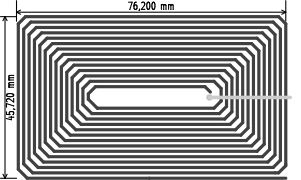
\includegraphics[width=0.6\textwidth]{placa_tag-brd}
	\caption{Antena del transponder fabricada sobre una placa de 
	circuito impreso. Su tamaño es el de una tarjeta ID--1 y su 
	inductancia \SI{8}{\micro\henry}.}
	\label{fig:DisenioAntena}
\end{figure}

% En la tabla \ref{tab:ParametrosAntena} se muestran, a modo de ejemplo, 
% los valores obtenidos luego de realizada la extracción de parámetros 
% del arreglo de antenas del la figura \ref{fig:ArregloDeAntenas} 
% utilizando como DUT el diseño de la figura 
% \ref{fig:DisenioAntena}.
% 
% \begin{table}
	% \centering
	% \begin{tabu}{lcl|lcl}
		% \toprule
		% Parámetro & Valor & Unidad & Parámetro & Valor & Unidad \\  
		% \midrule
		% \(L_{PICC}\)     & \SI{8.11}{}      & \si{\micro\henry} & \(k_{PICC,PCD}\) & \SI{0.062}{}     & -- \\
		% \(R_{PICC}\)     & \SI{1.51}{}      & \si{\ohm}         & \(k_{PICC,LA}\)  & \SI{0.198}{}     & -- \\
		% \(L_{PCD}\)      & \SI{0.47}{}      & \si{\micro\henry} & \(k_{PICC,LB}\)  & \SI{-0.019}{}    & -- \\
		% \(R_{PCD}\)      & \SI{0.167}{}     & \si{\ohm}         & \(k_{PCD,LA}\)   & \SI{0.092}{}     & -- \\
		% \(L_{A}\)        & \SI{0.368}{}     & \si{\micro\henry} & \(k_{PCD,LB}\)   & \SI{-0.092}{}    & -- \\
		% \(R_{A}\)        & \SI{0.388}{}     & \si{\ohm}         & \(k_{LA,LB}\)    & \SI{-0.026}{}    & -- \\
		% \(L_{B}\)        & \SI{0.368}{}     & \si{\micro\henry} &  \\
		% \(R_{B}\)        & \SI{0.388}{}     & \si{\ohm}         &  \\
		% \bottomrule
	% \end{tabu}
	% \caption{Parámetros extraídos mediante \emph{FastHenry} de la 
	% estructura de antenas de la figura \ref{fig:ArregloDeAntenas}.}
	% \label{tab:ParametrosAntena}
% \end{table}


% Diseño digital. Introducción, explicación del protocolo, arquitectura del 
% chip, microarquitectura de cada bloque, simulación, biblioteca estándar 
% utilizada, síntesis y place and route.
% Diseño digital. Introducción, explicación del protocolo (ya está en la 
% intro), arquitectura del chip, microarquitectura de cada bloque, 
% simulación, biblioteca estándar utilizada, síntesis y place and route. 
% Funciones desarrolladas para simular el diseño.
\chapter{Diseño digital}

El chip cuenta con un bloque digital que realiza un procesamiento 
mínimo de los datos recibidos para presentarlos en forma cruda 
---decodificados y desencapsulados--- en la interfaz digital de 
salida, donde serán utilizados por otros sistemas. Por otro lado 
también realiza el encapsulamiento y codificación de los datos a enviar 
a través del canal de RF,  generando para ello la señal de mando del 
bloque <<Modulador>>. Todo el procesamiento, desde las entradas 
hasta las salidas del bloque digital, se realiza utilizando lógica 
CMOS estática y es sincrónico con la señal portadora de 
\SI{13.56}{\mega\hertz} recibida en la antena. Sin embargo, dado 
que existen pausas en la portadora, el bloque digital también cuenta 
con un pequeño módulo asincrónico que ayuda a decodificar los datos 
recibidos.

El sistema digital fue diseñado utilizando el lenguaje descriptor de 
hardware \emph{Verilog} \cite{Verilog}, con el que se escribieron y 
probaron cada uno de los bloques por separado y luego todos en 
conjunto. La simulación del funcionamiento se realizó utilizando el 
software compilador/sintetizador \emph{Icarus Verilog} \cite{IVerilog} 
junto con \emph{GTKwave} \cite{GTKWave} para visualizar 
los resultados. La implementación del sistema digital fue realizada 
utilizando las herramientas de \emph{Synopsys Inc.} para síntesis (
\emph{Desing Compiler} \cite{SynopsysDC}) y place\&route (\emph{IC 
compiler} \cite{SynopsysICCompiler}), junto con la biblioteca de 
compuertas digitales de la Oklahoma State University (OSU) 
\cite{OSUstandardCells}. 

Para la verificación del funcionamiento a nivel lógico de cada uno 
de los bloques se desarrolló una estructura de pruebas que permitió enviar todas las combinaciones posibles de 
un byte de datos y comprobar su correcta recepción y transmisión. La 
estructura de pruebas consistió en varios \emph{tasks} de Verilog 
parametrizados de forma tal de poder indicar los datos a enviar.

En este capítulo se describirá la arquitectura del sistema digital y su 
funcionamiento. Se analizarán los módulos que conforman el bloque 
digital, su interconexión y se detallará el funcionamiento de cada uno 
de los ellos junto con las simulaciones realizadas. Por último se 
darán detalles acerca de la implementación con las herramientas de 
\emph{Synopsys}.


\section{Arquitectura}

\begin{figure}
	\centering
	\includegraphics[width=\textwidth]{DigitalBlockDiagram}
	\caption{Diagrama en bloques del sistema digital.}
	\label{fig:DigitalBlockDiagram}
\end{figure}

En la figura \ref{fig:DigitalBlockDiagram} se muestra un diagrama en 
bloques del sistema digital. El mismo puede dividirse en dos grandes 
partes que funcionan de forma independiente. Por un lado se 
tienen los módulos que conforman el bloque receptor de datos, 
compuesto por \lstinline{Bit Decoder} y \lstinline{Frame Receiver}, 
donde el primero identifica el comienzo de una trama y decodifica 
los bits recibidos, mientras que el segundo toma los bits 
decodificados y realiza la comprobación de las tramas, esto es, 
comprueba los bits de <<Inicio>>, <<Fin>> y <<Paridad>>. La carga 
útil dentro del frame es transmitida en serie a través de la salida 
\lstinline{rx_bit}, con \lstinline{rx_new_bit} señalizando el 
momento en que el dato es válido.

La recepción de datos se realiza a través de la entrada 
\lstinline{pause}, que es la señal de salida del detector de envolvente
y que se muestrea a una velocidad adecuada como para identificar cada 
bit. 

Por otro lado se tiene el bloque transmisor de datos, formado por 
\lstinline{Tx Buffer}, \lstinline{Frame Sender},
\lstinline{Frame Delay Counter} y \lstinline{Bit Encoder}. Los datos a 
transmitir a través de la interfaz de RF se ingresan en serie al 
buffer \lstinline{Tx Buffer} utilizando las entradas \lstinline{tx_bit}
y \lstinline{tx_new_bit}. El bloque transmisor permite ingresar de uno a 
ocho bits, que serán transmitidos encapsulados en una trama estándar 
luego de cumplido el tiempo de demora FDT. El módulo 
\lstinline{Frame Sender} es el encargado de agregar los bits de 
<<Inicio>>, <<Paridad>> y <<Fin>> correspondientes a la trama e 
iniciar la transmisión cuando recibe la señal del módulo 
\lstinline{Frame Delay Counter}. Los bits a transmitir son codificados 
en formato \emph{Manchester} por el módulo \lstinline{Bit Encoder} 
cuya función es también realizar la modulación OOK (ASK 100\%) con la 
señal sub-portadora de frecuencia \(\sfrac{f_{c}}{16}\). La salida 
\lstinline{coded_out} es la señal codificada y modulada que se conecta 
directamente al circuito modulador de carga.

La transmisión a través de la interfaz de RF debe comenzar luego de
transcurrida una cantidad exacta de ciclos de la señal portadora, 
comenzando a contar a partir de la recepción del símbolo de <<Fin>> 
de trama, según fue definido por el estándar y se vio en la figura 
\ref{fig:EsquemaFDT_PCD_PICC}. El módulo \lstinline{Frame Delay Counter}
se encarga de contar la cantidad de ciclos transcurridos a partir de que
se activa la señal \lstinline{rx_eof}, la cual señaliza el fin de trama 
(\emph{end of frame}), y al cumplirse el tiempo FDT activa la señal 
\lstinline{fdt} que habilita al bloque \lstinline{Frame Sender} a 
iniciar la transmisión. 
	
La señal portadora fue utilizada como reloj para el sistema digital, 
lo que tiene la ventaja de evitar el uso de un generador de reloj 
interno a la vez que sincroniza el transponder con el lector. Sin 
embargo, también tiene la desventaja de que la señal se interrumpe 
debido al esquema de codificación y modulación definido por el 
estándar (sección \ref{sec:ISO14443_2}). Entonces surge el 
inconveniente de que la señal \lstinline{pause} debe ser muestreada 
para decodificar los bits justo en el instante en que no hay reloj. 
Para superar este inconveniente se diseñó un pequeño circuito 
asincrónico que forma parte del módulo \lstinline{Bit Decoder} y 
cuya función es retener el estado de la señal \lstinline{pause} 
hasta que retorne el reloj y pueda ser muestreada.


\section{Recepción de datos}

La recepción de datos requiere de tres pasos: primero, con el detector 
de envolvente analógico se demodula la señal recibida para quitar la 
portadora y obtener la señal \lstinline{pause}, que es una 
representación digital de la envolvente. Luego se identifican los bits 
realizando un muestreo de \lstinline{pause} y finalmente se procesan 
los bits de control de la trama y se presenta la carga útil en la 
salida. 

En la figura \ref{fig:DecodedReception} se observa un ejemplo del 
proceso de recepción. Allí se observa como \lstinline{pause} 
cambia a estado `0' cada vez que ocurre una pausa en la entrada de 
RF y vuelve al estado lógico `1' cuando retorna la señal. La forma 
de \lstinline{pause} es similar a la de las secuencias X, Y y Z 
definidas por el estándar (figura \ref {fig:SecuenciasPCD_PICC}). 
Entonces basta con identificar cada una de esas secuencias y 
traducirlas a bits para obtener la información decodificada. Esta 
decodificación es la que se realiza el módulo \lstinline{Bit Decoder}
mediante el muestreo de la señal \lstinline{pause}.

\begin{figure}
	\centering
	\includegraphics{DecodedReception}
	\caption{Esquema del proceso de decodificación de los bits y 
	procesamiento de la trama recibida.}
	\label{fig:DecodedReception}
\end{figure}

Según la norma, la duración de cada bit es de 128 ciclos de 
portadora, mientras que la duración de las pausas es de 32 ciclos. 
Tomando cuatro muestras por bit centradas dentro del intervalo, es 
decir, en los ciclos 16, 48, 80 y 112, es posible identificar las 
tres secuencias unívocamente. La secuencia X representa los `1' 
lógicos e Y y Z representan los `0' lógicos.

Una vez decodificados los bits una máquina de estados se encarga de desencapsular la 
información contenida en la trama analizando para ello cada bit 
recibido. Todas las tramas ---ya sean cortas, estándar o anti-colisión 
(figura \ref{fig:TramasISO14443_3})--- comienzan con un bit de 
<<Inicio>> de comunicación, que se representa mediante un `0' y 
utilizando una secuencia Z. Esta secuencia tiene la característica de 
que la pausa se encuentra al inicio del tiempo del bit y por lo tanto 
al inicio de la comunicación. Entonces es posible utilizar esta primer 
pausa para sincronizar el traspaso de bits entre el lector y el 
transponder.

A continuación se reciben como máximo ocho bits de datos antes de 
recibir el bit de paridad. La trama puede finalizar antes con la 
recepción de un símbolo de <<Fin>> de comunicación (E: End) y en ese 
caso se tratará de una trama anticolisión, o de una trama corta si la 
cantidad de bits recibidos fue siete y son los primeros y únicos 
bits recibidos \footnote{Esta condición es debido a que podría darse 
el caso de que en una trama anti-colisión se divida un byte en el 
séptimo bit y que esos siete bits recibidos al final de la trama
sean equivalente a algún comando válido (REQA, WUPA, etc).}.

Una vez recibidos los ocho bits y comprobado el bit de paridad se 
señaliza el estado a través de las salidas \lstinline{rx_new_byte} y 
\lstinline{rx_par_error}. Si el bit de paridad fue correcto se procede 
a recibir otro byte a continuación, a menos que los dos bits 
siguientes sean el símbolo de <<Fin>>, en cuyo caso se activa la 
salida \lstinline{rx_eof} y el dispositivo entra en estado de reposo a 
la espera de un nuevo bit de <<Inicio>>.


\subsection{Módulo \lstinline{Bit Decoder}}

En la figura \ref{fig:BitDecoderBlockDiagram} se muestra un diagrama 
en bloques del módulo \lstinline{Bit Decoder}. El mismo está 
compuesto por un registro de desplazamiento de 4 bits en donde se toman
las muestras de la señal \lstinline{pause}, un contador que realiza el 
muestreo, otro que cuenta la cantidad de muestras tomadas, un 
multiplexor y una pequeña máquina de estados.

\begin{figure}
	\centering
	\includegraphics{BitDecoderBlockDiagram}
	\caption{Diagrama en bloques de <<Bit Decoder>>.}
	\label{fig:BitDecoderBlockDiagram}
\end{figure}

El módulo comienza en el estado de reposo \lstinline{IDLE} en el que 
espera a recibir la primer pausa. En este estado los contadores se 
mantienen en cero y no se toman muestras. Cuando se detecta que la señal 
\lstinline{pause} es igual a `0' ---esto es al final de la pausa, que 
es cuando retorna la señal de reloj--- se toma la primera muestra y el 
circuito pasa al estado \lstinline{IN_FRAME}.

En el estado \lstinline{IN_FRAME} se desplazan los bits del registro 
de desplazamiento cada 32 pulsos de reloj, entrando las nuevas 
muestras por el bit menos significativo. El contenido del registro de 
desplazamiento direcciona el multiplexor de forma tal de elegir 
\lstinline{data} y \lstinline{seq_z} en base a la secuencia recibida. 
Cuando el segundo contador cuenta cuatro muestras, se activa la señal 
\lstinline{new_bit} y se habilita el registro de salida.

El módulo \lstinline{Bit Decoder} no reconoce el fin de las tramas, 
ya que no es su función interpretar los datos recibidos, y por lo 
tanto queda en el estado \lstinline{IN_FRAME}, convirtiendo 
secuencias en bits, hasta que recibe la señal de fin de trama del 
módulo \lstinline{Frame Receiver}.

Por otro lado, existe el problema de que durante las pausas no se puede 
realizar ningún procesamiento, ya que el sistema digital se 
encuentra congelado en algún estado a falta de señal de reloj. Para 
superar este inconveniente, la detección de las pausas se realiza con 
la ayuda del circuito de la figura \ref{fig:PauseLatch}. Se trata de 
un circuito asincrónico que utiliza el flanco descendente de la señal 
\lstinline{env}, que es la envolvente de la portadora, para retener las
pausas y de esta forma generar la señal \lstinline{pause}. 

El circuito comienza con la salida \lstinline{pause} en `1'. Al 
producirse el primer flanco descendente en \lstinline{env} se 
dispara el flip-flop, la señal \lstinline{pause} pasa a `0' y queda 
retenida durante todo el tiempo en que no se tiene señal de reloj. En el 
primer flanco ascendente del reloj, la señal \lstinline{pause} es 
muestreada y luego se activa la señal \lstinline{release_pause}, que
libera la pausa forzando el estado del flip-flop a `1'. De esta forma 
es posible retener la pausas en la envolvente hasta que son 
interpretadas por el sistema digital.

\begin{figure}
	\centering
	\includegraphics{PauseLatch}
	\caption{Circuito asincrónico de retención de pausas.}
	\label{fig:PauseLatch}
\end{figure}


\subsection{Módulo \lstinline{Frame Receiver}}

El módulo \lstinline{Frame Receiver} se encarga de interpretar los 
bits de la trama y dejar la información útil disponible a la salida. 
Para ello recibe los bits de salida del módulo \lstinline{Bit Decoder}
que corresponden a las secuencias decodificadas, junto con las señales
que informan del estado, como son \lstinline{new_bit}, \lstinline{err},
etc.

En la figura \ref{fig:DiagramaFrameReceiver} se presenta un diagrama 
en bloques del módulo \lstinline{Frame Receiver}. Los bits 
decodificados por el módulo \lstinline{Bit Decoder} ingresan en dos 
registros de desplazamiento de dos bits cada uno. En el primero, 
\lstinline{data_buf}, se almacenan los bits decodificados y en 
\lstinline{seqz_buf} se almacenan unos lógicos sólo si los bits 
fueron representados mediante una secuencia Z.

\begin{figure}
	\centering
	\includegraphics[width=\textwidth]{FrameReceiver}
	\caption{Diagrama en bloques del módulo \lstinline{Frame Receiver}.}
	\label{fig:DiagramaFrameReceiver}
\end{figure}

El objetivo de estos pequeños buffers es poder detectar el símbolo de 
fin de comunicación que, como dice el estándar (sección 
\ref{sec:ISO14443_2}), está formado por un cero lógico seguido de una 
secuencia Y. En un principio se podría simplificar la definición 
diciendo que el fin de comunicación está representado por dos bits 
'0', ya que la secuencia Y también representa al cero lógico. Sin 
embargo se debe notar que la combinación de secuencias dada por el 
estándar no puede darse nunca durante la transmisión de datos, ya que
cualquier cero lógico tiene que estar representado por una secuencia 
Y o bien Z en caso de que el bit anterior haya sido un `0'. 
Entonces, un cero lógico seguido de una secuencia Y puede darse sólo 
en dos casos:

\begin{itemize}
	\item El último bit transmitido fue un `0', en cuyo caso el cero 
	lógico queda representado por una secuencia Z y entonces <<Fin>> = 
	ZY.
	
	\item El último bit transmitido fue un `1', y por lo tanto el cero 
	lógico es representado por una secuencia Y y entonces <<Fin>> = 
	YY.
\end{itemize}

En ambos casos la secuencia de bits representados es `00', sin 
embargo, de tratarse de dos ceros dentro de la trama, con información, 
las secuencias utilizadas serían ZZ en el primer caso, e YZ en el 
segundo. 

Teniendo en cuenta las diferencias en el orden de las secuencias Z en 
uno y otro caso se desarrolló el sistema de detección del símbolo 
<<Fin>>. El circuito combinacional de la figura 
\ref{fig:DiagramaFrameReceiver} activa la señal de \lstinline{stop},
que indica que fue encontrado el símbolo de fin de comunicación, 
sólo cuando el buffer de datos contiene la secuencia `00' y 
\lstinline{seqz_buf} contiene `10' o `00'.

De forma similar se detecta el bit de <<Inicio>> de comunicación, 
que está representado por una secuencia Z. La señal \lstinline{start} 
se activa cuando \lstinline{data_buf[0]=1b'0} y 
\lstinline{seqz_buf[0]=1b'1}.

La salida del buffer de datos está conectada directamente al buffer de 
salida \lstinline{byte_buf}, donde se almacena la carga útil de la 
trama. La lógica de control habilita de forma selectiva el 
buffer de salida de forma tal de descartar los bits de <<Inicio>>, 
<<Fin>> y <<Paridad>>, y almacenar allí solo los datos contenidos
en la trama. Los bits de \lstinline{byte_buf} se desplazan de MSB a LSB,
por lo tanto, en caso de recibir una trama corta que contiene sólo 
comandos de 7 bits (REQA, WUPA,\...), éstos quedarán almacenados en 
los bits más significativos de la salida, \lstinline{data_byte[7:1]}.

Cada nuevo bit que se almacena en el buffer de salida se señaliza con 
la salida \lstinline{new_bit}. Del mismo modo, cuando se completan los 
ocho bits de \lstinline{data_byte}, se activa la señal 
\lstinline{new_byte}; en caso de producirse un error de paridad se 
activa \lstinline{par_error}; y por último, al detectar el símbolo 
<<Fin>> se activa la señal \lstinline{eof}. Todas estas señales son 
pulsos de un ciclo de reloj de duración y además forman parte de la 
salida de datos del circuito integrado. 

La señal \lstinline{new_bit} es útil en el caso de recibir una trama 
anti-colisión, que puede estar dividida en cualquier bit. En este caso 
el sistema externo al chip puede recibir los bits de a uno, leyendo el 
dato de \lstinline{data_byte[7]} cada vez que \lstinline{new_bit} es 
igual a `1'; o puede recibir los datos de a bytes, y en el byte 
dividido contar la cantidad de bits con \lstinline{new_bit} y leer 
sólo los datos válidos de \lstinline{data_byte}.

En una trama estándar, luego de recibidos los ocho bits de datos se 
debe chequear el bit de paridad. El estándar dice que el bit de 
paridad debe ser tal que la cantidad de unos lógicos en la dupla 
\lstinline{[data,P]} debe ser impar. Para corroborar que esto se 
cumpla en las tramas recibidas, se implementó un circuito generador 
de paridad como el de la figura \ref{fig:ParityChequer}. Por cada 
bit \(b_{n}\) que es recibido, se realiza la operación \(P_{n+1} = 
b_{n} \oplus P_{n}\), donde \(P_{n}\) es el resultado de la 
operación anterior y su valor inicial es `0'. Observando la tabla de 
verdad, el resultado de esta operación es `1' si la cantidad de bits 
recibidos en estado `1' es impar. Por ejemplo, si \(P_{n}=0\) y se 
recibe un bit en `1', el resultado de la XOR es `1', indicando que 
la cantidad de unos recibidos hasta el momento es impar. Si se 
recibe otro `1', entonces \(1 \oplus 1 = 0\), lo que indica que se 
tiene una cantidad par de unos lógicos.

\begin{figure}
	\centering
	\includegraphics[]{ParityChequer}
	\caption{Circuito generador de bit del bit de paridad.}
	\label{fig:ParityChequer}
\end{figure}

Este procesamiento se realiza con los bits de datos recibidos, dejando 
afuera los bits de <<Inicio>> y <<Fin>>. Al recibir el bit de paridad 
se compara con el calculado hasta el momento por el circuito generador 
de paridad. Si ambos bits coinciden, los datos fueron recibidos 
correctamente y se sigue adelante con el procesamiento. Si los bits no 
coinciden se activa la señal \lstinline{par_error}, informando de esta 
manera al sistema externo que utiliza los datos.


\section{Transmisión de Datos}

Para transmitir datos hacia el lector, primero se carga el buffer de 
transmisión \lstinline{Tx buffer} de a un bit por vez utilizando las 
entradas \lstinline{tx bit} y \lstinline{tx new bit} de la figura 
\ref{fig:DigitalBlockDiagram}. El módulo \lstinline{Tx buffer} no es 
más que un registro de desplazamiento con entrada serie y salida 
paralelo, que se habilita con la señal \lstinline{tx new bit}, más 
un contador de 3 bits que cuenta los N bits que ingresan al registro. 
Por cada flanco ascendente de reloj, si la señal \lstinline{tx new bit} 
está en alto se desplaza un bit y se incrementa la cuenta.

Los datos y la cuenta del buffer ingresan al módulo 
\lstinline{Frame Sender} y este se encarga de encapsular la información 
en la trama, que luego es enviada a través de la interfaz de RF. Cuando 
se recibe la señal \lstinline{tx transmit}, que indica que se debe 
transmitir el contenido del buffer, los datos y la cuenta son pasados a 
registros internos de \lstinline{Frame Sender} y se reinicia el 
contador, dejando el buffer listo para una nueva carga. Esto permite que 
el dispositivo externo que controla al circuito integrado pueda 
cargar el buffer con el siguiente bloque de datos aunque exista una 
transmisión en curso. De esta forma se agiliza la transmisión sin la 
utilización de un buffer de mayor tamaño.

La transmisión de datos se inicia cuando que se cumple el tiempo de 
demora entre tramas FDT (\emph{Frame Delay Time}). El FDT es 
controlado por el módulo \lstinline{Frame Delay Counter}, que cuenta 
la cantidad de ciclos de reloj transcurridos desde que se recibe el 
símbolo de <<Fin>> de comunicación, señalizado por \lstinline{rx eof}. 

Los bits a enviar son codificados en código \emph{Manchester} por el 
módulo \lstinline{Bit Coder}, quién también agrega la subportadora y 
maneja las llaves que actúan en la modulación de carga (Estas llaves 
se verán más adelante en la sección \ref{sec:Modulador}). El módulo 
\lstinline{Bit Coder} se encarga además de controlar la duración 
de cada bit, que es de 128 ciclos de portadora, y una vez finalizada la 
transmisión de un bit informa a \lstinline{Frame Sender} que se 
encuentra disponible para enviar el siguiente bit. La salida 
\lstinline{coded_out} se conecta directamente al bloque Modulador y la 
información codificada es transmitida hacia el lector.

Las tramas enviadas comienzan con el bit de <<Inicio>> de 
comunicación, luego se transmiten los N bits que fueron cargados en 
el buffer y por último el bit de paridad. Si bien las tramas estándar 
(figura \ref{fig:TramaEstandarISO14443_3}) contienen bloques de 8 bits 
más el bit de paridad, es imprescindible contar con la posibilidad de 
enviar bloques de menor tamaño para poder contestar a las tramas 
anti-colisión (figura \ref{fig:TramaAnticolISO14443_3}) de las que en 
principio no se sabe en que punto pueden ser divididas.

Un ciclo de reloj antes de que finalice la transmisión del bit de paridad,
\lstinline{Frame Sender} activa la señal \lstinline{tx ready} que 
informa al dispositivo controlador que el circuito está 
listo para recibir una nueva orden de transmisión. Si no se recibe la 
orden, la trama finaliza con el símbolo de <<Fin>> y 
\lstinline{Frame Sender} vuelve al estado de reposo. Si la orden es 
recibida en el instante en que termina de enviarse el último bit, la 
transmisión previa continúa y no se envía un nuevo bit de <<Inicio>> 
sino que se continúa con la trama anterior. 

Esto es útil para las tramas estándar o anti-colisión, que contienen 
más de un byte, donde los bits deben transmitirse de forma continua 
para no dividir la trama, lo que podría ocasionar errores en la 
comunicación. El mecanismo de transmisión implementado maneja de 
forma autónoma el inicio y fin de las tramas, decidiendo 
automáticamente si debe agregar o no el bit de <<Inicio>> de 
comunicación basado en el instante en que recibe la señal 
\lstinline{tx transmit}.


\subsection{Módulo \lstinline{Frame Sender}}

\begin{figure}
	\centering
	\includegraphics[]{FrameSender}
	\caption{Diagrama del módulo \lstinline{Frame Sender}.}
	\label{fig:FrameSenderDiagBloques}
\end{figure}

En la figura \ref{fig:FrameSenderDiagBloques} se muestra un diagrama 
del módulo \lstinline{Frame Sender}. La maquina de estados controla un 
par de registros ---donde se almacenan los datos a transmitir y la 
cantidad de bits---, un multiplexor y un generador de paridad como el 
de la figura \ref{fig:ParityChequer}.

Al recibir la señal \lstinline{transmit}, la máquina de estados 
carga los buffers de entrada con los datos del módulo 
\lstinline{Tx Buffer} e inicializa un contador interno que lleva la 
cuenta de la cantidad de bits enviados hasta el momento. Luego espera 
a recibir la señal \lstinline{fdt}, que le indica que el tiempo FDT se
ha cumplido, y que puede iniciar la transmisión. En el diagrama de 
tiempos de la figura \ref{fig:FrameSenderDiagTiempos} se muestra un 
ejemplo de transmisión. Allí pueden seguirse los pasos realizados por 
\lstinline{Frame Sender} junto con el diagrama de estados de la figura 
\ref{fig:FrameSenderDiagEstados}.

\begin{figure}
	\centering
	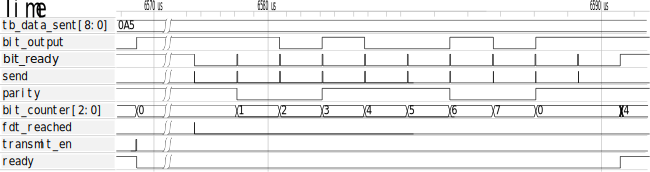
\includegraphics[width=\linewidth]{tb_FrameSender.pdf}
	\caption{Diagrama de tiempos del módulo \lstinline{Frame Sender}.}
	\label{fig:FrameSenderDiagTiempos}
\end{figure}

\begin{figure}
	\centering
	\includegraphics[]{DiagramaEstadosFrameSender}
	\caption{Diagrama de estados del módulo \lstinline{Frame Sender}.}
	\label{fig:FrameSenderDiagEstados}
\end{figure}

Una vez recibida la señal \lstinline{fdt} comienza la transmisión 
direccionando el primer bit con el multiplexor, que siempre es el 
bit de <<Inicio>> de comunicación, y enviando un 
pulso a través de \lstinline{send} al módulo \lstinline{Bit Coder}. 
Este módulo se encarga de codificar el bit y de generar la señal de 
manejo del modulador de carga. 

Cuando \lstinline{Bit Coder} finaliza la transmisión, activa 
la señal \lstinline{bit_ready}, informando que se encuentra disponible 
para enviar otro bit. Al recibir esta señal la máquina de estados 
direcciona el bit siguiente, \(d_{0}\), nuevamente envía un pulso a 
través de \lstinline{send}, y luego espera a que se active la señal 
\lstinline{bit_ready} antes de continuar. Cuando finaliza el envío de 
\(d_{0}\) se continua con \(d_{1}\), luego \(d_{2}\) y así 
sucesivamente.

Como la cantidad de bits en el registro de entrada puede ser menor a 
ocho, el proceso se repite hasta que la cantidad de bits enviados, o lo 
que es lo mismo, la dirección del multiplexor, sea igual a la cantidad 
de bits cargados en \lstinline{Tx Buffer}. Cuando esto se cumple se 
pasa automáticamente a la dirección del bit de paridad \(P\). En caso 
contrario,  
se continúa incrementando la dirección hasta enviar todos los bits y 
llegar a \(P\), lo que sucederá cada vez que se envíe una trama 
estándar con ocho bits de datos.

El bit de paridad se calcula del mismo modo que en el módulo 
\lstinline{Frame Receiver}, sólo que en este caso se utilizan para 
el cálculo los bits de salida del multiplexor. Al finalizar la 
transmisión del bit de <<Inicio>>, el bloque generador de paridad es 
reiniciado por la máquina de estados. Luego, a medida que los bits 
de datos son seleccionados, se hacen ingresar al generador hasta que 
finalmente, cuando se selecciona \(P\), se toma su salida y se envía 
en la posición del bit de paridad. De esta forma se cumple siempre el 
requerimiento del estándar de enviar los datos con paridad impar.

Por último, cuando \lstinline{Bit Coder} informa que finalizó
la transmisión del último bit, la máquina de estados activa la señal 
\lstinline{ready} que informa al circuito o dispositivo externo que finalizó la 
transmisión. Esto sucede en realidad un ciclo de reloj antes de que el 
último bit termine y permite que, en caso de recibir una nueva orden de 
transmisión durante el ciclo de reloj siguiente a la activación de 
\lstinline{ready}, se continúe la trama enviando un nuevo bloque de 
datos más paridad sin bit de <<Inicio>>. Cuando esto ocurre, se cargan
los registros de entrada con los datos de \lstinline{Tx Buffer}, se 
direcciona directamente el bit \(d_{0}\) y se repite el proceso de 
envío.

Si \lstinline{transmit} no se activa durante el ciclo de reloj 
siguiente al flanco ascendente de \lstinline{ready}, la trama se 
da por terminada y la máquina de estados vuelve al estado de reposo.


\subsection{Módulo \lstinline{Bit Coder}}

\begin{figure}
	\centering
	\includegraphics[]{BitCoder}
	\caption{Diagrama del módulo \lstinline{Bit Coder}.}
	\label{fig:BitCoderDiagBloques}
\end{figure}

El módulo \lstinline{Bit Coder} se encarga de codificar los bits que 
deben ser enviados a través de la interfaz de RF como especifica el 
estándar (ver tabla \ref{tab:CodificacionPICC_PCD}) y generar la señal 
de comando del modulador de carga. 

En la figura \ref{fig:BitCoderDiagBloques} se muestra un diagrama de 
los componentes internos del módulo. Allí se observa que el mismo 
está compuesto por un bloque codificador \emph{Manchester}, un 
divisor de frecuencia y una compuerta AND. La salida \lstinline 
{coded_out} es la señal de comando de la llave que conecta la carga 
en el bloque modulador analógico. Cuando \lstinline{coded_out} es 
igual a `1' la llave se cierra y por lo tanto se dice que la 
portadora está \emph{cargada}. Por otro lado, cuando 
\lstinline {coded_out} es `0' la llave está abierta y no se carga a 
la señal de RF.

El Codificador Manchester se encarga de generar el código  
a partir de los bits de entrada. En el estado de reposo su salida se 
mantiene en `0' y por lo tanto la salida del módulo 
\lstinline{coded_out} también. Al recibir un pulso en la entrada 
\lstinline{send} produce en su salida el código Manchester 
correspondiente al estado de \lstinline{bit_in}. Cada bit codificado 
tiene la duración especificada por el estándar, es decir, 128 ciclos 
de reloj. Al finalizar con el código activa la señal 
\lstinline{ready} y vuelve al estado de reposo.

Por otro lado, el divisor de frecuencia divide la señal de reloj de 
\SI{13.56}{\mega\hertz} por 16 para generar la señal sub-portadora 
de \SI{848}{\kilo\hertz}. El estándar especifica que la modulación 
de carga al inicio de cada bit debe tener una fase definida, es por 
ello que se incluyó en el divisor de frecuencia la entrada 
\lstinline {init}. Según la norma, los bits deben comenzar con el 
estado \emph{cargado} de la señal de RF y entonces la entrada 
\lstinline{init} sirve para forzar el estado de la salida del divisor 
de frecuencia a `1' cada vez que comienza la transmisión de un bit.

Finalmente, la operación AND de los bits codificados en código 
Manchester con la señal sub-portadora da como resultado las secuencias 
definidas en la tabla \ref{tab:CodificacionPICC_PCD}. 

Un detalle importante es que \lstinline{Bit Coder} informa que finalizó
la transmisión de un bit un ciclo antes de que la transmisión 
realmente termine. Esto es debido a que se debe permitir continuar 
la con la trama con un nuevo pulso en \lstinline{send} sin 
interrumpirla ni dejar espacios entre bits. 


\section{Verificación funcional}

La verificación del funcionamiento fue realizada módulo por módulo y 
luego del sistema completo utilizando para ello el conexionado que 
realiza el eco de un byte.

Los \emph{testbenchs}\footnote{Bancos de prueba codificados en lenguaje
\emph{Verilog}} desarrollados permitieron generar las señales de 
entrada del sistema digital y enviar datos con tan solo llamar a un 
\emph{task} de \emph{Verilog}, pasando como argumento el valor a 
enviar. 

Los \emph{tasks} de más bajo nivel generan el patrón de envolvente de 
la portadora correspondiente a las secuencias X, Y o Z. El patrón de 
envolvente se utiliza para generar la señal \lstinline{pause} y a la 
vez, a través de una operación AND lógica, se detiene el reloj del 
sistema. De esta forma se simula lo que sucede realmente al arribar 
una pausa en la portadora. También se codificaron \emph{tasks} para 
generar las secuencias de <<Inicio>> y <<Fin>> de comunicación y luego 
se escribió un \emph{task} de más alto nivel que utiliza a los 
anteriores para enviar cualquier bytes de datos pasado como parámetro. 

Con los \emph{tasks} desarrollados se pudieron enviar las tramas de 
entrada al sistema digital y verificar la respuesta del mismo. Para 
probar el sistema de recepción de información se desarrollo un 
\emph{testbench} que envía los bytes de 8'h00 a 8'hFF, de a uno por 
vez y armando la trama completa, es decir, <<Inicio>> + datos + 
<<Paridad>> + <<Fin>> y comprueba automáticamente que a la salida de 
\lstinline{Frame Receiver}, en el registro \lstinline{byte_buf}, quede 
almacenado el valor correcto cuando se genera el pulso en 
\lstinline{new_byte}. Las pruebas realizadas de esta forma permitieron 
depurar el diseño hasta obtener un sistema de recepción de 
información libre de errores.

Por otro lado, para el sistema de transmisión de información el 
\emph{testbench} desarrollado constó del envío de algunos bytes 
típicos, que fueron cargados manualmente en el buffer de transmisión, 
y la verificación se hizo mediante el análisis del diagrama de 
tiempos del sistema. En este caso no se desarrolló un test 
automatizado debido a la dificultad de leer y verificar la señal 
\lstinline{coded_out}, que está formada por el código 
\emph{Manchester} modulado con la sub-portadora, mediante código en 
\emph{Verilog}. Sin embargo, también se hizo la prueba exhaustiva 
de enviar los 256 bytes de datos posibles utilizando para ello el 
conexionado de la interfaz de recepción con la de transmisión, como 
se verá a continuación.

\subsection{Eco de un byte}

En la figura \ref{fig:DigitalBlockDiagram} se muestra en líneas 
punteadas como puede conectarse directamente la salida del bloque
receptor con la entrada del bloque transmisor para obtener un \emph{tag} 
autónomo que realiza el eco de un byte, es decir, devuelve al lector 
el byte de datos recibido. Al conectar el dispositivo de esta forma, 
los bits recibidos en \lstinline{rx_bit} ingresan directamente al 
buffer de transmisión. Al finalizar la trama y detectarse el símbolo 
de <<Fin>> se activa la señal \lstinline{rx_eof}, que a su vez sirve 
de señal de inicio de transmisión a través de \lstinline{tx_transmit}.

El diseño puede retransmitir sólo un byte de datos, ya que el buffer de 
transmisión tiene el tamaño de un byte y se sobreescribe si se recibe una 
cantidad de datos mayor.

En la figura \ref{fig:SimulacionDigital} se muestra una simulación a 
nivel lógico del bloque digital con la conexión que produce el eco. 
Allí se observa como el dispositivo recibe el byte de datos, 8h'53 
en este caso, a la vez que lo carga en el buffer e inicia la 
transmisión luego de cumplido el FDT. Las señales 
\lstinline {tb_rx_bit} y \lstinline{tx_bit} son los bits recibidos y 
a cargar en el buffer, mientras que \lstinline{tb_rx_new_bit} indica 
que el bit es un nuevo bit válido para la lectura y 
\lstinline {tx_new_bit} es la señal que habilita la carga del buffer 
de transmisión en el siguiente flanco ascendente de reloj.

Se debe notar que los bits se reciben en orden \emph{LSB First}, es 
decir, se recibe primero el bit menos significativo. El 
buffer de transmisión fue diseñado para ser cargado también en ese 
orden, lo que evita el uso de componentes externos.

\begin{figure}
	\centering
	\includegraphics[width=\textwidth]{tb_top_phy_layer}
	\caption{Simulación del bloque digital cuando el dispositivo es 
	utilizado en modo \emph{eco}.}
	\label{fig:SimulacionDigital}
\end{figure}

En el \emph{testbench} desarrollado para verificar la funcionalidad 
del modo \emph{eco} se enviaron los 256 bytes de datos posibles al 
sistema digital y todos fueron reenviados a través de 
\lstinline{coded_out} correctamente.

\section{Implementación: Síntesis y \emph{Place\&Route}}

La descripción del hardware en lenguaje \emph{Verilog} fue 
sintetizada utilizando el software \emph{Synopsys Design Compiler} 
\cite{SynopsysDC} junto con la biblioteca de celdas digitales de la 
\emph{Oklahoma State University} (OSU), celdas que fueron diseñadas 
para el proceso de fabricación C5N de \emph{ON Semiconductor}. 

La biblioteca incluye compuertas lógicas NAND, NOR, XOR, inversores, 
AOI, OAI, etc., junto con buffers especiales para el árbol de 
distribución de reloj, multiplexores y flip-flops tipo D disparados 
por flanco \hyphenation{as-cen-den-te/des-cen-den-te}ascendente/descendente. 
Todas las celdas están caracterizadas en cuanto a tiempos de 
propagación para todos los caminos posibles entre entradas y 
salidas, cuentan con características dinámicas de las salidas, como 
son los tiempos de crecimiento/decrecimiento y consumo de potencia 
dinámica según la capacidad de carga.

La herramienta de síntesis utiliza la caracterización de las 
compuertas junto con restricciones impuestas al diseño para 
optimizar los tiempos de retardo y el área ocupada por el circuito. 
La frecuencia de operación es la primer restricción de todo circuito 
sincrónico y en este caso es de \SI{13.56}{\mega\hertz}. Sin embargo, 
para contar con un margen de seguridad en caso de que el retardo de 
las compuertas fuese mayor al esperado por variaciones del proceso, se impuso como restricción una 
frecuencia de operación de \SI{15}{\mega\hertz}. 

Por otro lado, para reducir el consumo de potencia se activó la 
opción de la herramienta de síntesis que hace uso de la técnica 
\emph{clock gating}. Esta técnica agrega una pequeña lógica en la entrada 
de reloj de los flip-flops que permite activar o desactivar esa señal. 
Cuando un FF debe mantener el estado de su salida durante varios ciclos
de reloj, como por ejemplo los FF siguientes al primero de un contador 
binario, se desactiva la señal de reloj en su entrada para evitar el consumo de 
potencia dinámica debido a la transición del reloj de un estado a otro.

El trazado físico del diseño (\emph{Place\&Route}) se realizó con el 
software \emph{Synopsys IC Compiler} \cite{SynopsysICCompiler}. En 
este caso se le debe indicar al programa la forma o tamaño deseado. 
Como el área ocupada en general se desea que sea la mínima posible, 
se suele definir entonces la relación de aspecto alto/ancho del 
trazado deseado. También se le deben indicar las posiciones de las 
entradas y salidas del bloque, que luego serán conectadas con el resto 
del los circuitos. 

El programa ubica las compuertas optimizando las 
posiciones según el conexionado. Luego genera un árbol de reloj y 
finalmente realiza el conexionado de todas las compuertas. El 
\emph{layout} final del bloque digital puede verse en la figura 
\ref{fig:LayoutBloqueDigital}.

\begin{figure}
	\centering
	\includegraphics[width=\linewidth]{Layout_digital}
	\caption{\emph{Layout} final del bloque digital. Sus dimensiones 
	son de \SI{900}{\micro\meter} \(\times\) \SI{330}{\micro\meter}.}
	\label{fig:LayoutBloqueDigital}
\end{figure}

Las herramientas generan una serie de reportes del área ocupada, el 
tiempo de retardo del camino crítico y los registros en que se 
utilizó la técnica de \emph{clock gating}. En la tabla 
\ref{tab:AreaDigital} se presenta un resumen del área ocupada por cada 
uno de los módulos del diseño luego de la síntesis lógica y sin 
tener en cuenta el árbol de distribución de reloj ni el área 
necesaria para el conexionado de las compuertas. El módulo 
\lstinline{frame_sender} es el de mayor tamaño, mientras que los 
demás son de tamaños similares, salvo \lstinline{pause_latch} y 
\lstinline{rst_sync}\footnote{Este módulo es el circuito sincronizador 
de la señal de reset.}, que al contener un registro el primero y dos el 
segundo son de tamaño despreciable. 

\begin{table}
	\centering
	\begin{tabu}{lc}
		\toprule
		Módulo & Area \(\left[\si{\micro\meter\squared}\right]\) \\  
		\midrule
		\lstinline{bit_coder}              & 33669 \((15.1\%\)) \\
		\lstinline{bit_decoder}            & 37791 \((16.9\%\)) \\
		\lstinline{frame_delay_counter}    & 28656 \((12.8\%)\) \\
		\lstinline{frame_receiver}         & 36972 \((16.6\%)\) \\
		\lstinline{frame_sender}           & 57447 \((25.8\%)\) \\
		\lstinline{pause_latch}            & 1800  \((0.1\%)\) \\
		\lstinline{rst_sync}     & 3600  \((0.2\%)\) \\
		\lstinline{tx_buffer}              & 22563 \((10.1\%)\) \\
		\midrule
		Total 8 Módulos        &         222498\\
		\bottomrule
	\end{tabu}
	
	\caption{Área utilizada por cada uno de los módulos luego de la 
	síntesis.}
	
	\label{tab:AreaDigital}
\end{table}

En la tabla \ref{tab:ResumenClockGating} puede verse un resumen del 
reporte de la herramienta de síntesis luego de aplicar la técnica 
de \emph{clock gating}. De los 95 registros del diseño, a 70 
se les pudo aplicar esta técnica para reducir el consumo. El software 
también estima la potencia consumida por las compuertas trabajando a 
la frecuencia establecida. Luego de aplicar la técnica de \emph{clock 
gating} la potencia dinámica estimada por el sintetizador se redujo 
un 30\%, de \SI{3.43}{\milli\watt} a \SI{2.39}{\milli\watt}.

Sin embargo, el agregado de las celdas de \emph{clock gating}, cuyo 
esquemático puede verse en la figura \ref{fig:CeldaClockGating}, tiene 
el inconveniente de que disminuye el tiempo disponible para el arribo 
de la señal proveniente de la lógica. Esto es debido a que el latch 
del esquemático actúa cuando el reloj está en nivel bajo, mientras que 
los flip--flops del resto del diseño trabajan por flanco ascendente. 
Entonces, luego de un flanco ascendente de reloj, la entrada 
\lstinline{Gate} tiene sólo medio período para establecerse antes de 
que actúe el latch en el siguiente nivel bajo. Esto afectará el 
camino crítico como se verá a continuación.

\begin{figure}
	\centering
	\includegraphics[]{ClockGatingCell}
	\caption{Celda de \emph{clock gating} construida por el 
	sintetizador.}
	\label{fig:CeldaClockGating}
\end{figure}

\begin{table}
	\centering
	\begin{tabu}{lc}
		\toprule
		\multicolumn{2}{c}{Resumen de \emph{Clock Gating}} \\
		\midrule
		Cantidad total de registros                   &      95      \\
		Cantidad de celdas de \emph{clock gating}  & 13           \\
		Cantidad de registros con \emph{clock gating} & 70 \((73.68\%)\) \\
		Cantidad de registros sin \emph{clock gating} & 25 \((26.32\%)\) \\
		\bottomrule
	\end{tabu}
	
	\caption{Resultado arrojado por la herramienta de síntesis luego de
	aplicar la técnica de \emph{clock gating} al diseño.}
	
	\label{tab:ResumenClockGating}
\end{table}

Finalmente, utilizando las características de retardos y capacidad de 
entradas y salidas, la herramienta calcula el retardo de las señales 
entre registros para ver que se cumpla con la frecuencia de operación 
requerida. En caso de que el retardo sea mayor al período de reloj el 
software optimiza las dimensiones de las compuertas o agrega buffers, 
incrementando el área ocupada, para intentar cumplir con la frecuencia de 
operación indicada. El parámetro que se toma como referencia para 
saber si se cumple o no es el \emph{slack time}, que es el tiempo 
entre que arriba la señal de datos a la entrada de un registro hasta 
que arriba el flanco de reloj. Si el \emph{slack time} fuese negativo 
el circuito no podría funcionar. Luego de la síntesis se genera un 
informe con los tiempos de retardo de cada uno de los caminos posibles 
entre registros. Al camino con menor \emph{slack time} se lo denomina 
\emph{camino crítico} y es el primero que debe optimizarse. 

En la tabla \ref{tab:DigitalCaminoCritico} se muestra el reporte del 
camino crítico para el diseño. El camino parte de la entrada 
\lstinline{tx_transmit} y termina en un FF del módulo 
\lstinline{Frame Sender}. Una de las restricciones impuestas para 
forzar un peor caso es que todas las entradas tengan un retardo de 
\SI{10}{\nano\second} y por este motivo es que en la tabla el 
\emph{input delay} comienza con ese valor. El software suma el retardo 
de las compuertas hasta llegar al registro al final del camino. El 
\emph{data arrival time} es el resultado de la suma, que se compara con el
\emph{data required time} generalmente dado por la frecuencia de trabajo. 
Debido a la utilización de las celdas de \emph{clock gating}, que como 
se dijo reducen el tiempo disponible para el establecimiento de la 
lógica, el \emph{data required time} fue de la mitad del período de 
reloj. Finalmente, el \emph{slack} calculado para el camino crítico fue de 
\SI{22.18}{\nano\second} y no fue necesario intervenir en la síntesis.

\begin{table}
	\centering
	\begin{tabu}{lc}
		\toprule
		Punto            & Retardo \(\left[\si{\nano\second}\right]\) \\
		\midrule
		Input external delay        &   10.00 \\
		frsen/U13/Y (INVX2)         &   10.07 \\
		frsen/U65/Y (NOR2X1)        &   10.28 \\
		frsen/U74/Y (NAND2X1)       &   10.70 \\
		frsen/U81/Y (OAI22X1)       &   10.82 \\
		Data arrival time           &   10.82 \\
		\addlinespace
		Clock clk' (rise edge)      &   33.00 \\
		Clock network delay (ideal) &   33.00 \\
		\midrule
		Data required time          &   33.00 \\
		Data arrival time           &  -10.82 \\
		\midrule
		Slack (MET)                 &   22.18 \\
		\bottomrule
	\end{tabu}
	
	\caption{Retardos del camino crítico: Desde \lstinline{tx_transmit} 
	hasta \lstinline{frsen/clk_gate_bits_to_send_ret_reg/latch}.} 
	%\footnote{\lstinline{frsen} es \lstinline{frame_sender}}.}
	
	\label{tab:DigitalCaminoCritico}
\end{table}

Luego, mediante una simulación a nivel de transistor se obtuvo la 
corriente promedio de consumo del bloque digital, que fue de 
\SI{325}{\micro\ampere} a \SI{3}{\volt}, lo que da una potencia 
ligeramente menor a la estimada por el sintetizador.


% Diseño Analógico. Introducción, características de las señales según el 
% estándar, arquitectura del circuito, acondicionamiento de la energía 
% (rectificadores, regulador, Iref), detector de envolvente, extracción de 
% reloj y POR. Simulaciones, mediciones.
% Diseño Analógico. Introducción, características de las señales 
% según el estándar, arquitectura del circuito, acondicionamiento de 
% la energía (rectificadores, regulador, Iref), detector de 
% envolvente, extracción de reloj y POR. Simulaciones, mediciones. 
\chapter{Diseño Analógico}

En este capítulo se realizará un recorrido por los bloques 
analógicos del circuito integrado. El diseño analógico comprende 
cuatro sistemas que hacen de soporte al bloque digital y que se 
verán a continuación. El primero de ellos es el sistema de captura y 
acondicionamiento de la energía, que debe tomar la energía recibida 
a través de la señal portadora, almacenarla y acondicionarla para 
ser usada por los demás bloques del circuito integrado. En segundo 
lugar se verá el sistema de transmisión y recepción de datos, que 
por un lado se encarga de demodular la señal enviada por el lector y 
adaptarla a los niveles lógicos del bloque digital; y por otro 
realiza la modulación de carga sobre la señal portadora para 
transmitir hacia el lector. Luego se verá el sistema de captura y 
reconstrucción de la señal de reloj a partir de la portadora de 
\SI{13.56}{\mega\hertz} y para finalizar se analizará el 
\emph{power-on reset}, que inicializa la lógica digital a través de la 
señal \lstinline{reset} cuando la tensión de alimentación alcanza el 
nivel de operación.


\section{Acondicionamiento y uso de la energía}

Como se vio en la sección \ref{sec:TransmisionDeLaEnergia} la amplitud 
de la tensión en la antena varía con la distancia entre el lector y 
el transponder durante la operación normal del dispositivo. Por este 
motivo es que se implementó el bloque <<Regulador/Limitador de 
tensión>>, que tiene como objetivo mantener la tensión a la entrada 
de la antena dentro del nivel de funcionamiento a pesar de las 
variaciones de la distancia al lector o, lo que es lo mismo, las 
variaciones en el coeficiente de acoplamiento. Para lograrlo la idea 
es cargar a la antena con una carga interna dentro del transponder 
de forma tal de cancelar las variaciones de amplitud 
debidas a los cambios en el coeficiente de acoplamiento. 

Por otra parte se debe tomar la tensión alterna generada en la antena, 
rectificarla y filtrarla para ser usada como tensión de alimentación 
dentro del chip. Esto se hace con el bloque <<Rectificador + Filtro>> 
de la figura \ref{fig:DiagramaEnBloquesCI}. Entonces se tiene por un 
lado el regulador de tensión que actúa de carga variable, y por otro la
toma de energía a través del bloque <<Rectificador + Filtro>>, ambos 
conectados a la entrada de la antena.

\subsection{Regulador/Limitador de tensión}

Se trata de un regulador de tensión de tipo paralelo y la idea es 
ajustar una carga variable de forma tal de regular la tensión 
inducida en la antena, manteniéndola por debajo del límite de 
tensión máxima permitida por el proceso de fabricación CMOS.

En la figura \ref{fig:ReguladorCircuito} se muestra el regulador 
propuesto. La tensión alterna de la antena en los nodos \(rf_{1}\) y 
\(rf_{2}\) es convertida mediante el rectificador de onda completa a 
tensión continua en el nodo \(V_{reg}\). A la salida del 
rectificador se encuentra conectada la carga variable, que fue 
implementada con un transistor NMOS, y es controlada por la señal de 
error que produce el amplificador diferencial. La señal de error 
surge de amplificar la diferencia de tensión entre la tensión de 
referencia \( V_{gn}\) y una muestra de la tensión \(V_{reg}\). La 
tensión de referencia es tomada de la referencia de corriente, que 
es de tipo \emph{Beta Multiplier} \cite{Baker}.

\begin{figure}
	\centering
	\includegraphics[width=\columnwidth]{Regulador_circuito}
	\caption{Circuito Regulador/Limitador de tensión.}
	\label{fig:ReguladorCircuito}
\end{figure}

La tensión \(V_{reg}\) es una onda senoidal rectificada y por lo tanto 
varía en función del tiempo con el doble de frecuencia que la señal 
portadora, es decir, \SI{27.12}{\mega\hertz}. El lazo de 
realimentación debe ser lo suficientemente lento como para no reaccionar 
ante las variaciones de amplitud instante a instante, sino al valor 
medio de la señal, que es \(\sfrac{2 V_{p}}{\pi}\), donde 
\(V_{p}\) es el valor pico. 

En la figura \ref{fig:Rectificador} se muestra el circuito del 
rectificador. Está formado por cuatro transistores NMOS, dos 
conectados como diodos y dos con los gates cruzados. Esta topología se 
eligió por sobre otras debido a que su rendimiento es mejor que el de 
un rectificador con cuatro en NMOS o PMOS, como se analiza extensamente en 
\cite{RectifierComparison}, y además es una topología simple y de 
fácil implementación. 

\begin{figure}
	\centering
	\begin{subfigure}[b]{0.45\textwidth}
		\centering
		\includegraphics[width=\columnwidth]{Rectificador}
		\(\scriptstyle\mathrm{M1,M3: \frac{W}{L}}= 
		\frac{\SI{105}{\micro\meter}}{\SI{0.6}{\micro\meter}};\;
		\mathrm{M2,M4: 
		\frac{W}{L}}=\frac{\SI{210}{\micro\meter}}{\SI{0.6}{\micro\meter}}\)
		\caption{Esquemático}
		\label{fig:Rectificador}
	\end{subfigure}
	\quad
	\begin{subfigure}[b]{0.45\textwidth}
	    \centering
		\includegraphics[width=\columnwidth]{Layout_Rectificador.pdf}
		\caption{Layout}
		\label{fig:LayoutRectificador}
	\end{subfigure}
	\caption{Esquema del rectificador y su trazado físico.}
	\label{fig:RectificadorYLayout}
\end{figure}

La tensión máxima que se puede tener a la entrada del circuito 
integrado está limitada por la tensión máxima admisible a la entrada 
del rectificador, ya que las tensiones \(V_{gs}\) de M1 y M3 son 
iguales a la tensión de la antena y no pueden superar los 
\SI{5.5}{\volt} máximos del proceso.

Según la figura \ref{fig:TensionInducida}, para limitar la tensión 
inducida con campo máximo en una antena de \SI{8}{\micro\henry} a 
\SI{5.5}{\volt} se la debe cargar con \SI{360}{\ohm} aproximadamente. 
En estas condiciones el regulador de tensión deberá consumir 
\SI{15}{\milli\ampere} de corriente pico. Los transistores que están 
conectados como diodos en el rectificador (M2 y M4) fueron 
dimensionados para que con una corriente de esa magnitud la caída de 
tensión no sea mayor a \SI{1.5}{\volt}. Para ello, por simulación se 
trazó la curva \(I_{d}=f(V_{ds})\) de un transistor conectado de esa 
manera y se fue incrementando el ancho del canal hasta obtener los 
valores deseados.

El hecho de conectar los gates de M1 y M3 de forma cruzada permite 
tener una tensión \(V_{gs}\) mayor y por lo tanto una corriente de 
drain mayor, o lo que es lo mismo, igual corriente que M2 y M4 con 
un \(V_{ds}\) menor. Por otro lado, este par de transistores tienen 
conectados sus bulks, que están formados por el substrato de tipo P, 
al nodo GND y sus terminales de source a rf1 y rf2 respectivamente. 
Este conexionado posibilita que se ponga en directa la juntura 
bulk-source (bulk tipo P y source tipo N) en el retorno de la 
corriente. Sin embargo, cruzar los gates de los transistores evita 
que eso suceda ya que la tensión \( V_{ds}\) es menor que la tensión 
umbral de conducción de la juntura bluk-source.

En la figura \ref{fig:LayoutRectificador} se muestra el trazado físico 
del rectificador. Para evitar tener una corriente de 
\SI{15}{\milli\ampere} a través de un solo transistor se decidió 
dividir los dispositivos en varios transistores en paralelo. Así, M2 y 
M4 están compuestos por 20 NMOS en paralelo, lo que da un ancho de 
canal efectivo de \SI{210}{\micro\meter}, y M1 y M3 están compuestos por 
10 transistores resultando un ancho efectivo de \SI{105}{\micro\meter}.

\bigskip
Volviendo al circuito regulador de tensión, la amplitud de la 
tensión alterna en los nodos \(rf_{1}\) y \(rf_{2}\) está vinculada 
con la amplitud de la tensión \(V_{reg}\) a través de la caída de 
tensión en el rectificador, que puede considerarse de \SI{1.5}{\volt} 
en el peor de los casos. Además, la tensión máxima que se puede 
tener a la entrada es de \SI{5.5}{\volt}, entonces, se debe mantener 
la tensión \(V_{reg}\) por debajo de \SI{4}{\volt} para que, sumando 
la caída en el rectificador, la amplitud de la tensión en la antena 
no supere los \SI{5.5}{\volt}. Un valor pico de \SI{4}{\volt} en 
\(V_{reg}\) se tiene si se regula su valor medio a \SI{2.5}{\volt}, 
por lo tanto el lazo de realimentación debe mantener el valor medio por 
debajo de ese valor.

\begin{figure}
	\centering
	    \begin{subfigure}[b]{0.35\textwidth}
	    \centering
		\includegraphics[width=\columnwidth]{Amplificador_LTSpice}
		\(\scriptstyle\mathrm{M1\text{-}M6: \frac{W}{L}}= 
		\frac{\SI{6}{\micro\meter}}{\SI{3}{\micro\meter}};\)
		\caption{Amplificador}
		\label{fig:Amplificador}
	\end{subfigure}
	\quad
	\begin{subfigure}[b]{0.35\textwidth}
	    \centering
		\includegraphics[width=\columnwidth]{Layout_amplifier.pdf}
		\caption{Layout}
		\label{fig:LayoutAmplificador}
	\end{subfigure}
	\caption{Esquema del amplificador y su trazado físico.}
	\label{fig:AmplificadorYLayout}
\end{figure}

La tensión de referencia de \SI{1}{\volt} se compara mediante el 
amplificador diferencial con la tensión \(V_{fb}\), resultante de 
\(V_{reg}\) aplicada a un divisor resistivo. El amplificador no es más 
que el par diferencial con carga activa de la figura 
\ref{fig:Amplificador} y su ganancia es de 100 veces. El ancho de banda 
del amplificador es de \SI{100}{\kilo\hertz} y está dado por la 
capacidad del gate del transistor de carga que, dada la corriente que 
debe manejar, es de tamaño similar a los del rectificador. La baja 
ganancia del par diferencial junto al bajo ancho de banda ayudan a 
mantener la estabilidad del lazo de realimentación, según se analiza 
en \cite{Gudnason}.

Además, en esta implementación la carga utilizada es de tipo 
resistiva y en principio puede afectar la transmisión de datos, que 
precisamente se realiza mediante modulación de carga. Como se 
observó en el análisis de la sección \ref{sec:InterfIndTransDatos}, 
en la figura \ref{fig:VsensModulacionR}, variar el valor de una 
carga resistiva cuando se tiene un circuito de antena de tipo RL 
produce una modulación de la tensión \(V_{sens}\) a la salida del 
arreglo de prueba. Sin embargo, el lector identifica los datos 
demodulando la sub-portadora y entonces, si la variación de la carga 
se realiza de forma lenta, a una velocidad mucho menor que la 
frecuencia de la sub-portadora, el lector no la detectará como 
transmisión de información. Este es otro motivo por el que es 
conveniente tener un ancho de banda reducido en el lazo de 
realimentación. 

Las resistencias en el lazo de realimentación se calcularon de forma 
tal de que con \SI{2.2}{\volt} de valor medio en \(Vreg\), \(V_{fb}\) 
sea igual a \(V_{ref}\), es decir que se cumpla:

\begin{equation*}
	\bar{V}_{fb} = \bar{V}_{reg} \frac{R_{fb2}}{R_{fb1}+R_{fb2}} = V_{ref}
\end{equation*}

Además, para evitar tener un consumo excesivo de corriente a través del 
divisor resistivo se eligieron \SI{120}{\kilo\ohm} y 
\SI{100}{\kilo\ohm} para \(R_{fb1}\) y \(R_{fb2}\) 
respectivamente.

\bigskip
En cuanto a la referencia de tensión, ésta se toma de la salida 
\(V_{tn}\) de la referencia de corriente de la figura 
\ref{fig:BetaMultiplierCircuito}. Allí los transistores M1 a M4 forman 
una referencia de corriente de tipo \emph{Beta Multiplier} \cite{Baker},
M5 a M8 conforman el circuito de arranque, necesario para evitar el punto 
estable de cero corriente, y M9 y M10 copian las corrientes de la 
referencia y las distribuyen a otros circuitos.

\begin{figure}
	\centering
	\includegraphics[width=0.6\columnwidth]{Iref_LTSpice}
	\caption{Referencia de corriente/tensión. M1 a M4 forman un 
	circuito \emph{Beta Multiplier}, M5 a M8 forman el circuito de 
	arranque y M9 y M10 copian la corriente para ser usada por otros 
	bloques. (M2 = 4M1 y M3 = M4)}
	\label{fig:BetaMultiplierCircuito}
\end{figure}

En la figura \ref{fig:BetaMultiplierLayout} se muestra el trazado 
físico de la referencia de corriente. Para evitar las variaciones 
entre transistores que deben ir apareados se los ubicó a todos en la 
misma orientación y se los dividió en tamaños iguales, ubicándolos 
de forma simétrica con respecto al centro del bloque. El resistor R1 
fue fabricado con \emph{poly2} con un implante que aumenta su 
resistencia por cuadrado a \SI{1}{\kilo\ohm} y se agregaron resistores 
extras en los extremos para evitar los efectos del acabado en los 
bordes.

\begin{figure}
	\centering
	\includegraphics[width=0.6\columnwidth]{Layout_Iref.pdf}
	\caption{\emph{Layout} de la fuente de corriente con su circuito 
	de arranque.}
	\label{fig:BetaMultiplierLayout}
\end{figure}

La tensión de referencia no tiene grandes exigencias en 
cuanto a su valor absoluto ya que da lo mismo si el regulador limita 
el valor medio de \(V_{reg}\) a \SI{2}{\volt} o \SI{2.5}{\volt}, 
siempre y cuando no se pase de este último, debido a que el sistema 
digital funcionará de todas maneras. Es por eso que se decidió 
utilizar la tensión \(V_{tn}\), que si bien varía ligeramente con la 
tensión de alimentación y las variaciones del proceso, como se 
observa en la figura \ref{fig:BetaMultiplierSim}, su variación es de 
apenas \SI{50}{\milli\volt}.

\begin{figure}
	\centering
	\includegraphics[width=0.6\columnwidth]{Iref_LTSpice_Sim}
	\caption{Simulación del \emph{Beta Multiplier} de la figura 
	\ref{fig:BetaMultiplierCircuito}. Las tres curvas corresponden a 
	variaciones del proceso de fabricación que pueden afectar el valor
	de \(R_{1}\) en un 20\%.}
	\label{fig:BetaMultiplierSim}
\end{figure}

La corriente del \emph{Beta Multiplier} se utiliza de referencia para 
crear copias con fuentes de corriente espejo en el par diferencial y 
en el circuito detector de pausas que se verá más adelante. Los 
transistores M1 a M4 tienen \SI{6}{\micro\meter} de largo para evitar 
los efectos de canal corto que aumentan la variación de \(I_{ref}\) 
con la tensión de alimentación \cite{Baker}.

\bigskip
En la figura \ref{fig:ReguladorSim} se muestran dos simulaciones del 
regulador en funcionamiento. Las simulaciones se realizaron 
conectando el regulador/limitador de tensión al modelo del arreglo 
de antenas de la figura \ref{fig:ArregloDeAntenasVista3D} y por la 
antena del PCD se hicieron circular corrientes tales que produzcan 
los campos máximo y mínimo de la norma en la posición de la antena 
del transponder. Para todos los dispositivos se utilizaron los valores 
nominales de diseño junto con el modelo de los transistores del
último proceso de fabricación.

Los gráficos superiores muestran la corriente que 
circula por el transistor de paso, que es la que sale del 
rectificador y por lo tanto tiene forma de onda senoidal rectificada. 
En los gráficos inferiores se muestra la tensión inducida en la antena 
(\(V(rf1,rf2)\)), la tensión en el transistor de paso (\(V_{reg}\)), 
la tensión de referencia (\(V_{ref}\)) y la tensión en el lazo de 
realimentación (\(V_{fb}\)).

\begin{figure}
	\centering
	\begin{subfigure}[b]{0.48\textwidth}
		\centering
		\includegraphics[width=\columnwidth]{Regulador_Sim_Hmax}
		\caption{\(H=H_{max}\)}
		\label{fig:ReguladorSimHmax}
	\end{subfigure}
	\quad
    \begin{subfigure}[b]{0.48\textwidth}
	    \centering
		\includegraphics[width=\columnwidth]{Regulador_Sim_Hmin}
		\caption{\(H=H_{min}\)}
		\label{fig:ReguladorSimHmin}
	\end{subfigure}
	\caption{Simulación del regulador de tensión en funcionamiento. 
	Arriba se muestra la corriente a través del regulador de paso. 
	Abajo las tensiones en la antena, \(V_{reg}\), \(V_{fb}\) y 
	\(V_{ref}\).}
	\label{fig:ReguladorSim}
\end{figure}

Con campo máximo el regulador consume una corriente pico de 
\SI{13}{\milli\ampere}, se tienen \SI{3.5}{\volt} de tensión pico 
sobre el transistor de paso y una tensión inducida en la antena de 
\SI{5.5}{\volt} pico, lo que da una caída máxima de \SI{2}{\volt} en 
el rectificador. En estas condiciones el valor medio de \(V_{reg}\) es 
de \SI{2.2}{\volt} y \(V_{fb}\) es aproximadamente igual a \(V_{ref}\) 
lo que implica que el lazo de realimentación funciona correctamente.

Con campo mínimo, la corriente derivada por el regulador es de poco más
de \SI{1}{\milli\ampere}, mientras que la tensión inducida en la 
antena es de \SI{4}{\volt} pico y \(V_{reg}\) es \SI{2.5}{\volt} pico. 
Si bien en esta situación el regulador no debería derivar corriente a 
\emph{ground}, ya que el valor medio de \(V_{reg}\) está por debajo de 
\SI{2.2}{\volt}, que eso suceda no afectaría en principio el 
funcionamiento del transponder ya que la tensión inducida en la antena 
es de \SI{4}{\volt} pico y es suficiente para alimentar al dispositivo.


\subsection{Rectificador + Filtro}

En la figura \ref{fig:RectificadorFiltro} se muestra el circuito 
implementado dentro del bloque <<Rectificador + Filtro>>. Los puertos 
\(rf_{1}\) y \(rf_{2}\) son los terminales de entrada de la antena, al 
igual que en la figura \ref{fig:ReguladorCircuito} donde se muestra 
el circuito del regulador. Se tiene un segundo rectificador del 
mismo tipo que el de la figura \ref{fig:Rectificador}, pero con 
dispositivos de mucho menor tamaño, y un capacitor implementado con 
un transistores PMOS trabajando en acumulación y capacidades 
parásitas entre capas de metal. La salida \(V_{dd}\) es la tensión 
de alimentación general para todo el circuito integrado. Allí se 
conecta el bloque digital, el detector de pausas, el circuito generador 
de reloj, el \emph{power--on reset} y el regulador. 

\begin{figure}
	\centering
	\includegraphics[width=0.5\columnwidth]{Rectificador_filtro}
	\caption{Circuito Rectificador + Filtro.}
	\label{fig:RectificadorFiltro}
\end{figure}

La tensión de alimentación \(V_{dd}\) no es más que la señal portadora 
recibida en la antena rectificada y filtrada, y su valor varía con la 
tensión pico inducida en la antena. Por otro lado, cuando el lector 
transmite información lo hace generando pausas de aproximadamente 
\SI{2.36}{\micro\second} en la portadora, por lo 
que la energía recibida se debe almacenar para ser usada durante los 
intervalos en que el dispositivo no recibe alimentación. Para ello el 
capacitor de filtrado tiene que tener una capacidad tal que la tensión 
\(V_{dd}\) no caiga por debajo de la tensión mínima requerida para que 
la lógica mantenga su estado. Si bien no se recibe energía durante 
las pausas, es precisamente en esos momentos en que el dispositivo 
consume la mínima energía debido a que también se detiene la señal 
de reloj y por lo tanto el bloque digital está en estado estático y 
sin consumo dinámico.

Para dimensionar tanto el rectificador como el capacitor de filtro se 
debe conocer cuál es el consumo de corriente de los bloques conectados 
a ellos. Por simulación se obtuvo el consumo promedio del bloque 
digital, que es de \SI{325}{\micro\ampere} cuando tiene señal de reloj 
aplicada y se lo alimenta con \SI{3.5}{\volt}; y menor a 
\SI{1}{\nano\ampere} sin señal de reloj. El otro 
circuito que su consumo depende del reloj es el generador de reloj 
propiamente dicho, ya que cuenta con compuertas lógicas y cambia de 
estado al ritmo de la portadora. Su consumo dinámico es de casi 
\SI{100}{\micro\ampere} y el estático es despreciable al igual que el 
del bloque digital. Los circuitos restantes apenas 
consumen \SI{13}{\micro\ampere}, por lo tanto el consumo total es de 
\SI{440}{\micro\ampere} con reloj y considerando un peor caso puede 
tomarse un valor de \SI{15}{\micro\ampere} sin reloj.

\begin{table}
	\centering
	\begin{tabu} to 0.9\columnwidth {X[l]X[c]X[c]}
		\toprule
		~ & \multicolumn{2}{c}{Consumo a \(V_{dd}=\SI{3.5}{\volt}\)}\\
		Bloque & En Pausas & Con Portadora \\
		\midrule
		Digital & \(<\SI{1}{\nano\ampere}\) & \SI{325}{\micro\ampere} \\
		Generador de Reloj & \(<\SI{1}{\nano\ampere}\) & \SI{100}{\micro\ampere} \\
		\emph{Power--on reset} & \SI{3}{\micro\ampere} & \SI{3}{\micro\ampere} \\
		Ref. de Corriente & \SI{6}{\micro\ampere} & \SI{6}{\micro\ampere} \\
		Amplificador & \SI{2}{\micro\ampere} & \SI{2}{\micro\ampere} \\
		Detector de Pausas & \SI{2}{\micro\ampere} & \SI{2}{\micro\ampere} \\
		\midrule
		Total & \SI{13}{\micro\ampere} & \SI{438}{\micro\ampere} \\
		\bottomrule
	\end{tabu}
	\caption{Corrientes promedio consumidas por los bloques que toman 
	su alimentación de \(V_{dd}\).}
	\label{tab:ConsumoPorBloque}
\end{table}

Entonces se deben analizar dos casos: Cuando el transponder recibe la 
señal portadora y la lógica CMOS está cambiando de estado; y cuando se 
está en el intervalo de \emph{pausa}, con los bloques digitales 
estáticos.

En el primer caso, y a los fines de considerar sólo la carga 
promedio, el consumo dinámico de la lógica se puede modelar como una 
resistencia. Además, si sumamos las corrientes del bloque digital 
más la del generador de reloj, el consumo de los bloques restantes 
---que no es de tipo resistivo ya que esos bloques contienen fuentes de 
corriente--- es despreciable. Por lo tanto la carga total es 
equivalente a un resistor de \SI{10}{\kilo\ohm} conectado en 
paralelo con el capacitor de filtrado. 

El \emph{ripple} para un rectificador de onda completa con capacitor 
de filtrado y carga resistiva puede calcularse según la siguiente 
ecuación:

\begin{equation*}
	V_{ripple} = \frac{V_{p}}{R_{L} C_{f}} \cdot \mathrm{T}
\end{equation*}

Donde \(V_{p}\) es la tensión pico a la salida del rectificador, 
\(R_{L}\) es la resistencia de carga, \(C_{f}\) la capacidad del 
capacitor de filtrado y \(\mathrm{T}\) el período de la onda 
senoidal rectificada. Suponiendo que queremos un \emph{ripple} menor 
al 10\% de la tensión de alimentación, se puede despejar de la 
ecuación la capacidad necesaria para lograrlo.

El peor caso para el cálculo del capacitor de filtrado se da 
cuando el transponder se encuentra lejos del lector, recibiendo la 
intensidad de campo mínima. En estas condiciones la tensión inducida 
en la antena es de \SI{4}{\volt} según se desprende de la figura 
\ref {fig:TensionInducida} para el caso RL, una inductancia de 
\SI{8}{\micro\henry} y \(R_{PICC}=\SI{10}{\kilo\ohm}\). Entonces, si 
se considera una caída de tensión de \SI{1.5}{\volt} en el 
rectificador, la tensión pico a la salida será de \SI{2.5}{\volt}. 
Además, la frecuencia de la onda senoidal rectificada es de 
\SI{27.12}{\mega\hertz} y por lo tanto su período es de 
\SI{36.8}{\nano\second}.

Haciendo las cuentas se llega a que la capacidad necesaria para 
obtener un \emph{ripple} menor al 10\% de \(V_{dd}\) es de 
\SI{36}{\pico\farad}.

\bigskip
Por otro lado, según la tabla \ref{tab:ConsumoPorBloque}, durante 
las pausas se tiene un consumo constante de \SI{13}{\micro\ampere} 
dado por los bloques \emph{Power-On Reset} (POR), la referencia de 
corriente, el amplificador y el detector de pausas. Estos bloques 
contienen fuentes de corriente y por lo tanto su consumo
es independiente de la tensión de alimentación. Por este motivo 
durante las pausas puede modelarse a la carga del capacitor de 
filtrado como una fuente de corriente que lo descarga de forma 
constante. La tensión en un capacitor con corriente constante varía 
de la siguiente forma:

\begin{equation}\label{eq:VcapConCorriente}
	V_{C} = \frac{1}{C} \cdot I \cdot t
\end{equation}

En el caso en que se tiene campo mínimo en la antena y por lo tanto 
\SI{2.5}{\volt} pico a la salida del rectificador, se puede tener como 
máximo una caída de tensión durante las pausas de \SI{1}{\volt}. De 
darse una caída de tensión de esa magnitud, la lógica 
digital quedaría alimentada con \SI{1.5}{\volt}, tensión más que 
suficiente para mantener el estado de los flip-flops.

Según el estándar, la duración de las pausas tiene un máximo de 
\SI{3}{\micro\second}, mientras que el consumo de corriente puede tomarse de 
\SI{15}{\micro\ampere} para tener algún margen de seguridad. Despejando
la capacidad de la ecuación para esos valores de tiempo y corriente, y 
para \SI{1}{\volt} de caída de tensión en \(V_{C}\) se obtiene 
\(C_{f}=\SI{45}{\pico\farad}\).

Resumiendo, la capacidad necesaria para que el circuito integrado se 
mantenga alimentado durante las pausas es de \SI{45}{\pico\farad}, 
mayor que la capacidad obtenida para tener un \emph{ripple} de 
tensión del 10\%. Es evidente que cuanto mayor sea la capacidad 
menor será el \emph{ripple} y menor será la caída de tensión durante 
las pausas en la portadora. Por lo tanto, en la implementación del 
diseño el capacitor de filtrado tendrá que ser de al menos 
\SI{45}{\pico\farad}, pero podría ser mayor si hubiese espacio 
sobrante dentro del \emph{die}.

\bigskip
Para finalizar, la implementación del capacitor de filtrado 
se realizó con transistores PMOS, ya que estos ofrecían la mayor 
capacidad por unidad de superficie (\SI[per-mode=symbol]{2.474}{
\femto\farad\per\micro\meter\squared} según la tabla 
\ref{tab:DatosProcesoCapacidades}). Se utilizaron varios 
transistores en paralelo y se conectó el terminal de \emph{gate} de 
cada uno de ellos a \(V_{dd}\) y sus \emph{bulks}, formados por 
difusiones tipo N a \(GND\). De esta forma se obtuvo un capacitor MOS 
formado entre la capa de \emph{poly} y el \emph{Nwell} y se lo hizo 
trabajar en acumulación, modo en que la capacidad por unidad de área 
es constante y no depende de la tensión aplicada.

Para aumentar la capacidad de la estructura también se aprovechó la 
capacidad existente entre la capa de metal 
más baja (M1) y el poli-silicio, utilizando el conexionado de la 
figura \ref{fig:CapacitoresMOS}. Se conectaron un total de 27 
dispositivos de \(\SI{40}{\micro\meter} \times \SI{40}{\micro\meter}\) 
en el área no utilizada del chip y se trazaron tiras de M1 sobre 
ellos, conectando todo el conjunto como indica la figura, y logrando una 
capacidad teórica de aproximadamente \SI{100}{\pico\farad}.

\begin{figure}
	\centering
	\includegraphics[]{CapacitorPMOS}
	\caption{Capacitor de filtrado implementado con capacitores MOS y 
	la primer capa de metal.}
	\label{fig:CapacitoresMOS}
\end{figure}


\section{Transmisión y recepción de datos}

Los bloques analógicos involucrados en la transmisión y recepción de 
datos traducen la información recibida del dominio analógico al 
digital y vice-versa. Por un lado en la recepción de datos de deben 
detectar las pausas introducidas por el lector en la señal portadora 
y generar la señal \lstinline{pause} (ver figura 
\ref{fig:DecodedReception}) que deberá ingresar al sistema digital. 
Por el otro, en la transmisión hacia el lector se debe realizar la 
modulación de carga sobre la señal portadora según la información 
codificada por el sistema digital en \lstinline{coded_out} (figura 
\ref{fig:BitCoderDiagBloques}).

\subsection{Detector de Pausas}

En la figura \ref{fig:PauseDetectorCircuit} se muestra el circuito 
propuesto para el detector de pausas. Los puertos \emph{rf1} y 
\emph{rf2} son la entrada de la tensión de la antena, \emph{Vpos} es 
la tensión de alimentación interna, a través de \emph{Irefn\_in} 
ingresa una corriente de referencia de \SI{1}{\micro\ampere} y en 
\emph{Pause} se obtiene la señal para el bloque digital.

\begin{figure}
	\centering
	\includegraphics[width=\columnwidth]{PauseDetector_circuit}
	\caption{Circuito detector de pausas.}
	\label{fig:PauseDetectorCircuit}
\end{figure}

La tensión entre \emph{rf1} y \emph{rf2} es la tensión inducida en 
la antena y por lo tanto su forma de onda es senoidal. Sin embargo, 
tomando las tensiones de esos nodos contra GND se obtienen 
dos medias ondas rectificadas desfasadas \SI{180}{\degree} una de 
otra, ya que, como se observa en la figura \ref{fig:RectificadorFiltro},
de esa forma se toma la tensión entre la entrada y la salida del 
rectificador. 

Los transistores M1 y M13 están conectados como diodos y forman 
la parte positiva de un rectificador de onda completa. M9 hace de 
capacitor MOS y se carga con las corrientes provenientes de la 
entrada de RF, mientras que M2 y M3 forman una fuente de corriente 
espejo que lo descarga a corriente constante. Luego se tiene una 
cadena de inversores que cambian de estado según la tensión de M9 y 
amplifican la variación de tensión de forma tal de tener flancos 
abruptos en \emph{Pause}.

En la figura \ref{fig:PauseDetectorSim} se observa una simulación 
del circuito en funcionamiento. Allí se observa como el capacitor se 
encuentra cargado a la tensión máxima y al producirse la pausa se 
descarga de forma lineal con la fuente de corriente. Cuando la tensión 
en ese nodo es menor que \(\sfrac{V_{dd}}{2}\) los inversores cambian 
de estado y \emph{Pause} pasa de 1 a 0. Al finalizar la pausa y 
regresar la portadora el capacitor se carga nuevamente en los primeros 
ciclos de la señal, haciendo que la salida vuelva a su estado 
original. 

\begin{figure}
	\centering
	\includegraphics[width=0.6\columnwidth]{PauseDetector_Sim}
	\caption{Simulación del circuito detector de pausas.}
	\label{fig:PauseDetectorSim}
\end{figure}

Para el cálculo del capacitor se consideró que se debía descargar 
con una corriente de \SI{1}{\micro\ampere} desde la tensión máxima 
inducida en la antena hasta cero en \SI{1.5}{\micro\second}, es 
decir, en la mitad del tiempo de la pausa. Usando la fórmula de la 
tensión en un capacitor con corriente constante 
\eqref{eq:VcapConCorriente} se obtuvo que la capacidad necesaria es de 
\SI{500}{\femto\farad}.

El capacitor fue implementado con un transistor PMOS en acumulación, 
al igual que los capacitores de filtrado de \(V_{dd}\). De la 
información del proceso se tiene que la capacidad entre las capas de 
\emph{Nwell} y \emph{poly} en la zona activa es de 
\SI[per-mode=symbol]{2.474}{\femto\farad\per\micro\meter\squared} y 
por lo tanto se trazó un transistor PMOS de 
\(15\times15\)\si{\micro\meter}.

\begin{figure}
	\centering
	\includegraphics[width=0.4\textwidth]{Layout_PauseDetector.pdf}
	\caption{\emph{Layout} del detector de pausas.}
	\label{fig:PauseDetectorLayout}
\end{figure}

\subsection{Modulador}
\label{sec:Modulador}

El bloque modulador es el encargado de realizar la modulación de carga 
sobre la antena para transmitir la información hacia el lector. Como 
se vio en la sección \ref{sec:InterfIndTransDatos} existen dos 
formas de realizar la modulación: Resistiva y Capacitiva. En este caso 
se decidió utilizar una carga capacitiva.

En la figura \ref{fig:ModulatorCircuit} se muestra el bloque 
modulador. Se trata de un diseño simple que conecta/desconecta los 
capacitores C1 y C2 a la antena y estos actúan de carga. Los 
transistores M1 y M2 actúan de llaves comandadas por la señal 
\lstinline{coded_out} del bloque modulador digital de la figura 
\ref{fig:BitCoderDiagBloques}.

\begin{figure}
	\centering
	\begin{subfigure}[b]{0.4\textwidth}
		\centering
		\includegraphics[width=\columnwidth]{Modulator_circuit}
		\caption{Esquemático.}
		\label{fig:ModulatorCircuit}
	\end{subfigure}
	\quad
    \begin{subfigure}[b]{0.4\textwidth}
	    \centering
		\raisebox{-0.5\height}{\includegraphics[width=\columnwidth]{Layout_Modulator}}
		\caption{Layout.}
		\label{fig:ModulatorLayout}
	\end{subfigure}
	\caption{Circuito modulador de la señal portadora.}
	\label{fig:ModulatorCircuitLayout}
\end{figure}

En la figura \ref{fig:ModulatorCircuitSim} se muestra una simulación 
del funcionamiento del circuito modulador. Allí se observan las 
tensiones en los capacitores C1 y C2 y la señal de encendido de las 
llaves. Cuando la señal \lstinline{coded_out} está en cero las llaves se 
encuentran abiertas y por lo tanto no circula corriente por los 
capacitores. Este es el estado \emph{descargado} de la señal 
portadora. Por otro lado, cuando \lstinline{coded_out} es igual a 
\((V_{dd}\) se cierran las llaves y C1 y C2 quedan conectados a la 
antena actuando como cargas. En este caso se dice que la portadora se 
encuentra \emph{cargada}. Durante el semiciclo positivo 
de \emph{rf1} la corriente circula a través de C1 y en el 
semiciclo positivo de \emph{rf2} la corriente circula a través de 
C2, es decir, los capacitores y la llaves trabajan de forma 
alternada debido a que las tensiones de la entrada de la antena 
respecto de GND se ven como medias ondas rectificadas. 

\begin{figure}
	\centering
	\includegraphics[width=0.6\columnwidth]{Modulator_sim}
	\caption{Simulación del circuito modulador de la señal portadora. 
	Los trazos verde y azul son las tensiones en C1 y C2 
	respectivamente, mientras que el trazo rojo es la señal de comando 
	formada por los datos modulados con la sub-portadora.}
	\label{fig:ModulatorCircuitSim}
\end{figure}

Los capacitores fueron implementados con las capas \emph{poly-poly2} 
debido a que era necesario conectar ambos terminales a nodos 
distintos de GND y eso no hubiese sido posible con otro tipo de 
capacitores.

El estándar da un límite mínimo para la amplitud de la modulación de 
carga medida con el arreglo ISO/IEC 10373--6 de \SI{18}{\milli\volt} 
pico con \(H_{\text{mín}}\) y \SI{9}{\milli\volt} pico con \(
H_{\text{máx}}\) (figura \ref{fig:AmplitudesPICC_PCD}). De la figura 
\ref{fig:VsensModulacionC} y el análisis relacionado se desprende que
con una capacidad de \SI{8}{\pico\farad} debería obtenerse una 
modulación de amplitud suficiente. 

Los capacitores de \emph{poly-poly2} tienen una capacidad de 
\SI[per-mode=symbol]{0.885}{\femto\farad\per\micro\meter\squared}, por 
lo tanto es necesaria un área de \(95\times95\si{\micro\meter}\) para 
cada uno de ellos. El trazado físico final del bloque puede verse en la 
figura \ref{fig:ModulatorLayout}.


\section{Generador de reloj}

El generador de reloj se encarga de producir la señal de reloj 
necesaria para el sistema digital. Esta señal debe ser de exactamente 
la misma frecuencia que la portadora debido a que el sistema digital 
depende de esta base de tiempo para codificar y decodificar la 
información. Además debe contar con flancos rápidos, de muy corta 
duración, para disminuir el consumo dinámico de la lógica CMOS, y no 
debe contener \emph{glitches} que puedan llevar al sistema digital a 
un estado indeseado.

En la figura \ref{fig:ClockGeneratorCircuit} se muestra el esquema 
eléctrico del generador de reloj. Para obtener una señal de la misma 
frecuencia que la portadora se decidió generarla a partir de la 
portadora misma. 

\begin{figure}
	\centering
	\includegraphics[width=0.8\columnwidth]{ClockGenerator_circuit}
	\caption{Esquema eléctrico del bloque generador de reloj.}
	\label{fig:ClockGeneratorCircuit}
\end{figure}

Las entradas \emph{phi1} y \emph{phi2} están conectadas a las entradas 
provenientes de la antena \emph{rf1} y \emph{rf2}, por lo que se 
tienen allí tensiones de tipo senoidal media onda rectificada, 
desfasadas \SI{180}{\degree} entre ellas. Luego se tienen dos 
inversores desbalanceados para obtener el punto de cambio de estado 
más cerca de \(V_{dd}\) que de cero. Estos inversores convierten la 
entrada de RF en señales cuadradas que disparan un par de flip-flops 
T, que cambian de estado con cada flanco descendente de reloj. Las
salidas de los flip-flops son dos señales cuadradas de la mitad de 
frecuencia que la portadora desfasadas \SI{90}{\degree}, como se 
muestra en la simulación de la figura \ref{fig:ClockGeneratorSim}. La 
señal de reloj se obtiene a partir de la operación XOR de las salidas 
de los flip-flops y para poder manejar la carga del conexionado y la 
entrada del árbol de reloj del bloque digital se agregó un inversor 
del doble del tamaño del inversor mínimo.

\begin{figure}
	\centering
	\includegraphics[width=0.65\columnwidth]{ClockGenerator_sim}
	\caption{Simulación del bloque generador de reloj.}
	\label{fig:ClockGeneratorSim}
\end{figure}

La señal de reloj producida por este método es obtenida a partir del 
período de la señal portadora y por lo tanto tiene su misma 
frecuencia y además está sincronizada con ella. Al producirse una 
pausa, la amplitud de las tensiones en \emph{rf1} y \emph{rf2} se reduce 
de forma monótona hasta llegar a cero (este es un requisito que debe 
cumplir la portadora según el estándar). Cuando dicha 
amplitud es menor que la tensión umbral de los inversores de 
entrada los flip-flops quedan detenidos en un estado y lo mismo sucede 
con el reloj. 

Al finalizar la pausa, en principio no se sabe que entrada, \emph{phi1} 
o \emph{phi2}, hará que el correspondiente flip-flop cambie 
de estado. Sin embargo esto no es un problema ya que como el reloj 
es resultante de la operación XOR, no importa que cambie la fase de 
sus entradas, la salida seguirá siendo una señal cuadrada y no 
contendrá el cambio de fase de la entrada. Por ejemplo, si durante la 
pausa las entradas de la XOR quedan en los estados A=`0' y B=`1', dados 
por los correspondientes FFs U1 y U2, la salida 
de reloj se mantendrá en estado `0'. Si al retornar la portadora el 
primer FF cambia de estado y la entrada A de la XOR pasa de `0' a `1', 
entonces la salida de reloj cambiará al estado `1'. Si por el 
contrario U2 cambiase de estado primero al retornar la portadora, 
entonces la entrada B de la XOR pasará a `0', mientras que A se 
mantendrá en `0', y entonces la salida de reloj también cambiará al 
estado `1'. 


\section{\emph{Power-On Reset} (POR)}

Cuando el dispositivo es acercado a la zona de influencia de un 
lector, se induce una tensión en la antena y la alimentación interna 
crece de cero al nivel máximo en algunos milisegundos (Recordar que el 
campo del lector está siempre activo y es el transponder el que es 
acerca. Cuanto tarda la tensión en llegar al nivel de operación 
dependerá de que tan rápido se aproxime). 
El bloque \emph{power-on reset} se encarga de generar la señal 
\lstinline{reset} para el sistema digital cuya función es llevarlo 
al estado inicial en el arranque del dispositivo. En la figura 
\ref{fig:PORCircuit} se muestra el esquema eléctrico del POR, cuyo 
diseño está basado en el presentado en \cite{Gudnason}.

\begin{figure}
	\centering
	\includegraphics[width=\columnwidth]{POR_circuit}
	\caption{Esquema eléctrico del bloque \emph{power-on reset}.}
	\label{fig:PORCircuit}
\end{figure}

Su funcionamiento se basa en la comparación de las corrientes que 
circulan por dos transistores de tamaños diferentes para así liberar 
la señal \lstinline{reset} cuando \(V_{dd}\) alcanza la tensión de 
funcionamiento.

Cuando \(V_{dd}\) está por debajo de la tensión mínima de operación 
\(V_{dd_{\text{mín}}}\), no circula corriente por M2 y por lo tanto M8 
conecta la entrada de la cadena de inversores a \(V_{dd}\), haciendo 
que la salida \lstinline{POR} se encuentra en alto. A su vez el 
transistor M5, que actúa como llave, se encuentra cortado.

Al superar \(V_{dd}\) a \(V_{tn}+V_{tp}\) comienza 
a circular una corriente a través de M1-20, M3-4 que depende de \(
V_{dd}\) de forma cuadrática, ya que esos transistores están 
conectados como diodos. M2 copia esta corriente y la hace circular a 
través de M8, que es un transistor más largo que ancho y tiene un 
\emph{beta} menor que M3-4. Entonces, al ir aumentando \(V_{dd}\) la 
corriente requerida por la fuente de corriente espejo a través de M2 
superará a la que puede entregar M8 para la misma tensión de 
alimentación y por lo tanto la tensión del nodo intermedio pasará de 
\(V_{dd}\) a cero, haciendo que cambie el estado de la salida.

En la figura \ref{fig:PORCorrientes} el drain de M2 fue conectado a 
\(V_{dd}\) y el drain de M8 a GND. Allí se ve como la corriente a 
través de M2 crece de forma cuadrática una vez superada la tensión 
\(V_{tn}+V_{tp}\) y como la corriente a través de M8 comienza a crecer 
antes, pero con un \emph{beta} menor. Cuando se supera el punto de 
cruce la caída de tensión en M8 aumenta y por lo tanto el drain de M2 
cae, haciendo que la cadena de inversores cambie de estado y la señal 
\lstinline{POR} sea cero.

\begin{figure}
	\centering
	\includegraphics[width=0.6\columnwidth]{POR_corrientes}
	\caption{\(I_{D2}\) e \(I_{D8}\) en función de la tensión de 
	alimentación. En esta simulación los drains de M2 y M8 
	fueron conectados a \(V_{dd}\) y \(GND\) respectivamente.}
	\label{fig:PORCorrientes}
\end{figure}

M5 y M7-21 agregan una pequeña histéresis al circuito. Cuando 
\lstinline{POR} pasa al estado cero, M5 conecta a M7-21 en paralelo 
con M3-4, aumentando el ancho efectivo del transistor equivalente. 
Esto hace que circule mayor corriente a través de M1-20 y, a través 
de la copia espejo, la caída en M8 aumente aún más. De esta forma se 
evita que la salida del circuito quede oscilando cuando \(V_{dd}\) 
alcanza el límite de la transición.

En a figura \ref{fig:PORTensiones} se observa la tensión del drain 
de M2 junto con la salida a medida que aumenta \(V_{dd}\).

\begin{figure}
	\centering
	\includegraphics[width=0.6\columnwidth]{POR_Sim}
	\caption{Tensión del drain de M2 y de salida del circuito cuando 
	\(V_{dd}\) aumenta de cero a \SI{3}{\volt}.}
	\label{fig:PORTensiones}
\end{figure}


% Resultados Obtenidos. Bancos de medición según ISO10373, resultados, 
% verificación de la lógica y conclusiones.
% Resultados Obtenidos. Bancos de medición según ISO10373, resultados, verificación de la lógica y conclusiones.
\chapter{Implementación, Evaluación y Resultados}

En este capítulo se verán los detalles concernientes a la 
implementación en silicio del circuito integrado y la integración de 
todos los bloques en un solo dispositivo. También se 
describirá el método de verificación utilizado y luego se verán las 
mediciones realizadas con sus resultados.

\section{\emph{Layout} Completo del Circuito Integrado}

El trazado físico (\emph{layout}) de los dispositivos y conexiones se 
realizó utilizando las herramientas de \emph{Mentor Graphics} 
\cite{MentorCustomIC} junto con el kit de diseño del proceso C5N entregado por 
MOSIS. El kit de diseño define el set de máscaras a utilizar por la 
herramienta para el trazado del \emph{layout} del circuito integrado y 
contiene las reglas del proceso con los tamaños y distancias mínimas 
entre máscaras. Además contiene una serie de dispositivos 
predefinidos como son transistores, resistores y capacitores. El 
esquemático está vinculado con el layout de forma tal que cada uno 
de esos dispositivos se coloca en el layout según los tamaños definidos 
en el esquemático. A esta forma de trabajo se la llama \emph{Schematic 
Driven Layout} (SDL) y fue la que se utilizó para el trazado de los 
dispositivos y el conexionado de los diferentes bloques.

El tamaño del \emph{die} provisto por MOSIS es de 
\(\SI{1500}{\micro\meter}\times\SI{1500}{\micro\meter}\), sin embargo 
el área disponible para el diseño fue la mitad, 
\(\SI{1500}{\micro\meter}\times\SI{750}{\micro\meter}\), ya que el chip 
fue compartido con otro proyecto. La biblioteca de celdas digitales de 
la \emph{Oklahoma State University} (OSU) \cite{OSUstandardCells}
contiene \emph{buffers} de entrada/salida cuyo layout está formado por 
un \emph{bond pad}\footnote{El área de metal donde se suelda la 
conexión al encapsulado} y protecciones contra descarga 
electrostática (ESD por sus siglas en inglés). Estos buffers se colocan 
en la periferia del chip formando un anillo alrededor del mismo de 
forma tal que los buffers quedan conectados entre si formando un 
\emph{bus} de alimentación. Estas estructuras fueron utilizadas para 
todas las entradas y salidas digitales, 17 en total, por lo que gran 
parte del área disponible fue ocupada con los buffers, como se observa 
en la figura \ref{fig:LayoutCompleto}.

\begin{figure}
	\centering
	\includegraphics[width=\linewidth]{Layout_Completo_buffers.pdf}
	\caption{\emph{Layout} final del circuito integrado. Sus dimensiones 
	son de \SI{1500}{\micro\meter} \(\times\) \SI{750}{\micro\meter} y 
	el espacio disponible para el layout analógico y digital es de 
	\SI{900}{\micro\meter} \(\times\) \SI{450}{\micro\meter}.}
	\label{fig:LayoutCompleto}
\end{figure}

Las entradas/salidas analógicas, más precisamente los nodos 
\emph{rf1}, \emph{rf2} y \emph{Vreg} se conectaron directamente a los 
\emph{bond pads} y por lo tanto estas señales no quedaron protegidas 
contra descargas electrostáticas. Para no interrumpir el anillo de 
alimentación de los buffers se utilizaron en estas señales los mismo 
buffers, pero abriendo la conexión con el pad.

El layout del bloque digital del transponder fue generado con la 
herramienta \emph{IC Compiler} imponiendo como restricción que el 
ancho del trazado sea de \SI{900}{\micro\meter}. Una vez generado el 
circuito digital se acomodaron los bloques analógicos en la base del 
mismo y el espacio sobrante fue utilizado para los capacitores de 
filtrado de la tensión de alimentación. La ubicación de los bloques 
puede verse en detalle en la figura \ref{fig:LayoutTagTop}.

\begin{figure}
	\centering
	\includegraphics[width=\linewidth]{Layout_tag_top.pdf}
	\caption{\emph{Layout} del sistema digital junto con los bloques 
	analógicos. Dimensiones: \SI{900}{\micro\meter} \(\times\) \SI{450}{\micro\meter}.}
	\label{fig:LayoutTagTop}
\end{figure}

Para verificar el funcionamiento del dispositivo se trasladaron 
fuera del chip varias señales internas que no son necesarias 
externamente para su uso, lo que permitió incrementar la 
observabilidad del sistema a la vez que se completaban la cantidad de 
pines disponibles en el encapsulado. Empezando por los bloques 
analógicos, una señal que es necesario medir para saber si existe algún 
inconveniente en la recepción de datos es \emph{Pause}, ya que con ella 
puede verificarse el funcionamiento del detector de pausas. El 
\emph{power-on reset} genera la señal \emph{POR}, que también fue 
llevada fuera del CI a través de los buffers para comprobar su 
funcionamiento. Lo mismo se hizo con \emph{Clk} para verificar el 
funcionamiento del bloque generador de reloj, y \emph{Vreg} para 
comprobar el bloque regulador/limitador de tensión. 

Del diseño digital se agregaron las señales \lstinline{bit_to_send}, 
\lstinline{coded_out} y \lstinline{decoder_data}, que permitieron 
observar los estados de los módulos \emph{Frame Sender}, \emph{Bit 
Coder} y \emph{Bit Decoder}, respectivamente. Por ejemplo, si se 
quiere verificar el funcionamiento del módulo \emph{Bit Decoder}, 
basta con enviar una trama a través de la interfaz de RF, comprobar 
que la entrada del módulo \emph{Pause} sea la correcta y entonces 
analizar su salida observando \lstinline{decoder_data}. Lo mismo puede 
hacerse con el módulo \emph{Frame Receiver}: comprobar que la entrada 
\lstinline{decoder_data} sea correcta y observar el funcionamiento del 
módulo a través de las salidas \lstinline{rx_bit}, 
\lstinline{rx_new_bit}, etc.

El encapsulado utilizado fue de tipo DIP40, cerámico, del fabricante 
Kyocera \cite{PackageDIP40} con una ventana de acceso al die. La hoja 
de datos del encapsulado contiene un modelo de las capacidades, 
inductancias y resistencias parásitas de los pines, donde, dependiendo 
del pin utilizado se puede tener una capacidad parásita de 
\SI{5}{\pico\farad} en los extremos del encapsulado, donde las uniones 
son más largas, a \SI{0.6}{\pico\farad} en los pines centrales.
Las capacidades parásitas de los pines utilizados para las señales 
\emph{rf1} y \emph{rf2}, donde se tiene una frecuencia de 
\SI{13.56}{\mega\hertz} y donde además se encuentra conectada la 
antena, pueden afectar el funcionamiento del dispositivo al crear 
circuitos tanques LC, y además quedan en paralelo con los capacitores 
del bloque \emph{Modulador}. Es por eso que los pines centrales, los 
de menor capacidad parásita, fueron 
utilizados exclusivamente para \emph{rf1}, \emph{rf2}. En cuanto a las 
inductancias y resistencias, estas son despreciables y no afectan el 
funcionamiento.

En la figura \ref{fig:RFIDTagFoto} se observa una fotografía del 
chip fabricado.

\begin{figure}
	\centering
	\includegraphics[width=0.8\linewidth]{RFID_tag_foto_con_marcas}
	\caption{Microfotografía del chip terminado dentro del encapsulado.}
	\label{fig:RFIDTagFoto}
\end{figure}


\section{Método de Verificación}

Para verificar el funcionamiento del dispositivo y sobre todo la 
implementación del protocolo ISO/IEC 14443--A, se decidió armar
un lector con el circuito integrado TRF7970A de \emph{Texas 
Instruments}. El CI es un transmisor/receptor específicamente 
diseñado para RFID y NFC que soporta varios protocolos, entre ellos el 
ISO/IEC 14443--A. La idea de desarrollar un lector a medida, pero 
con una implementación utilizada comercialmente del protocolo, 
es tener la flexibilidad para enviar señales \emph{a medida}, en los 
casos en que haya que realizar pruebas especiales, y a la vez contar 
con la seguridad de una implementación del protocolo que es utilizada 
por un fabricante de renombre.

El TRF7970A fue conectado a un microcontrolador ATMega8 de 
\emph{ATMEL} que actúa de interfaz USB para el transceiver de TI y 
permite enviar y recibir datos a través de la antena utilizando una 
computadora personal. La información a enviar a través de la antena 
se transmite primero de la PC al microcontrolador y este la envía a 
través de un bus SPI al transceiver. Por otro lado, cuando el 
transceiver recibe datos de un transponder los almacena en un buffer 
interno. Los datos son leídos cuando la PC le indica al 
microcontrolador que lea y envíe la información.

El manejo del protocolo ISO/IEC 14443-A por parte del lector se realiza 
íntegramente dentro del transceiver de TI, y por lo tanto si el 
prototipo desarrollado es capaz de recibir la información enviada por 
el lector, es lógico pensar que la parte receptora al menos es 
compatible con el estándar. Lo mismo sucede si, cuando el transponder 
envía datos hacia el lector, éste es capaz de leerlos.

\begin{figure}
	\centering
	\includegraphics[width=0.8\linewidth]{Foto_Lector}
	\caption{Lector desarrollado con el transceiver TRF7970A de TI y 
	un microcontrolador ATMega8.}
	\label{fig:FotoLector}
\end{figure}

En la figura \ref{fig:FotoLector} se muestra una imagen del lector 
armado. Allí se ve la interfaz USB, el microcontrolador ATMega8, una 
red de adaptación de impedancias para adaptar la salida del 
microcontrolador a la antena y el conector de salida que lleva a 
través de un cable coaxial la señal de radiofrecuencia hasta la 
antena. El TRF7970A tiene un encapsulado para montaje superficial y se 
encuentra del lado del cobre del circuito impreso.

Para el transponder se diseño el circuito impreso de la figura 
\ref{fig:FotoPCBTag}. El mismo cuenta con una antena sobre la cara de 
cobre y puntos de prueba para todas las señales. El circuito impreso 
fue pensado de forma tal que sea fácil conectar al transponder en modo 
\emph{eco} utilizando sólo algunos \emph{jumpers} para unir las 
señales \lstinline{tx_bit} con \lstinline{rx_bit}, 
\lstinline{tx_new_byte} con \lstinline{rx_new_byte} y 
\lstinline{tx_transmit} con \lstinline{rx_eof}, como se mostró en la 
figura \ref{fig:DigitalBlockDiagram}. De esta forma se puede tener un 
\emph{tag} autónomo que realiza el eco de un byte, que no precisa 
alimentación externa y que puede ser utilizado para verificar el 
funcionamiento de todos los sistemas en conjunto.

\begin{figure}
	\centering
	\includegraphics[width=0.8\linewidth]{Foto_PCBTag}
	\caption{Circuito impreso donde fue montado el chip.}
	\label{fig:FotoPCBTag}
\end{figure}

El banco de medición se muestra en la figura \ref{fig:FotoSetup}. 
El mismo estuvo compuesto por un osciloscopio \emph{Lecroy WaveRunner 
606Zi}, puntas de prueba PP008 con atenuación de 10X y 500MHz de ancho 
de banda, y una antena extra (no se muestra en la figura) que 
conectada al osciloscopio permitió \emph{espiar} la comunicación sin 
intervenir en la antena del transponder ni del lector.

\begin{figure}
	\centering
	\includegraphics[width=0.8\linewidth]{Foto_Setup}
	\caption{Banco de medición.}
	\label{fig:FotoSetup}
\end{figure}

Para verificar el funcionamiento del regulador/limitador de tensión a 
altos niveles de campo se utilizó un banco de medición diferente, 
compuesto por un generador de funciones \emph{Agilent 33220A} con 
salida de \SI{50}{\ohm}, conectado a una antena 
hecha con una espira de \SI{15}{\centi\meter} de diámetro confeccionada 
con alambre de cobre de \SI{0.8}{\milli\meter\squared} de sección 
transversal, similar a la antena del PCD del arreglo ISO/IEC 10373-6 de
la figura \ref{fig:ArregloDeAntenas}. El inductor del transponder se 
ubicó en el centro de la antena emisora y se incrementó la amplitud 
de la tensión hasta alcanzar el máximo nivel de campo.


\section{Resultados}

Primero, utilizando el banco de medición de la figura 
\ref{fig:FotoSetup} se verificó el funcionamiento del bloque 
<<Regulador+Filtro>>, del <<Regulador/Limitador de tensión>>  y del 
<<Generador de reloj>> midiendo para ello las salidas \emph{Vdd}, 
\emph{Vreg} y \emph{Clk}. En la figura \ref{fig:CapturaClkVregVdd} se 
observa que con tan sólo \SI{1.5}{\volt} en \emph{Vdd} el generador de 
reloj está operativo. También se ve que la diferencia de tensión 
entre \emph{Vreg} y \emph{Vdd} es de tan solo medio volt. En estas 
condiciones el bloque <<Regulador/Limitador de tensión>> no  
agrega carga a la antena y es por ese motivo que la tensión 
\emph{Vreg} no tiene forma de onda senoidal rectificada, ya que la 
capacidad de la punta del osciloscopio alcanza a filtrar las 
oscilaciones.

La frecuencia de la señal de reloj, \SI{13.5}{\mega\hertz}, coincide 
con la de la portadora producida por el lector. Además  
no se observaron \emph{glitches} ni cambios de fase que pudieran 
afectar al sistema digital.

\begin{figure}
	\centering
	\includegraphics[width=\linewidth]{Captura_ClkVregVdd.pdf}
	\caption{Captura del osciloscopio donde se muestran las señales 
	\emph{Clk}, \emph{Vdd} y \emph{Vreg}.}
	\label{fig:CapturaClkVregVdd}
\end{figure}

En la figura \ref{fig:CapturaPORStartup} se muestra el 
funcionamiento del bloque \emph{Power-on Reset} cuando el dispositivo 
se enciende. El método utilizado para la captura fue el siguiente: con 
las antenas del lector y del transponder separadas a una distancia 
fija, la misma que se uso para la captura de la figura 
\ref{fig:CapturaClkVregVdd}, se encendió la portadora y se disparó el 
osciloscopio con el primer flanco de reloj del chip mientras se 
observaba la salida \emph{POR}. En la figura se ve como la salida del 
bloque \emph{power-on reset} se mantiene en estado alto durante 
\SI{15}{\micro\second}, manteniendo a todo el sistema digital 
\emph{reseteado} y luego liberándolo. No se observaron \emph{glitches} 
en la salida del circuito.

\begin{figure}
	\centering
	\includegraphics[width=\linewidth]{Captura_POR_Startup.pdf}
	\caption{Captura de la señal \emph{POR} en el 
	arranque del dispositivo. La duración del pulso es de 
	\SI{15}{\micro\second}.}
	\label{fig:CapturaPORStartup}
\end{figure}

Luego se verificó el funcionamiento de la lógica del chip conectando 
el transponder en modo \emph{eco}. Se enviaron diferentes bytes de 
datos, de a uno por vez, comparando la respuesta del transponder con 
el dato enviado y analizando las señale que intervienen en la 
transmisión y recepción de datos. En la secciones siguientes se verá 
en detalle primero la recepción y luego la transmisión a través de 
la interfaz digital.


\subsection{Recepción de datos}

Con el transponder conectado en modo eco, y ubicado a la distancia de 
funcionamiento se envió un byte de datos y se capturaron las señales 
\emph{Clk}, \lstinline{decoder_data}, \lstinline{coded_out} y 
\emph{Pause}. En la figura \ref{fig:CapturaPause} se observa la 
captura realizada, donde se ve como las pausas en la portadora 
interrumpen la señal de reloj y a la vez el detector de pausas cambia 
de estado. 

A través del lector se envió el byte 8'h0F y la portadora 
generada produjo el patrón de reloj de la figura, a partir del cuál es 
válido corroborar la información recibida por el chip. El lector 
envió los datos comenzando por el bit menos significativo como indica 
el estándar, y la señal \lstinline{decoder_data} fue capaz de reconocer
los 8 bits  sin inconvenientes. El reconocimiento de cada bit se 
produce en la cuarta muestra tomada por el módulo 
\lstinline{bit_decoder}, es por eso que \lstinline{decoder_data} 
cambia algunos ciclos de reloj antes de que termine el tiempo del bit.

El estándar requiere que la cantidad de símbolos en <<1>> enviados 
sea impar, es por eso que el lector envió el bit de paridad en `1'. El 
módulo \lstinline{bit_decoder} también leyó correctamente el bit de 
paridad y el símbolo de <<Fin>> de comunicación.

\begin{figure}
	\centering
	\includegraphics[width=\linewidth]{Captura_eco1byte4_1.pdf}
	\caption{Captura de las señales durante la recepción de datos.}
	\label{fig:CapturaRecepcionDatos}
\end{figure}

Que el módulo digital \lstinline{bit_decoder} haya podido leer la 
información significa que el detector de pausas también funcionó 
correctamente. En la figura \ref{fig:CapturaPause} se observa una 
captura ampliada de la señal \emph{Pause} durante una pausa en la 
portadora. Allí se observa como luego de aproximadamente 
\SI{500}{\nano\second} de comenzada la pausa, la señal pasa al estado 
bajo, indicando que se produjo una pausa y como luego vuelve al nivel 
alto con los primeros ciclos de la portadora. En la figura también se 
observa como se mantiene la tensión de alimentación \emph{Vdd} ---que 
se puede medir en el nivel alto de \emph{Pause}--- en el momento en 
que no se recibe energía.

\begin{figure}
	\centering
	\includegraphics[width=\linewidth]{Captura_Pausa.pdf}
	\caption{Captura de la señal \emph{Pause} durante una pausa en la 
	portadora.}
	\label{fig:CapturaPause}
\end{figure}

En la figura \ref{fig:CapturaRXinterface} se observan las señales a 
la salida del chip, en la interfaz digital de recepción, cuando a 
través del lector se envía el byte 8'h55. El módulo 
\lstinline{Frame Receiver} se encarga de desencapsular la información 
dentro de la trama y por lo tanto a través de la interfaz de salida 
sólo se obtiene el byte de datos. El orden de salida es el mismo que 
el de recepción, es decir, el bit menos significativo se obtiene 
primero y luego los demás. 

Cada bit de datos recibido es presentado a la salida por el módulo 
\lstinline{Frame Receiver}, en la salida \lstinline{rx_bit}, para 
luego generar un pulso de un ciclo de reloj en \lstinline{rx_new_bit}.
Este último pulso informa que existe un nuevo bit en la salida que debe 
ser leído. Al recibir los ocho bits de datos y luego de comprobar que 
el bit de paridad sea correcto, el módulo genera un pulso en 
\lstinline{rx_new_byte}. Finalmente, luego de recibir el símbolo de 
fin de comunicación se genera un pulso por \lstinline{rx_eof} que 
indica el final de la comunicación y que además dispara el contador 
del \emph{Frame Delay Time} (FDT).

\begin{figure}
	\centering
	\includegraphics[width=\linewidth]{Captura_RXinterface.pdf}
	\caption{Captura de las señales en la interfaz digital de salida 
	del chip, donde se reciben los datos enviados por el lector.}
	\label{fig:CapturaRXinterface}
\end{figure}


\subsection{Transmisión de Datos}

En la figura \ref{fig:CapturaTXinterface1} se muestra una captura de 
osciloscopio con la secuencia realizada para comprobar el 
funcionamiento del sistema de transmisión de datos del transponder. El 
conexionando de \emph{eco} permitió cargar el buffer de transmisión 
enviando la información directamente con el mismo lector. Al recibir 
los datos el módulo \lstinline{Frame Sender} se encuentra en estado de 
reposo, indicado por la señal \lstinline{tx_ready} en nivel alto. A 
través del lector se envió el valor 8'hAA, que fue recibido por el 
sistema receptor y cargado en el buffer de transmisión, como se 
observa en la figura. Al detectarse 
el símbolo de fin de comunicación enviado por el lector se produce un 
pulso en \lstinline{rx_eof} que se encuentra conectado a 
\lstinline{tx_transmit} y se inicia el proceso de transmisión. El pulso 
no se observa en la figura por la escala utilizada, pero coincide con el 
flanco descendente de \lstinline{tx_ready}. Luego de esperar el tiempo 
FDT \lstinline{coded_out} comienza la modulación de carga. Los datos 
devueltos coinciden con los enviados, respetándose el tiempo de cada 
bit (\SI{9.4}{\micro\second}) y transmitiendo además los bits de 
inicio y paridad.

\begin{figure}
	\centering
	\includegraphics[width=\linewidth]{Captura_TXinterface1.pdf}
	\caption{Captura de las señales de la interfaz digital de 
	transmisión.}%, donde se observa la carga y envío de un byte de datos.}
	\label{fig:CapturaTXinterface1}
\end{figure}

En la figura \ref{fig:CapturaModuladorByte} se muestra una transmisión 
completa de un byte de datos, donde el valor enviado es 8'h0F. La 
transmisión comienza con el símbolo de <<Inicio>>, un `1' lógico, 
luego se envían los ocho bits de datos comenzando por el bit menos 
significativo y finalmente se transmite el bit de paridad. El dato 
enviado contiene una cantidad par de bits en `1', por lo tanto el bit 
de paridad debe ser también `1' para que la transmisión completa sea 
impar. En la captura se ve que el módulo \lstinline{Frame Sender} 
agregó correctamente el bit de paridad.

\begin{figure}
	\centering
	\includegraphics[width=\linewidth]{Captura_TXModulador.pdf}
	\caption{Captura de la salida del modulador en una transmisión 
	completa.}
	\label{fig:CapturaModuladorByte}
\end{figure}


\subsection{Regulador/Limitador de tensión}

Para probar este bloque es necesario contar con un generador de señal 
que sea capaz de alcanzar el campo máximo de 
\SI[per-mode=symbol]{7.5}{\ampere\per\meter}(rms) a una frecuencia de 
\SI{13.56}{\mega\hertz} con la antena indicada en el arreglo dado por 
la norma ISO/IEC 10373--6 (figura \ref{fig:ArregloDeAntenas}). Como no 
se contaba con un generador que tenga esa capacidad, se decidió probar 
el regulador generando el campo con una antena igual a la del 
transponder y colocando ambas antenas lo más cerca posible. La antena 
que actuaba de PCD (lector) fue conectada al generador de funciones 
\emph{Agilent 33220A} y se seteo una amplitud de \SI{20}{\volt}pp, la 
máxima posible.

En la figura \ref{fig:CapturaBmax} se observa el regulador en 
funcionamiento. El transistor de paso deriva corriente a GND y por lo 
tanto la capacidad parásita del nodo \emph{Vreg} llega ahora a 
descargarse, a diferencia de lo que sucedía en la figura 
\ref{fig:CapturaClkVregVdd}, en donde el regulador se encontraba 
inactivo. En este caso la tensión \emph{Vdd} alcanzó un valor medio 
de \SI{2.7}{\volt} y \emph{Vreg} \SI{2.15}{\volt}, este último cercano 
al valor de diseño de \SI{2.5}{\volt}.

\begin{figure}
	\centering
	\includegraphics[width=\linewidth]{Captura_PcdAntena8uH_Bmax_20V.pdf}
	\caption{Captura del regulador en funcionamiento con un alto valor 
	de intensidad de campo. La curva azul corresponde a la tensión 
	\(V_{reg}\), cuyo valor medio es \SI{2.14}{\volt}, y la rosada a 
	\(V_{dd}\), con un valor medio de \SI{2.77}{\volt}.}
	\label{fig:CapturaBmax}
\end{figure}


\subsection{Verificación del funcionamiento completo}

Para verificar el funcionamiento de todo el dispositivo se utilizó el 
banco de la figura \ref{fig:FotoSetup} junto con la antena extra para 
espiar la comunicación. Dicha antena fue conectada a la punta 
\(\times10\) del osciloscopio, cuya capacidad de entrada es de 
aproximadamente \SI{15}{\pico\farad}, lo que formó un circuito tanque 
LC que mejoró la recepción de la señal. El transponder fue conectado 
en modo \emph{eco} de forma tal de tener todos los bloques internos 
en funcionamiento.

En la figura \ref{fig:CapturaSniffer} se muestra una captura realizada 
con la antena espía. Allí puede verse la trama transmitida por el 
lector, que contiene el byte 8'hA5 y luego la respuesta del 
transponder modulando la portadora según lo indica el estándar y 
respondiendo con la misma información. Además se ve como el 
transponder envía en la trama el bit de paridad correcto.

\begin{figure}
	\centering
	\includegraphics[width=\linewidth]{Captura_sniffer_byteEcho.pdf}
	\caption{Captura de la comunicación entre lector y transponder con 
	la antena espía. El gráfico superior corresponde a una trama de un 
	byte enviada por el lector, mientras que el inferior corresponde 
	a la respuesta de eco del transponder.}
	\label{fig:CapturaSniffer}
\end{figure}

Finalmente, se desarrolló un pequeño programa en lenguaje \emph{Python} 
para controlar el lector y enviar los bytes de 8'h00 a 8h'FF, leer 
las respuestas del transponder y comparar la información enviada con la 
recibida. Como se dijo antes, el lector utiliza un circuito integrado 
comercial de \emph{Texas Instruments} que contiene una implementación 
del protocolo ISO/IEC 14443-A utilizada alrededor del mundo. El 
programa de prueba envía al lector sólo la información que se debe 
transmitir, y es el lector el que encapsula esa información en una 
trama estándar y la envía a través de la antena. Lo mismo sucede 
durante la recepción, el lector recibe una trama que \emph{debe} 
cumplir con el estándar y presenta la información al programa de 
prueba.

La prueba del eco con los 256 bytes de datos, enviados y recibidos de 
a uno por vez, fue todo un éxito, dando como resultado una tasa de 
pérdida de 0\%, es decir, todos los bytes fueron respondidos 
correctamente por el circuito integrado. 


% Capitulo con las conclusiones
% Capítulo con las conclusiones.
\chapter{Conclusiones}

A lo largo del trabajo se dio un panorama general del tema de 
identificación por radiofrecuencia, en particular se estudió el 
estándar ISO/IEC 14443, en su versión de comunicación tipo A; se 
analizó en detalle la interfaz inductiva de transmisión de datos y 
energía, y se diseño e implementó en silicio un circuito integrado 
que permite enviar y recibir datos según lo indica la norma y que se 
alimenta directamente de la señal de radiofrecuencia captada por la 
antena.

El estándar ISO/IEC 14443--A define una comunicación dentro de todo 
simple que es utilizada por una gran cantidad de dispositivos 
comerciales. Para el conjunto de los dispositivos pasivos, que toman 
su alimentación de la portadora enviada por el lector, el hecho de que 
el mismo lector produzca pausas en la señal para enviar información 
es un tema que complica el diseño, ya que se debe contemplar una 
falta de energía al mismo tiempo que se recibe información. Existen 
otras formas de transmisión que no dejarían a los transponders sin 
energía, como por ejemplo una modulación de amplitud del 10\%, como 
se define en la versión B de la misma norma. Sin embargo, como se 
mostró a lo largo del trabajo una modulación ASK 100\% es muy fácil 
de demodular y además es posible almacenar energía para utilizar en 
las pausas y al mismo tiempo reducir el consumo cuando se está en una 
de ellas.

En cuanto al acoplamiento inductivo, en el capítulo 
\ref{cap:AcoplamientoInductivo} se realizó un análisis en profundidad 
del vínculo existente entre lector y transponder. Mediante un modelo 
simple se analizó la dependencia de la tensión inducida en la antena 
del transponder desde un punto de vista circuital. Para ello se 
realizó la extracción de parámetros del arreglo dado por la norma 
ISO/IEC 10373--6 junto con la antena que había sido utilizada en 
experiencias previas, lo que sirvió como punto de partida para el 
análisis a partir de datos concretos. Gracias al análisis se pudo 
diferenciar dos circuitos posibles de antena, con y sin capacidad en 
resonancia, y se pudo decidir uno por sobre el otro. 

La transmisión de datos por modulación de carga se analizó también 
desde el punto de vista circuital, utilizando para ello el arreglo de 
antenas para la medición de la amplitud de modulación dado por el 
estándar. El requisito era obtener una cierta amplitud de modulación 
a la salida del arreglo, por lo tanto se desarrolló un modelo del 
mismo que incluyó la extracción de los coeficientes de acoplamiento, 
inductancias y resistencias de la estructura. Gracias a ese modelo se 
pudo observar la amplitud de modulación obtenida variando diferentes 
tipos de carga y luego decidir el uso de modulación capacitiva. 

El diseño de la antena del transponder resultó adecuado para su uso, 
sin embargo no está optimizada su forma para obtener el mayor factor 
de acoplamiento posible. Para ello hubiese sido una buena idea 
utilizar alguna herramienta de calculo de campos tridimensionales por 
elementos finitos, de forma tal de poder mejorar el flujo concatenado.

En cuanto al sistema digital, gracias a las celdas estándar 
desarrolladas por la \emph{Oklahoma State University} se pudo 
describir el diseño en RTL y sintetizarlo e implementarlo con las 
herramientas de \emph{Synopsys Inc.}. Sin embargo, el hecho de ser un 
dispositivo de señal mixta trajo algunas complicaciones en el manejo 
de las herramientas, que no son del todo compatibles.

Uno de los puntos cruciales en el diseño fue la recepción de 
información a través del muestreo de la señal \lstinline{pause}. La 
dificultad residía en que al recibir una pausa esta debía ser 
muestreada, sin embargo en ese instante el reloj del sistema digital 
se encontraba congelado y por lo tanto todo el sistema digital estaba 
inactivo. Este problema se resolvió exitosamente mediante el agregado 
de un pequeño circuito asincrónico que retenía la señal 
\lstinline{pause} hasta que esta pudiese ser leída al retornar la 
portadora y comenzar a oscilar nuevamente el reloj.

La transmisión y recepción de las tramas con información también 
resultaron exitosas. Se pudieron enviar y recibir los 256 bytes 
posibles utilizando el conexionado de eco y de esta forma comprobar 
el funcionamiento del sistema completo de forma independiente. Las 
interfaces de entrada y salida digitales, para enviar y recibir datos, 
resultaron muy convenientes por estar diseñadas de forma simétrica, 
para ser conectadas directamente una con la otra.

La verificación del funcionamiento de los bloques digitales llevó una 
gran parte del trabajo realizado. Todos los módulos fueron probados 
por separado y luego se desarrollaron una serie de \emph{tasks} que 
permitieron enviar tramas completas a todo el conjunto. La recepción 
de datos fue verificada de forma automática a través de un 
\emph{testbench} autocontenido. Por otra parte, la verificación de la 
transmisión de datos fue realizada manualmente, analizando el diagrama 
temporal de las entradas y salidas. Completar el \emph{testbench} para 
hacerlo totalmente automatizado puede ser un gran avance para 
desarrollos futuros.

En cuanto al diseño analógico, el regulador/limitador de tensión 
funcionó, en principio, correctamente. En las mediciones realizadas se 
sabe que el nivel de campo es alto debido a la amplitud de la tensión 
inducida, sin embargo no se sabe exactamente cuál es su valor. Tampoco 
fue posible verificar el funcionamiento del regulador/limitador con el 
campo máximo dado por la norma debido a la dificultad de lograr un 
campo magnético de esa magnitud y frecuencia. Sin embargo las 
mediciones realizadas sirvieron para comprobar aunque sea que el 
circuito está operativo.

Para alimentar los distintos bloques del circuito integrado se 
utilizó la tensión rectificada por un rectificador de onda completa y 
filtrada por un capacitor MOS de gran valor trabajando en acumulación. 
La capacidad obtenida permitió superar las pausas sin inconvenientes, 
gracias también a que el consumo del bloque digital en esos instantes 
fue despreciable. La reducción del consumo se logró generando la 
señal de reloj a partir de la misma portadora. De esta forma al 
arribar una pausa el sistema digital quedaba congelado, pero su 
consumo se reducía drásticamente.

La inicialización del sistema digital a través del bloque 
\emph{Power-on Reset} funcionó correctamente, así como también el 
detector de pausas y el bloque modulador de carga.

Finalmente los resultados del dispositivo funcionando en modo eco, y 
respondiendo a los 256 bytes posibles fueron todo un éxito. Luego de 
esa prueba satisfactoria puede decirse que se tiene un transponder 
capaz de \emph{obtener su energía del campo magnético generado por el 
lector}, \emph{detectar y decodificar los símbolos recibidos} e 
\emph{identificar los datos dentro de las tramas}. Además, es capaz de 
\emph{encapsular datos en una trama estándar}, \emph{codificar los 
bits}, \emph{modularlos con la subportadora}, para luego 
\emph{enviarlos hacia el lector mediante modulación de carga}.

La descripción y los resultados del trabajo fueron publicados en el 
\emph{Congreso Argentino de Micro--nano--electrónica Tecnología y 
Aplicaciones} (EAMTA) 2014. El trabajo fue aceptado para ser publicado 
en \emph{IEEE Xplore} con número ISBN.

En cuanto a trabajos futuros, en principio la construcción de un 
lector que sea capaz de generar el campo máximo indicado en la norma 
sería un gran desafío. Por otro lado, se podría hacer una análisis más 
detallado de la antena, optimizando su diseño y dimensiones para 
mejorar el coeficiente de acoplamiento con el lector. Sino, otro trabajo 
interesante sería implementar el protocolo anti-colisión, el 
estándar completo, o bien desarrollar algún tipo de sensor con 
comunicación ISO/IEC 14443--A. Cabe destacar que el trabajo aquí 
desarrollado puede utilizarse como bloque IP (\emph{intellectual 
property}) para el desarrollo de numerosos dispositivos que utilicen 
como medio de comunicación la interfaz definida por el estándar. 
Puede tratarse de sensores autónomos, tarjetas de identificación o 
cualquier tipo de elemento que deba devolver su información cuando el 
lector la requiera.


\backmatter

%\newpage
\cleardoublepage
\nocite{*}
\bibliographystyle{babplain}
\refstepcounter{chapter}
\addcontentsline{toc}{chapter}{\bibname}
\bibliography{Bibliografia}



%\appendix

\end{document}
